\documentclass[a4paper,11pt,twoside]{book}			
\usepackage[T1]{fontenc}
\usepackage[utf8]{inputenc}                             
\usepackage[italian]{babel}
\usepackage{lipsum}								
\usepackage{listings}							
\usepackage{url}								
\usepackage{graphicx}							
\usepackage{geometry}						
\usepackage[dvipsnames]{xcolor} 				
\usepackage[hidelinks]{hyperref}		
\usepackage{chngpage}
\usepackage{multicol}

\usepackage{authblk}
\renewcommand\Authand{ e }

		
\geometry{a4paper,top=2cm,bottom=2cm,left=3cm,right=3cm,heightrounded,bindingoffset=10mm}
\raggedbottom									

\lstset{language=Java,						
	showspaces=false,
	showtabs=false,
	breaklines=true,
	showstringspaces=false,
	breakatwhitespace=true,
	commentstyle=\color{ForestGreen},
	keywordstyle=\color{blue},
	stringstyle=\color{red},
	identifierstyle=\color{Gray},
	basicstyle=\small\ttfamily
}


\begin{document}

\title{Interazione Uomo Macchina per Informatici}
\author[1]{Daniele Mazzei, Dipartimento di Informatica Università di Pisa}
\date{a.a. 2020/2021}
\maketitle

\tableofcontents


\chapter{Introduzione}

Negli ultimi anni il ruolo degli informatici è decisamente cambiato. Per anni l'informatico è stato chiuso in uno sgabuzzino ad interagire in solitudine con una tastiera, bevendo bibite gassate mentre qualcuno gli diceva che cosa serviva (o almeno era convinto di sapere cosa servisse) all'azienda per crescere.

Poi sono arrivati Internet, gli smartphone, la banda larga e l'Internet delle cose (IOT) e tutto è cambiato. 

Oggi gli informatici sono diventati le nuove star! 

Il mondo è ormai tecnocratico e le nuove soluzioni informatiche e tecnologiche hanno la capacità di mutare la vita delle persone e gli andamenti dell'economia in tempi così veloci da far rabbrividire.

Tuttavia, l'informatico è rimasto (spesso) in termini di attitudine e di bagaglio culturale lo stesso di prima. Li abbiamo fatti uscire dagli sgabuzzini, abbiamo messo loro una giacca sopra la maglietta di Star Wars e li abbiamo spediti sui palchi dei tecnoeventi a fare pitch.

È chiaro che le competenze tecniche siano il bagaglio fondamentale per un informatico, ma in un epoca in cui le scelte degli informatici hanno la potenzialità di cambiare la vita delle persone non si può più prescindere da far capire agli informatici che cosa accade ad una persona ``normale'' (un non informatico, un babbano) quando interagisce con un software o con un sistema tecnologico in generale. 

Per troppi anni gli informatici hanno potuto limitarsi a sviluppare per i loro simili o al massimo per i loro capi. Ora che il frutto del lavoro degli scienziati dell'informazione è destinato alle masse è arrivato il momento che gli informatici studino anche i principi fondamentali dell'interazione uomo-macchina e uomo-computer.

Questo corso è una trattazione adattata per informatici delle teorie di human computer (HCI) e human machine interaction (HMI) [interazione uomo-computer e interazione uomo-macchina]. 

Questo corso è ispirato alla teoria dell'interazione del Prof. Donald Norman ed in particolare, queste dispense sono in parte un adattamento didattico del libro ``La caffettiera del masochista'' di Donald Norman, pubblicato in Italia da Giunti e disponibile in lingua originale come ``The design of everyday things, D. Norman''. Consiglio di acquistare il libro per avere una trattazione con taglio più narrativo e sicuramente più esteso ed approfondito di quanto qui riportato.

Nel corso verranno trattati anche aspetti relativi all'Internet delle cose e alle interazioni con robot e altri sistemi ``smart''. Questi aspetti legati all'interazione con oggetti smart sono anch'essi ispirati agli studi di Norman e sono ampiamente trattati nel libro "Il Computer Invisibile, D. Norman", pubblicato in Italia da Apogeo.

L'obiettivo di questo corso è quindi quello di fornire agli studenti del corso di laurea in Informatica gli strumenti necessari a comprendere e gestire il processo di sviluppo delle interfacce e dei prodotti interattivi. Questo corso ambisce quindi a spostare l'informatico dal suo tipico ruolo di sviluppatore per farlo diventare un progettista non solo del ``codice'' ma del prodotto nel suo insieme.

Nel corso parlerò spesso di ``prodotto'', ``business'', ``acquisto'' e altri termini legati al mondo della vendita, dell'economia e del mercato. Questo perché l'informatico deve a mio parere sviluppare una consapevolezza fondamentale per il suo lavoro:\\

\textbf{un prodotto che nessuno compra è un prodotto inutile}. \\

Non importa quanto geniale sia il codice che avete scritto o rivoluzionario il sistema che avete implementato, se non vi curerete di far si che questo artefatto venga apprezzato e quindi utilizzato dalle persone la vostra creazione, geniale o stupida che sia, morirà dentro il vostro computer.


\textit{Queste dispense derivano dagli appunti di Simone Pepi e Francesco Iannelli pubblicati su \url{https://github.com/unipi-notes/HMI_Notes-2019-20} e relativi all' A.A 19/20.}\\

\textbf{Queste dispense sono ad esclusivo uso degli studenti del corso di Programmazione di Interfacce dell'Università di Pisa. È vietata la divulgazione, copia o riproduzione in qualsiasi forma.}
 %introduzione
\chapter{Progettare l'Interazione fra Uomo e Macchina}

La rivoluzione tecnologica degli ultimi anni ha portato a parlare molto di User Experience Design, User Interface Design, Interaction Design etc.\\ 

Cosa si intende con il termine \textbf{Design}?\\

Da Treccani.it: \textit{design s. ingl. [propr. «disegno, progetto», dal fr. dessein, che a sua volta è dall’ital. disegno], usato in ital. al masch. – Nella produzione industriale, progettazione (detta più precisamente industrial design) che mira a conciliare i requisiti tecnici, funzionali ed economici degli oggetti prodotti in serie, così che la forma che ne risulta è la sintesi di tale attività progettuale; quando la forma dell’oggetto viene elaborata indipendentemente dalla progettazione vera e propria, si parla più propriam. di styling design. Con riferimento ad altri settori di operatività: graphic d., la ricerca creativa e la progettazione di libri, di stampati pubblicitarî; town d., la progettazione (generalmente a opera di un architetto) mirante a dare ordine e forma a parti di città, ad attrezzature collettive, a parchi pubblici; visual d., la progettazione d’immagini per l’informazione visiva: cartelli, simboli, segnali; web d., l’ideazione e la progettazione di siti Internet.}\\

In Italiano tendiamo quindi ad usare il termine design per riferirci sia al processo di progettazione che al risultato stesso di questo processo:

\begin{flushleft}
    \textit{(processo)``...E' stato avviato il design dell'interfaccia grafica''}\\
    \textit{(risultato del processo)``...Ecco il design dell'interfaccia grafica pronto per essere implementato''}\\
\end{flushleft}


 Per design si intende quindi \textbf{sia il processo di progettazione e pianificazione che l'output stesso di questo processo}. \\
 
 E' importante notare che nel mondo del design, ed in particolare nel design industriale, si approccia alla risoluzione dei problemi e alla progettazione con una forma mentis molto diversa rispetto a quella ``computazionale'' tipica del mondo informatico.
 
 Nel 2006 Jeannette Wing, direttrice del Dipartimento di informatica della Carnegie Mellon University, formulò la seguente definizione di Pensiero Computazionale:
\textit{``il pensiero computazionale è un processo di formulazione di problemi e di soluzioni in una forma che sia eseguibile da un agente che processi informazioni.''}

La stessa Wing ha inoltre messo a fuoco alcune caratteristiche del Computational Thinking: esso non consiste semplicemente nel saper programmare, ma nel pensare a diversi livelli di astrazione; è un’abilità fondamentale per tutti, che dovrebbe diventare la quarta abilità di base oltre al saper ``leggere, scrivere e fare di conto''.

Il pensiero computazionale è quindi un processo mentale che consente di risolvere problemi di varia natura seguendo metodi e strumenti specifici, pianificando una strategia; abitua al rigore e quindi rende possibili gli atti creativi. Permette di interagire con persone e strumenti, di fruire delle potenzialità delle macchine quali oggetti capaci di compensare le lentezze o l’imprecisione dell’uomo, se ben programmati.

Come tutte le scienze, ha i suoi fondamenti formali nel linguaggio matematico e ha a che fare con oggetti del mondo reale. Il pensiero computazionale è infatti basato sulla suddivisione di un problema in sotto-problemi così da poter giungere ad una formalizzazione del problema sotto forma di algoritmo (serie di passi). 

Nel modo del design invece, la progettazione è tipicamente affrontata in maniera globale. L'obbiettivo principale del design di prodotto non è necessariamente quello di trovare una soluzione al problema specifico ma è piuttosto quella di \textbf{comprendere il problema stesso nel suo insieme.}

Nel mondo del design il primo passo è sempre quello di capire perchè il problema esiste e solo dopo aver appurato che l'origine di un problema non può essere eliminata o mitigata ci si adopera per cercare di risolverlo nello specifico. Viceversa, l'informatico medio non appena si trova davanti ad un problema, apre il proprio editor di testo e inizia a scrivere un algoritmo per cercare di risolverlo senza neanche chiedersi se il problema che si sta affrontando esiste veramente.\\

\textit{Cosa vuol dire ``se il problema esiste veramente?''}\\

George Berkeley, un filosofo irlandese del '700 sosteneva che gli oggetti esistono solo in quanto percepiti. Dunque, se un albero cade in una foresta e nessuno lo sente, non fa rumore.

Estesa al mondo dell'interazione uomo-macchina e dello sviluppo prodotto in generale, la filosofia di Berkeley ci dice quindi che se un problema non è percepito da un utente allora quel problema non esiste. Nel design dell'interazione e quindi dell'esperienza utente l'obbiettivo primo è (dovrebbe essere) quindi quello di avere un utente soddisfatto non un software teoricamente perfetto or super-ricco di funzionalità.

 %Si evince quindi che, nel pensiero computazionale si raggiunge un risultato quando si ottiene un algoritmo che è in grado di risolvere il problema dato. Questo problema per poter essere risolto tramite un algoritmo deve essere matematicamente descrivibile e deve avere ingressi, uscite, vincoli e requisiti chiari, definiti e immutabili (nella loro definizione).
 
Questo può portare a situazioni che dal punto di vista informatico sono percepite come assurde. Nel design di prodotto ci si trova infatti spesso costretti a modificare i requirement e le specifiche di prodotto per andare in contro alle esigenze degli utenti e sacrificando funzionalità tecniche e qualità dell'implementazione software.
 Trovare il corretto bilanciamento fra esperienza utente, funzionalità e qualità tecnica è la parte più complessa dell'intero processo di sviluppo prodotto. Nei prossimi capitoli introdurremo delle tecniche e dei processi atti a gestire questo processo in maniera scientifica e strutturata.
 
 %e cioè assurda (dal punto di vista informatico) condizione in cui si modificano gli obbiettivi dello sviluppo al fine di assolvere alle esigenze dell'utente in termini di esperienza.
 
Questo processo antropocentrico di adattamento del software alle esigenze dell'utente piuttosto che al virtuosismo tecnico è spesso vissuto dalla maggior parte degli informatici come un'assurda violenza. Per questo motivo è molto importante che gli informatici studino i principi del design, perchè il mondo del design antropocentrico è per i tecnici tipicamente molto molto complicato da metabolizzare in quanto distante dal pensiero computazionale.

E' importante evidenziare che design dell'interazione e pensiero computazionale non sono mutualmente esclusivi, anzi. E' nell'unione dei due e nell'integrazione dei due processi di studio e progettazione che nascono prodotti di successo e software di qualità. \\

%Ogni cosa con cui abbiamo quotidianamente a che fare è il risultato di un processo di design; una lampada, una strada, una casa. Nella progettazione di oggetti interattivi e interfacce utente però non possiamo limitarci alla progettazione puramente estetica. E' necessario infatti andare oltre l'aspetto fisico e la piacevolezza alla vista o al tatto di un oggetto e curarci dell'esperienza e quindi della sensazione che l'utente proverà nell'interagire con l'oggetto (frutto) del nostro design. Un'interfaccia molto bella e graficamente accattivante ma impossibile da utilizzare è sicuramente un pessimo risultato per un processo di design.

\begin{flushleft}
\textbf{ \textit{``If we want users to like our software, we should design it to behave like a likeable person: respectful, generous and helpful.''}}\\

\textit{Alan Cooper, software designer e programmatore, noto come "il padre del Visual Basic"}
    
\end{flushleft}


\section{Interaction Design}
Il mondo della progettazione è diventato talmente ampio e variegato che il termine design da solo ormai non ha quasi più significato. Esistono varie sotto discipline del design e con queste numerose professioni, metodi di lavoro, scuole di pensiero e altrettante immancabili faide e lotte fra fazioni.

Un informatico può fare a meno di conoscere al completo il mondo del design ma non può esimersi da possedere i rudimenti base del ``design dell'interazione''.

Interaction design, o progettazione dell'interazione, è l'attività di progettazione dell'interazione che avviene tra esseri umani e oggetti in generale. 

%e la fruizione di servizi e sistemi complessi in modo proficuo e soddisfacente.

L'obiettivo principale dell'interaction design è quello di rendere macchine, servizi e sistemi usabili dagli utenti per cui sono stati pensati e realizzati e non solamente dai propri creatori. All'interno di un processo di interaction design, si investigano l'uso che verrà fatto dell'artefatto e il target a cui esso si rivolge. Questo significa che le questioni legate agli utenti guidano il processo più di quanto non facciano le questioni tecniche. Gli sviluppatori devono mettere al centro del processo di sviluppo i bisogni degli utenti, arrivando a realizzare un prodotto più appropriato e maggiormente usabile. Le forze trainanti lo sviluppo di un prodotto dovrebbero essere quindi gli utenti reali e i loro bisogni e non solo le tecnologie.


%Uno dei principali e normalmente più visibili campi di intervento è la progettazione delle interfacce, attraverso cui avviene l'interazione uomo-macchina.

Nel nostro caso ci focalizzeremo sull'interazione fra uomo e sistemi informatici e quindi andremo a lavorare nel campo dell'interazione uomo-macchina e uomo-computer (in Inglese HMI Human-Machine Interaction e HCI Human Computer Interaction). L'obbiettivo principale del HMI e HCI design è quindi rendere possibile e facilitare al massimo, per un essere umano, l'uso e l'interazione con sistemi del mondo IT (Information Technology) quali, calcolatori, dispositivi mobili, servizi web etc.

Interaction design, HMI e HCI sono discipline molto variegate ed ampie che spaziano dall'informatica, alla psicologia, passando per la grafica e l'ingegneria. 

Capiamo meglio il mondo dell'Interaction design analizzando in dettaglio alcune sotto discipline del design: il \textbf{design di prodotto}, il \textbf{design dell'esperienza utente} e il \textbf{design dell'interfaccia}. 


\begin{figure}[!h]
	\centering
	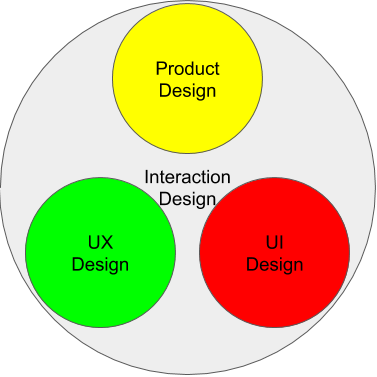
\includegraphics[width=0.8\textwidth]{../immagini/interactiondesign2.png}
	\caption{Il design dell'interazione è un un settore altamente interdisciplinare in cui si vanno a compenetrare diverse discipline.}
\end{figure}

Prima di entrare nel dettaglio è importante sottolineare che nessuna di queste discipline o settori della progettazione è rigidamente definite e spesso le tre si intrecciano e vengono quindi eseguite da team multi disciplinari. Inoltre, specialmente in piccole aziende e piccoli team di sviluppo non si riesce a separare queste attività di progettazione e quindi è estremamente importante che l'informatico moderno conosca i rudimenti di base necessari per poter contribuire ad un team in cui vengono portate avanti anche questa tipologia di attività.


\subsection{Product Design}
Il \textbf{design di prodotto} è un processo strategico di risoluzione dei problemi che guida l'innovazione e porta a una migliore qualità della vita attraverso prodotti, sistemi, servizi ed esperienze innovative \textit{(definizione ufficiale di disegno industriale, coniata nel 2015 dalla World Design Organization (ex ICSID). Spesso design di prodotto e design industriale sono utilizzati in modo intercambiabile}. 

Nel design di prodotto si progettano quindi beni e servizi il cui obbiettivo principale è quello di essere utilizzati da quanti più utenti possibili migliorandone la vita. Il designer di prodotto è quindi colui che inventa un nuovo modo o un nuovo oggetto per fare cose che fino a ieri non si potevano fare o si facevano in maniera più complicata.

Il design di prodotto è quindi il punto di partenza dei processi di innovazione e rappresenta quindi il punto di partenza del percorso di design dell'interazione che stiamo esplorando.

L'inventore (designer) del prodotto si focalizza su un problema da risolvere e inventa un prodotto che grazie alle sue caratteristiche tecniche permette di risolvere il problema.

Descriviamo un prodotto noto come se stessimo provando a formalizzare un processo di product design atto a reinventare un processo noto e consolidato, ascoltare musica. 

\begin{flushleft}
\textbf{Nome prodotto:} Spotify;\\
\textbf{Problema a cui assolve:} Ascoltare musica senza possederla;\\
\textbf{Tipologia di prodotto:} Servizio basato su Internet;\\
\textbf{Funzionalità principale:} Consentire l'ascolto di qualunque brano, su qualsiasi piattaforma senza richiedere l'acquisto di un supporto fisico e dei diritti d'autore;\\
\textbf{Soluzioni esistenti:} Noleggio/prestito CD e altri supporti fisici, download di musica pirata;
\textbf{Soluzione:} Servizio di streaming basato su business model "freemium" che di fatto rappresenta un jukebox con brani pressoché illimitati;
\textbf{Requisiti per l'utilizzo:} PC o smartphone o tablet, Connessione internet. 
\end{flushleft}

Estremizzando un po' i concetti potremmo dire che il product designer di Spotify ha terminato il suo lavoro. Quello sopra descritto è il frutto del processo di design di prodotto che ha portato alla nascita di un servizio rivoluzionario come Spotify. Non c'è tanto altro da aggiungere per descrivere il concetto che sta alla base del prodotto e quindi l'innovazione che esso introduce.

\begin{figure}[!h]
	\centering
	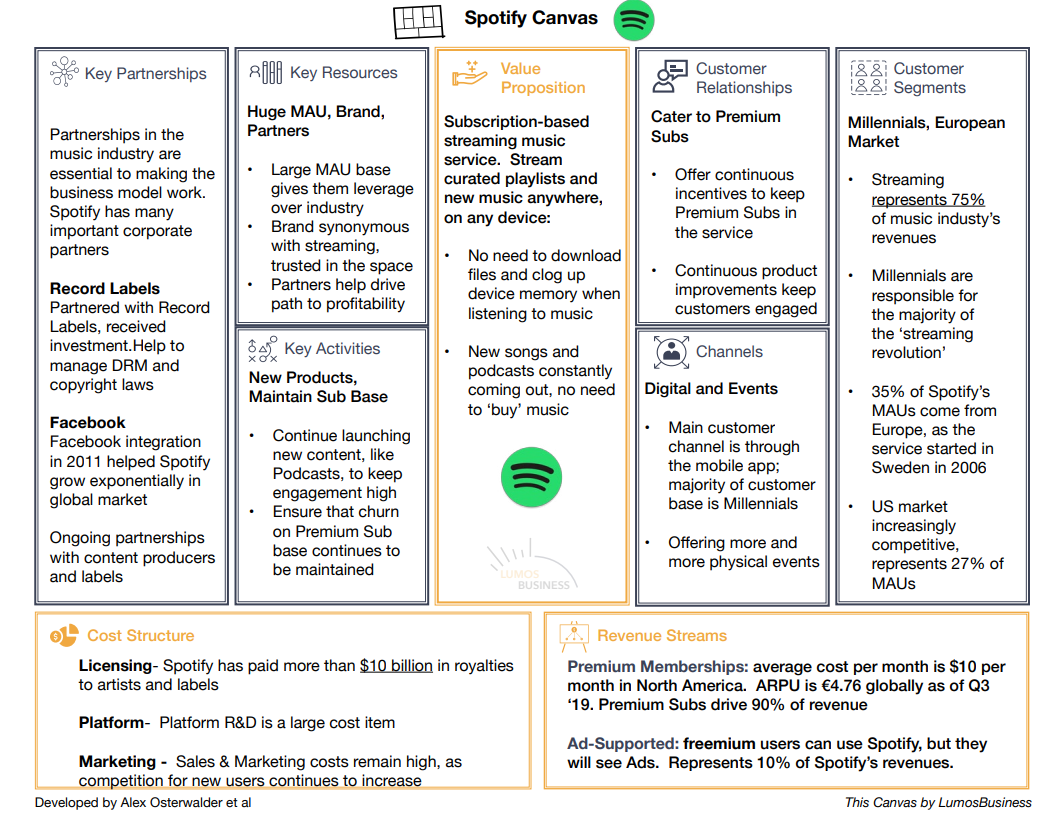
\includegraphics[width=\textwidth]{../immagini/spotifycanvas.png}
	\caption{Business model canvas di Spotify. Fonte http://lumosbusiness.com/business-model-canvas-spotify/}
\end{figure}

E' chiaro però che questo nuovo prodotto potrebbe essere realizzato in tanti modi e che sarà proprio il modo in cui viene costruito a decretarne il successo o il fallimento del prodotto. Questo perchè non basta un'idea per fare un prodotto di successo, ci vuole un lungo e complicato processo di progettazione che vada oltre l'idea e metta al centro l'utente, i suo bisogni e le sue aspettative.

\subsection{User Experience Design}
Il \textbf{design dell'esperienza utente} è il processo volto ad aumentare la soddisfazione e la fedeltà del cliente migliorando l'usabilità, la facilità d'uso e il piacere fornito nell'interazione tra il cliente e il prodotto. La progettazione dell'esperienza utente comprende la tradizionale progettazione dell'interazione uomo-macchina e la estende integrandola con tutti gli aspetti di business, marketing e sviluppo prodotto necessari per garantire il successo del prodotto e/o servizio.

%L'esperienza utente è qualsiasi aspetto di un'interazione della persona con un dato sistema informatico e interattivo. La progettazione dell'esperienza studia il prodotto nel suo insieme trattando aspetti legati all'interfaccia, alla grafica, alla progettazione industriale e all'interazione fisica e manuale.

Ogni prodotto durante l'utilizzo da parte di un utente porta a far vivere un esperienza e di conseguenza si dice abbia una sua ``user experience''. Ovviamente, la user experience non è una proprietà del prodotto in se ma piuttosto una relazione che intercorre fra il prodotto ed uno specifico utente. Il tema delle relazioni e della relatività delle esperienze verrà meglio affrontato nei capitoli successivi. 

%Per ora limitiamoci a sottolineare che non è possibile progettare l'esperienza utente ma si progetta \textbf{per} l'esperienza utente.

Lo \textbf{UX Designer} ha quindi l'obbiettivo di far vivere all'utente del suo prodotto la miglior esperienza possibile, evitando quindi che l'oggetto induca nell'utente sensazioni di frustrazione e delusione.
Spesso si tende a dire che si ``progetta l'esperienza utente''. In realtà è impossibile progettare l'esperienza utente perchè ogni utente è diverso dall'altro ed è quindi illusorio pensare che chiunque durante l'utilizzo del prodotto si comporti alla stessa maniera e in particolare si comporti esattamente come il progettista ha ipotizzato.
E' quindi corretto dire che si ``progetta \textbf{per} l'esperienza utente''.

Come vedremo nei capitoli successivi, lo studio e la progettazione dell'esperienza utente partono sempre dalla analisi e comprensione delle esigenze dell'utente e non dalle specifiche funzionali di prodotto. 

\subsection{User Interaction Design}
Il Design dell'interazione ha come focus il modo in cui le persone interagiscono con la tecnologia, lo scopo è migliorare la loro comprensione di ciò che si può fare, ciò che succede e ciò che è appena successo, basandosi su principi psicologici, tecnici ed estetici.

Dallo studio della UX si crea quindi uno schema di interazione che poi viene passato allo \textbf{UI Designer} che ha il compito di progettare l'interfaccia utente al fine di abilitare l'esperienza progettata.
%un abbozzo dell'interfaccia. Non si crea subito il \textit{wireframe} finale, bensì si parte da un'analisi dei casi di studio. Esistono più tipi di casi di studio ed ognuno è specifico per delle personas, infatti, personas differenti hanno capacità differenti.

Lo UI designer non costruisce quindi l'interfaccia utente, nei team numerosi questa figura è spesso un progettista grafico e non un informatico. L'obbiettivo dello UI designer è quello di progettare l'aspetto estetico e la struttura dell'interfaccia così che questa durante l'utilizzo induca l'utente nel seguire l'esperienza che è stata per lui progettata.
Lo UI designer produce quindi un wireframe, una bozza grafica, dell'interfaccia e una serie di linee guida che poi veranno seguite dagli sviluppatori (UI developer o Front-end developer) per implementare la reale interfaccia del prodotto o servizio

\begin{figure}[!h]
	\centering
	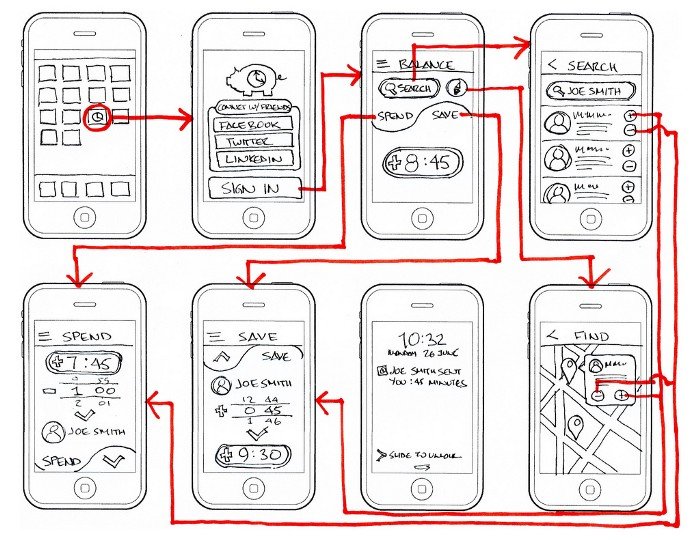
\includegraphics[width=\textwidth]{../immagini/uidesign.jpeg}
	\caption{Esempio di progetto di UI per una App mobile. Il wireframe riporta le linee guida per la struttura dell'interfaccia e il flusso utente (implementato a partire dal lavoro di UX Design). Fonte: https://blog.prototypr.io/why-you-shouldnt-skip-your-wireframing-1f7a70d5c125}
\end{figure}

%o differente dal front-end developing: la materia progetta le guidelines che istruiscono il developer su come creare al meglio una UI.

%Non è sbagliato considerare lo UI Design come \textbf{sotto area} dello UX Desing.

Il processo di Product Design è quindi un percorso strutturato che include varie figure e discipline. In grandi team questi step sono eseguiti tipicamente da diverse persone e team ma spesso nella media e piccola impresa o startup questo percorso deve poter essere seguito in autonomia da una o al massimo due figure.

L'interfaccia vera e propria viene implementata quindi solo alla fine del percorso di progettazione da figure con profilo tecnico informatico (Front End Developer o UI Developer). Queste figure devono quindi essere in grado di comprendere le richieste provenienti dagli step di progettazione precedenti e quindi devono possedere i rudimenti base dell'Interaction Design e delle relative sotto discipline.

\begin{figure}[!h]
	\centering
	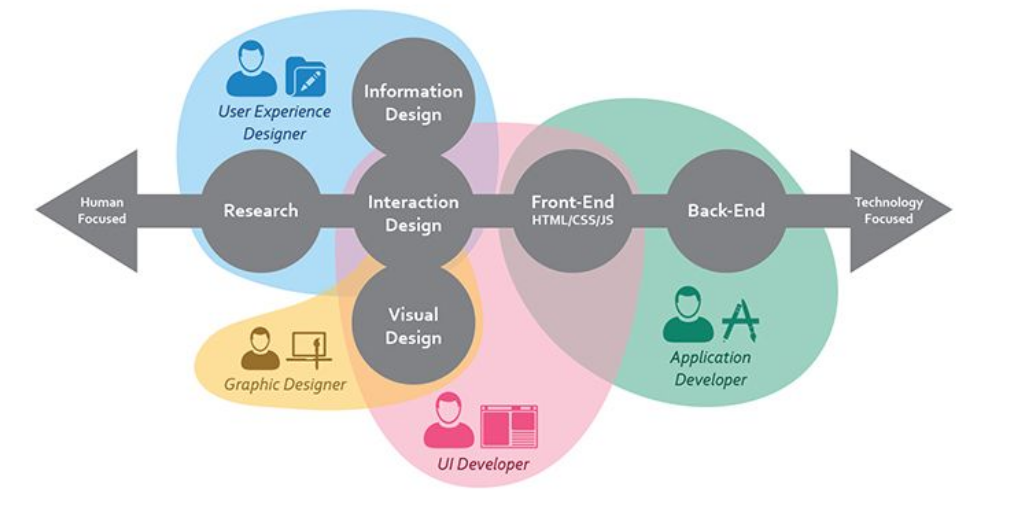
\includegraphics[width=\textwidth]{../immagini/UX_and_UI.png}
	\caption{Flusso di lavoro e ruoli necessari per lo sviluppo di un prodotto. fonte: https://www.crayondata.com/blog/the-difference-between-ui-and-ux/
}
\end{figure}

 %Progettare l'Interazione fra Uomo e Macchina
\chapter{Human Centered Design}

\textit{I progettisti devono produrre cose che soddisfino i bisogni della gente, in termini di funzioni, facilità d’uso e gratificazione emotiva. In altre parole, il design (di prodotto) deve essere pensato come un’esperienza totale (per l'utente).} 

[Donald Norman — La caffettiera del masochista]

Le persone sono sempre più frustate dalla complessità degli oggetti quotidiani. Dalla complessità sempre maggiore del cruscotto dell'auto, dalla lavatrice piena di incomprensibili funzioni e pulsanti, dalla crescente automazione della casa, e dalla continua proliferazione di funzioni che i progettisti aggiungono con orgoglio ad ogni nuova versione dei loro prodotti.

La vita della maggior parte degli utenti è ormai diventata una battaglia quotidiana per la sopravvivenza alla invadente e iper-funzionale tecnologia. %tutti i giorni sembra a volte una battaglia infinita contro la confusione, gli errori continui, la frustrazione e un ciclo interminabile di aggiornamenti e manutenzioni degli apparecchi.

Questo problema origina direttamente dalla modalità con la quale vengono oggigiorno progettati gli oggetti quotidiani ed in particolare quelli tecnologici. Le macchine (computer) hanno una modalità di funzionamento logica, dovuta all'algoritmo che il progettista ha sviluppato come anima della macchina. Noi umani invece siamo tutt'altro che logici e razionali, siamo intuitivi, flessibili, versatili e curiosi. È chiaro quindi che nell'interazione uomo-macchina si va a creare una relazione fra specie diverse che hanno modalità di pensiero e di funzionamento opposte.

Gli ingegneri e gli informatici, orgogliosi dei loro progressi tecnologici, hanno preteso da sempre che gli umani si adattassero alle loro macchine. Le macchine sono viste come un elemento di orgoglio che rappresenta il progresso e chi non è in grado di capirle è retrogrado, vecchio e a volte anche un po' stupido.

Questo approccio tecno-centrico dei progettisti ha in realtà leso lo sviluppo stesso della tecnologia dal momento che ne ha rallentato la sua diffusione e accettazione.
La maggior parte degli utenti oggi è frustrata dall'utilizzo di incomprensibili oggetti tecnologici di cui non capisce il principio di funzionamento e dove tipicamente si limita ad utilizzare il 10\% delle funzionalità disponibili.

Le macchine hanno delle loro regole di funzionamento che sono spesso note solo ai progettisti. Quando non si seguono queste regole le cose non vanno come previsto e l'utente si sente stupido ed incapace. La macchina è perfetta, non può sbagliare, quindi se le cose sono andate male è sicuramente colpa dell'umano. 
È vero ma non è l'umano utente ad aver sbagliato, la colpa è del progettista!

Nel design antropocentrico si inverte il paradigma di progettazione mettendo l'utente al centro del processo. Le funzionalità del prodotto vengono dopo. Prima ci sono i bisogni dell'utente!

Questo processo, apparentemente ovvio e banale, risulta in realtà estremamente difficile da applicare per gli informatici. I tecnici infatti amano le funzioni e funzionalità, amano le peculiarità tecniche dei sistemi e sono spesso spinti a sviluppare nuove soluzioni non tanto per risolvere problema ma piuttosto per soddisfazione personale di aver implementato qualcosa che prima non esisteva.

La blockchain è sicuramente un esempio di questo fenomeno. Creata per diletto da degli appassionati di crittografia, ha dato vita alla prima cryptomoneta della storia. Dopo il boom di Bitcoin e delle altre cryptomonete è scoppiata la bolla blockchain dove tutti nel mondo IT hanno iniziato a dichiarare che grazie alla blockchain si sarebbe potuto innovare in maniera radicale tantissimi settori. Ad oggi in realtà dopo aver lanciato numerosi bandi di concorso in tutto il mondo, aver aperto fondi di investimento dedicati alle startup che utilizzano tecnologia blockchain non si è ancora trovata una applicazione di successo, oltre alle cryptomonete, che senza blockchain non sarebbe realizzabile.

Per dirla in altre parole, nessun utente ci ha chiesto di sviluppare la blockchain in quanto tale, c'era bisogno di scambiarsi denaro in maniera alternativa e quindi sono nate le cryptomonete. Ora la corsa a cercare di applicare la blockchain ad altri settori non sta funzionando perché non esiste il problema da risolvere! Stiamo cercando un problema per una tecnologia ma bisognerebbe cercare tecnologie che risolvono problemi!

La morale di questo ragionamento è: se vogliamo progettare tecnologia per le persone dobbiamo capire sia la tecnologia che le persone. Dobbiamo pensare a risolvere i problemi delle persone, non a crearne di nuovi perché dobbiamo bulimicamente sviluppare nuova tecnologia.


Questo vuol dire passare da un approccio tecno-centrico ad uno antropocentrico. Lo human centered desing o HCD, è una \textbf{metodologia di progettazione che parte dai bisogni, dalle capacità e dai comportamenti umani, adattando la progettazione a quei bisogni, quelle capacità e quei comportamenti}. Lo HCD è un approccio di design specificamente orientato allo sviluppo di sistemi interattivi, con l'obiettivo quindi di produrre sistemi utili, altamente usabili e che si \textbf{focalizzino sull'utente}.

Il design antropocentrico è orientato all'efficienza ed all'efficacia e punta quindi ad aumentare la soddisfazione dell'utente durante l'utilizzo del prodotto e ad evitare il più possibile gli effetti negativi e quindi indurre frustrazione.\\

\textbf{Prima l'utente, poi le features!} \\

Lo HCD mette i bisogni, comportamenti e capacità umane prima di tutto e progetta in funzione di esse. Per questo motivo il processo HCD parte dall'osservazione dell'utente, dei suoi comportamenti e quindi dallo studio dei suoi bisogni per poi arrivare solo dopo all'identificazione della tecnologia necessaria.

Il problema principale delle UI è la comunicazione fra uomo e macchina. L'interazione uomo-macchina è una forma di dialogo inter-specie; due soggetti aventi culture, corpi e lingue diverse si trovano a dover interagire per risolvere insieme un problema che uno dei due (l'umano) ha. 
%, in particolare la comunicazione dalla macchina verso l'uomo, \textbf{una buona interfaccia \textit{sa} comunicare con l'utente}.

\begin{figure}[!h]
	\centering
	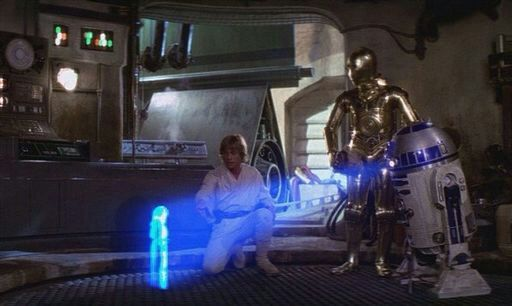
\includegraphics[width=\textwidth]{immagini/starwars.jpg}
	\caption{La tecnologia è percepita come utile quando è possibile comunicarci per risolvere insieme problemi.}
\end{figure}

Progettare interfacce che funzionano fintanto che le cose vanno bene è relativamente facile, ma \textbf{la comunicazione è ancora più importante quando le cose non vanno bene}. È qui che i progettisti devono concentrare l'attenzione, sui casi in cui le cose vanno storte, non su quelli in cui le cose funzionano secondo i piani. 


Dobbiamo smettere di progettare per le persone come vorremmo che fossero e iniziare a progettare per come realmente sono!

Questo approccio è valido sempre, non solo nello sviluppo tecnologico. Un buon avvocato scrive un contratto in previsione di cosa potrebbe andare male nella relazione fra le parti. Se le cose dovessero andare bene sicuramente le parti non avranno bisogno del contratto e questo verrà dimenticato in un cassetto. Il contratto diventa utile quando qualcosa va storto e se ben fatto rende la gestione del problema molto più semplice, veloce e quindi potenzialmente indolore. 

È quindi bene focalizzare sempre l'attenzione su ciò che potrebbe andare storto durante l'interazione così da progettare accuratamente la comunicazione e guidare quindi l'utente verso la risoluzione del problema così da ridurre la frustrazione e quindi la negatività verso il prodotto. 

Non bisogna aver paura che l'utente abbia problemi o che il nostro software abbia degli errori o bug, è inevitabile che questo accada. È importante progettare perché l'utente venga guidato nella risoluzione e gestione dell'errore senza provare frustrazione. Avremo così un utente soddisfatto. 

L'esperienza di utilizzo produce emozioni negli utenti, più emozioni positive (successi) l'utente avrà e migliore sarà la percezione che avrà del nostro prodotto. È importante sottolineare inoltre che la memoria ha la capacità di far provare sensazioni più profonde rispetto al presente. Un utente che di fronte ad un problema riesce a risolverlo perché ben guidato dalla tecnologia avrà memoria di un suo successo. Questo tipo di sensazioni sono molto forti e se associate al prodotto fanno si che l'utente sviluppi empatia per il prodotto e che quindi lo apprezzi e ne senta il bisogno.

L'obiettivo dello HCD deve essere quindi quello di \textbf{creare nell'utente empatia verso il sistema}.

%\textbf{Evitare quindi la frustrazione e aiutare nella risoluzione quando insorge un problema sono i concetti chiave dello HCD.}
%Lo HCD è una filosofia di design che parte dalla \textbf{comprensione delle persone e dei bisogni che esse intendono soddisfare}. Questa comprensione deriva dall'osservazione e dallo studio delle persone che spesso sono inconsapevoli dei loro veri bisogni e magari anche delle difficoltà che incontreranno.

L'HCD è una forma di pensiero ed è quindi compatibile con le varie discipline del design di prodotto che abbiamo precedentemente introdotto (vedere figura \ref{hcd}). 
Si può infatti applicare il pensiero HCD sia al design industriale che alla progettazione dell'interazione o dell'esperienza utente: lo \textbf{HCD non è un'area o un metodo, è una forma di pensiero.}

\begin{table}[!h]
	\center
	\begin{tabular}{ll}
		\multicolumn{2}{c}{\textbf{Il ruolo dello HCD nel design}} \\ \hline
		\multicolumn{1}{c|}{Experience design} & Area di focus     \\ \hline
		\multicolumn{1}{c|}{Industrial design} & Area di focus     \\ \hline
		\multicolumn{1}{c|}{Interaction design} & Area di focus    \\ \hline
		\multicolumn{1}{c|}{Human Centered Design} & \begin{tabular}[c]{@{}l@{}}Il processo che assicura\\ che la progettazione in-\\ contri i bisogni e le ca-\\ pacità degli utenti che \\ useranno il sistema\end{tabular}
	\end{tabular}
\end{table}

%\begin{figure}[!h]
%	\centering
%	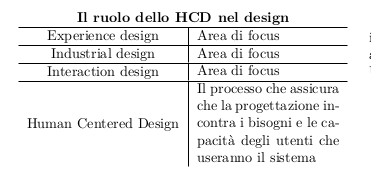
\includegraphics[width=0.7\textwidth]{immagini/HCD}
%	
%	\label{hcd}
%\end{figure}

A sottolineare quanto l'HCD sia ritenuto oggigiorno fondamentale per la progettazione di sistemi destinati all'utilizzo umano, è importante ricordare che il design antropocentrico è ormai parte della norma ISO EU. \\

\textbf{ISO 9241-210:2019 Ergonomics of human-system interaction\\ Part 210: Human-centred design for interactive systems}\\

\textit{This document provides requirements and recommendations for human-centred design principles and activities throughout the life cycle of computer-based interactive systems. It is intended to be used by those managing design processes, and is concerned with ways in which both hardware and software components of interactive systems can enhance human-system interaction.}

\textit{Computer-based interactive systems vary in scale and complexity. Examples include off-the-shelf (shrink-wrap) software products, custom office systems, process control systems, automated banking systems, Web sites and applications, and consumer products such as vending machines, mobile phones and digital television. Throughout this document, such systems are generally referred to as products, systems or services although, for simplicity, sometimes only one term is used. This document provides an overview of human-centred design activities. It does not provide detailed coverage of the methods and techniques required for human-centred design, nor does it address health or safety aspects in detail. Although it addresses the planning and management of human-centred design, it does not address all aspects of project management. }

\textit{The information in this document is intended for use by those responsible for planning and managing projects that design and develop interactive systems. It therefore addresses technical human factors and ergonomics issues only to the extent necessary to allow such individuals to understand their relevance and importance in the design process as a whole. It also provides a framework for human factors and usability professionals involved in human-centred design.}

\textit{Detailed human factors/ergonomics, usability and accessibility issues are dealt with more fully in a number of standards including other parts of ISO 9241 (see Annex A) and ISO 6385, which sets out the broad principles of ergonomics.}

\url{https://www.iso.org/standard/77520.html}\\

Un buon processo HCD parte, come abbiamo detto, dall'osservazione dell'utente e dei suoi bisogni. Tuttavia, tale osservazione non è sempre possibile o facile da attuare. Nei successivi capitoli analizzeremo varie tecniche di prototipazione rapida e metodi di lavoro finalizzati all'estrazione veloce di bisogni utente e all'esecuzione rapida e a basso costo di test. 

Possiamo schematizzare un processo di HCD come un flusso continuo ed iterativo che attraversa le seguenti fasi: 
\begin{itemize}
    \item \textbf{Specificare il contesto d'uso:} identificare gli utenti che utilizzeranno il prodotto, per cosa lo utilizzeranno e sotto quale condizioni e vincoli;
    \item \textbf{Specificare i Requirements:} Identificare i business requirement e gli obiettivi utente che devono essere raggiunti grazie all'utilizzo del software;
    \item \textbf{Progettare la soluzione:} questa fase può essere a sua volta spacchettata in sotto fasi iterative. Si passa tipicamente dadelle bozze a dei prototipi e poi alla soluzione;
    \item \textbf{Testare e valutare:} è fondamentale testare e quindi valutare il sistema così da poter iniziare il ciclo sulla base dei risultati dei test e quindi procedere ad uno sviluppo e miglioramento incrementale.
\end{itemize}

\begin{figure}[!h]
	\centering
	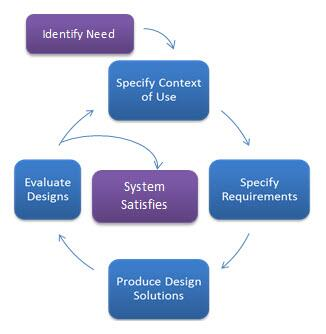
\includegraphics[width=0.8\textwidth]{immagini/HCD-chart}
	\caption{Flusso di lavoro tipico di un processo di design antropocentrico. Fonte: https://www.usability.gov/what-and-why/user-centered-design.html}
	\label{hcd-chart}
\end{figure}

Per ora, al fine di inquadrare meglio la filosofia HCD nel contesto dello sviluppo software vi basti pensare che le versioni alfa e beta dei nostri software possono diventare potenti strumenti di analisi degli utenti. Le versioni di test non servono quindi solamente a fare debugging del codice e delle funzioni, ma servono anche e sopratutto a capire che cosa fanno e come si comportano gli utenti durante l'utilizzo del nostro software.

Nello sviluppo software diventa quindi indispensabile abilitare dei sistemi di tracking dell'utente finalizzati alla produzione di statistiche di utilizzo. Avere zero errori (segnalazioni di bug) su una funzionalità che nessuno usa non vuol dire che questa sia perfetta ma soprattutto vuol dire che non aveva senso implementarla e quindi non ha senso mantenerla. Viceversa, avere alti utilizzi di una funzionale che era stata pensata come opzionale o accessoria ci deve indurre a pensare che invece gli utenti hanno trovato quel processo più utile e soddisfacente rispetto a quello che in fase di progettazione il designer aveva pensato come ``principale'' e quindi fondamentale.


\section{Usabilità}
%Ottenere \textbf{le specifiche dello HCD} è quindi una delle parti più difficili del design stesso, al punto che il principio è quello \textbf{di evitare di specificare il più al lungo possibile} e procedere con ripetute approssimazioni: si esegue una specifica ad alto livello, se ne implementa una parte, si testa sull'utente finale e tramite il suo feedback, si modifica la parte implementata e la si testa di nuovo. Fatto ciò si passa, magari momentaneamente, ad implementare un'altra parte.

Secondo la norma ISO, per usabilità si intende il \textit{``grado in cui un prodotto può essere usato da particolari utenti per raggiungere certi obiettivi con efficacia, efficienza e soddisfazione in uno specifico contesto d’uso''.} 

Sul sito dell'Agenzia per l'Italia digitale (\url{https://www.agid.gov.it/it/design-servizi/usabilita}) si legge: \\

\textit{L'usabilità è un carattere imprescindibile nella realizzazione di un portale web, perché permette di creare un ambiente familiare per l'utente, determinando numerosi vantaggi:}

\begin{itemize}
    \item \textit{consente di trovare e comprendere informazioni in modo più semplice e intuitivo;}
    \item \textit{facilita la memorizzazione e l'apprendimento dei contenuti presenti;}
    \item \textit{permette una riduzione dei costi e degli errori di sviluppo;}
    \item \textit{rende l'utente più autonomo e sicuro nel rapporto con lo strumento.}
\end{itemize}

\textit{L'usabilità mira a ridurre la distanza tra il cittadino e le amministrazioni, permettendo agli utenti di trovare le informazioni necessarie, comprenderne i contenuti ed eliminare le difficoltà di utilizzo di un determinato sito istituzionale.}\\

Si nota subito che il tema dell'usabilità è spesso associato esclusivamente al mondo del web e dello sviluppo di siti internet. L'usabilità è quindi intesa come la disciplina che regola la costruzione del sito o applicazione sulla base delle esigenze dell’utente, cercando di semplificare la sua esperienza di navigazione.

Questa è ovviamente un'errata semplificazione dovuta a come in diversi settori dell'informatica si siano adottate terminologie diverse per esprimere concetti simili se non equivalenti. Nel mondo del design di oggetti interattivi per esempio, l'usabilità è talmente importante che viene quasi data per assodata e il suo studio è spacchettato in diverse sotto attività e quindi risulta più raro trovare delle attività dedicate allo studio dell'usabilità in quanto tale.

Il tema dell'usabilità e del design antropocentrico si applicano (si dovrebbero applicare) quindi, a tutto il mondo dello sviluppo di prodotto. Ogni oggetto, artefatto, software o sistema destinato all'utilizzo da parte di utenti (umani) necessita che se ne studi la relativa usabilità e che intorno a questa si progetti il sistema stesso (HCD).

Una risorsa molto interessante e ben fatta sul tema dell'usabilità di servizi destinati ai cittadini è \url{https://designers.italia.it/}. Sul portale, nato nel 2017, sono presenti numerose linee guida e forum di conversazione relativi allo sviluppo di software per la Pubblica Amministrazione. 

\begin{figure}[!h]
	\centering
	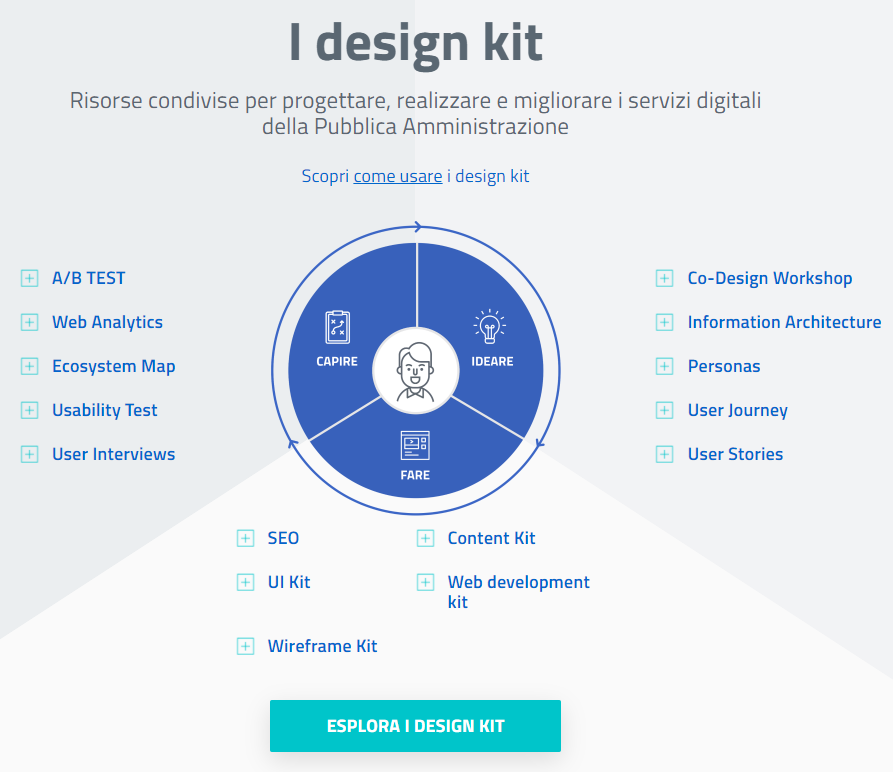
\includegraphics[width=0.8\textwidth]{immagini/designeritalia}
	\caption{https://designers.italia.it/ Mette a disposizione varie linee guida e strumenti per la progettazione antropocentrica di servizi dedicati alla pubblica amministrazione.}
	\label{designersitalia}
\end{figure}
 %Human Centered Design
\chapter{Progettazione delle interfacce}
Esistono solo due tipi di design, riuscito e fallito; buono e cattivo (D. Norman).

Il problema è che il buon design non è universale. Un progetto, prodotto o sistema apprezzato da tutti non esiste perché l'esperienza di interazione è soggettiva e quindi dipende più dalla persona che non dall'artefatto e di conseguenza è statisticamente impossibile progettare qualcosa che sia apprezzato da chiunque.

Nel corso vedremo come classificare gli utenti in gruppi e categorie così da poter identificare degli archetipi di persona per i quali andare a progettare l'interazione nella speranza di ottenere dei prodotti che almeno da alcune persone selezionate vengano apprezzati.

Questo perché è bene ricordare che non è possibile progettare l'esperienza di un utente ma si può lavorare per progettare un prodotto che guidi l'utente verso una particolare esperienza da noi identificata come ottimale.

Ci sono due proprietà che sono fondamentali per qualsiasi progetto destinato ad essere utilizzato da persone: Discoverability (rilevabilità) e Understanding (comprensibilità)

\textbf{Discoverability:} è la capacità di un sistema di veicolare e comunicare i propri possibili usi all'utente. Un sistema che a prima vista fa capire all'utente a cosa serve e che cosa ci si può fare ha una buona discoverability. Per avere una buona discoverability si usa tipicamente la \textbf{visibilità}. Se le funzioni dell'oggetto sono visivamente eclatanti è probabile che l'oggetto abbia una buona discoverability.

Un rubinetto con i pomelli ha una discoverability migliore di un rubinetto automatico perché le sue funzioni sono più facilmente identificabili grazie a una maggiore visibilità dei controlli.


\begin{figure}[!h]
	\centering
	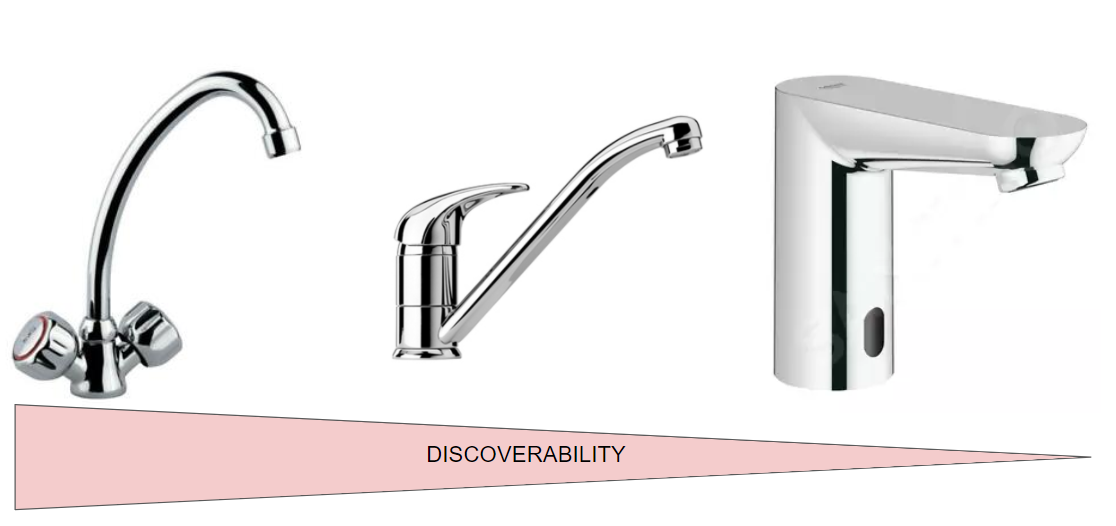
\includegraphics[width=\textwidth]{immagini/discoverability.png}
	\caption{Discoverability and visibility.}
\end{figure}


\textbf{Understanding}: è invece la capacità del prodotto di farsi usare correttamente dall'utente. Se la discoverability è la misura di quanto bene si capisce \textbf{cosa} si può fare con il prodotto, l'understanding invece è la proprietà associata a quanto bene un prodotto dice \textbf{come} si usano le funzioni disponibili.

Per capire come si usa un prodotto non basta infatti aver identificato quali sono i controlli, è necessario dare con facilità risposta alle seguenti domande:

\begin{itemize}
    \item Come si usa il prodotto?
    \item Che funzione ha ciascun controllo?
    \item Come si combinano i controlli?
    \item...
\end{itemize}




\begin{figure}[!h]
	\centering
	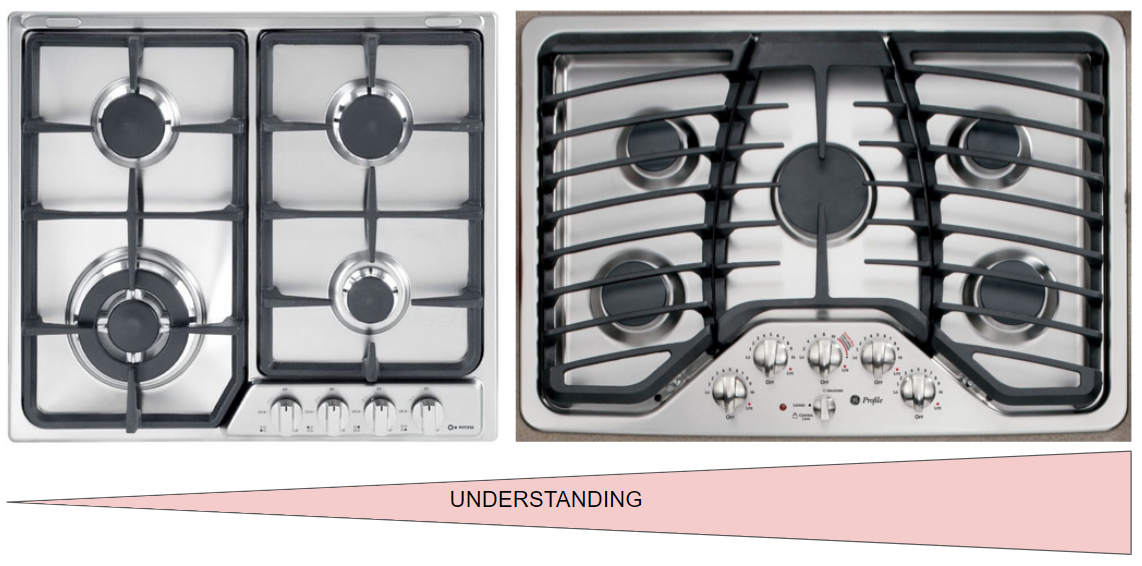
\includegraphics[width=\textwidth]{immagini/understanding.png}
	\caption{Understanding.}
\end{figure}


\section{Design of Useful Things}
\begin{flushleft}
	\textit{Quando le cose vanno bene, si dimenticano subito, quando vanno male non si dimenticano mai!}
\end{flushleft}

Questo fenomeno è noto a tutti, si tende a ricordare più facilmente le disavventure e i problemi che le belle esperienze, che spesso vengono percepite come ovvie e scontate. Questo accade perché ormai viviamo in una società in cui \textbf{le cose devono andare bene} per definizione. Quando qualcosa invece va storto, scattano tutta una serie di reazioni che portano la persona a provare sensazioni e emozioni spiacevoli, tipicamente frustrazione. 

Questo è un processo neurologico del tutto naturale che consente agli uomini di apprendere velocemente dalla propria esperienza andando ad etichettare le esperienze spiacevoli come più importanti rispetto a quelle positive. Dal punto di vista evolutivo, sbagliare vuol dire rischiare la vita mentre fare bene è solo l'ovvio cammino per la sopravvivenza.

Il design deve quindi preoccuparsi di come funzionano le cose, come vengono controllate e della natura delle interazioni che questi oggetti e sistemi abilitano con gli utenti. Gli oggetti, i software e i sistemi ben progettati danno vita ad esperienze d'uso piacevoli e rilassanti, quando un oggetto o un software sono mal progettati l'utente vive invece un'esperienza spiacevole caratterizzata da emozioni negative e dal desiderio di evitare in futuro di doversi imbattere nuovamente in un'esperienza simile.

Questo vuol dire che una cattiva esperienza utente induce l'utilizzatore non solo ad abbandonare l'utilizzo di un prodotto ma soprattutto porta la persona ad etichettare il prodotto e l'azienda produttrice come da evitare. 

Le \textbf{macchine} sono concepite, progettate e costruite da esseri umani ma sono ben diverse dai loro creatori. Le macchine sono sistemi logici, deterministici, prevedibili e con comportamenti basati su algoritmi fissi. L'uomo è invece aleatorio, versatile, variabile, volubile, e intuitivo. \textbf{Uno l'opposto dell'altro!}
Inoltre, le macchine non hanno esperienza (nell'accezione in cui la intendiamo tipicamente in neuroscienze). Per una macchina ogni azione, procedura e sequenza è nuova, si ricomincia sempre da zero. Non importa se l'utente ha già fatto quella procedura decine di volte, anche questa volta la macchina pretenderà che questa venga eseguita alla perfezione e seguendo tutti i passi richiesti.

Inoltre, le macchine al nostro confronto, sono \textbf{assai limitate}. Non possono fare qualsiasi cosa in maniera mediocre come noi ma sono concepite per fare poche cose (spesso solo una) in maniera eccellente. Anche in questo caso hanno un comportamento opposto rispetto a quello umano. Gli uomini sono in grado di fare tutto in maniera mediocre e qualche cosa in maniera eccellente e possono inoltre, con l'esperienza, cambiare le attività su cui eccellono. Le macchine nascono in un modo e muoiono invariate.

Le macchine seguono, di solito, \textbf{regole di comportamento rigide}, piuttosto complicate. Se si sbaglia nel seguirle, anche di poco, il sistema fallisce. La macchina esegue infatti quello che gli è stato richiesto, anche se questo è insensato e illogico. 

Questa analisi ci porta a concludere che \textit{le macchine obbligano le persone a smettere di comportarsi da umani inducendole a comportarsi da macchine.}

La tipica esperienza d'uso di un software è quella di un umano che impara le procedure imposte dal software, capisce come questo funziona ed è stato progettato e inizia così a ragionare come lui. L'umano asseconda la macchina per poter ottenere un risultato e procedere nell'esecuzione dell'attività senza intoppi.

\begin{flushleft}
	\textit{We have to humanize machines instead of dehumanizing humans} (David Hanson, Padre del robot Sophia della Hanson Robotics.)
\end{flushleft}

Questo condizione di schiavitù umana è dovuta al fatto che spesso le regole di funzionamento della macchina sono note solo alla macchina stessa e ai suoi progettisti. 

Come detto, quando non si eseguono queste regole segrete e bizzarre, la macchina fa la \textbf{cosa sbagliata} e la colpa è tipicamente accollata all'utente incapace. Quando questo accade con oggetti comuni, di uso domestico o personale, il risultato è la frustrazione dell'utente e il fallimento del prodotto. Quando invece questo fenomeno accade in contesti industriali e commerciali, le conseguenze possono essere incidenti mortali e importanti conseguenze economiche.

È tempo di \textbf{ribaltare la prospettiva}. 

\begin{flushleft}
	\textbf{Quando le cose vanno male la colpa non è mai dell'utente ma è sempre della macchina e quindi del progettista.}
\end{flushleft}

Questa prospettiva, apparentemente estrema, è in realtà il punto di partenza fondamentale per la progettazione di prodotti, sistemi e servizi usabili e quindi di successo. 

Le ragioni della complessità dell'interazione uomo-macchina sono numerose. Spesso però, la maggior causa del ``cattivo design'' è dovuta alla formazione dei tecnici e dei progettisti. Per molti anni si è focalizzato tutto il bagaglio formativo dei tecnici su tematiche tecnologiche ignorando gli aspetti legati alla psicologia umana e alle dinamiche di mercato.

La maggior parte dei problemi di design deriva quindi dalla totale incomprensione dei principi del design necessari per portare alla realizzazione di un prodotto capace di abilitare una positiva esperienza di interazione uomo-macchina.

Gli ingegneri, gli informatici sono eccellenti sul piano tecnico ma spesso sono molto limitati nella comprensione delle persone e della socialità.
I tecnici pensano: \textit{``Siamo uomini anche noi, quindi siamo in grado di capire i nostri simili e di progettare per loro.''}

Sbagliato! I tecnici falliscono perché partono da un'assunzione profondamente sbagliata e cioè che la spiegazione logica del funzionamento di un sistema sia sufficiente per consentire a chiunque di utilizzarlo. Purtroppo, come già detto, la logica e le persone non vanno molto d'accordo!

\begin{flushleft}
\textit{``Basterebbe che leggessero le istruzioni e tutto andrebbe bene!''}
\end{flushleft}


Gli ingegneri sono formati per utilizzare quotidianamente il pensiero logico e computazionale, di conseguenza finiscono per credere che quello sia il modo comune di ragionare. 


È quindi fondamentale accettare che il comportamento umano è illogico e non può essere modificato (per fortuna). 
\begin{flushleft}
\textbf{Bisogna progettare per come le persone sono e non per come vorremmo che fossero!}
\\
\textit{``we were designing things for people, so we needed to  understand both technology and people. But that’s a difficult step for many engineers: machines are so logical, so orderly. \\
If we didn’t have people, everything would work so much better. \\
Yup, that’s how I used to think.'' (Donald Norman)}
\end{flushleft}

\section{L'incidente di Three Mile Island }
Da: \url{https://it.wikipedia.org/wiki/Incidente_di_Three_Mile_Island}\\

L'incidente di Three Mile Island fu una parziale fusione del nocciolo avvenuto nella centrale nucleare sull'omonima isola, nella Contea di Dauphin, in Pennsylvania, il 28 marzo del 1979. Fu il più grave incidente nucleare avvenuto negli Stati Uniti d'America, e ha portato al rilascio di piccole quantità di gas radioattivi e di iodio radioattivo nell'ambiente.


L'incidente avvenne esattamente alle ore 4:00 di mercoledì 28 marzo 1979, quando il reattore era ad un regime di potenza del $97\%$. L'incidente ebbe inizio nel circuito di refrigerazione secondario, con il blocco della portata di alimentazione ai generatori di vapore. Questo blocco portò, nel circuito primario di raffreddamento del nocciolo, ad un considerevole aumento della pressione del refrigerante, causando prima l'apertura di una valvola PORV di rilascio posta sul pressurizzatore e poi lo ``SCRAM'' (arresto di emergenza del reattore mediante l'inserimento delle barre di controllo). 

A questo punto la valvola di rilascio non si richiuse e \emph{gli operatori non si resero conto del problema, anche perché non vi era nella strumentazione l'indicazione della reale posizione della valvola. La strumentazione era infatti legata all'alimentazione del motore della valvola e non alla reale posizione della valvola.}

Fu così che il circuito di raffreddamento primario si vuotò parzialmente e il calore residuo del nocciolo del reattore non poté essere smaltito. A causa di ciò il nocciolo radioattivo subì gravi danni. \emph{Gli operatori non poterono diagnosticare correttamente cosa avveniva e reagire in maniera adeguata. La strumentazione carente della sala controllo e l'addestramento inadeguato risultarono essere le cause principali dell'incidente.}

Durante l'incidente si ebbe una pericolosa fusione parziale del nocciolo e di conseguenza vennero riportati alcuni gravissimi danni; l'unità 2 fu chiusa ed è ancora oggi sotto monitoraggio, in attesa delle future azioni di smantellamento.

%I dispositivi complessi a causa della loro scarsa visibilità e della loro complessità richiedono di essere accompagnati da manuali d'istruzioni, ma questo è accettabile \textbf{solo} se il dispositivo è davvero complesso e dovrebbe essere del tutto \textbf{superfluo} per le cose \textbf{semplici}.

 %Progettazione delle interfacce
\chapter{Principi Fondamentali dell'Interazione}
Un buon design produce un'esperienza piacevole! Ai tecnici non piace molto la parola \textit{esperienza} poiché la considerano troppo soggettiva e poco legata alla tecnologia ed al progresso. Ma se chiediamo ad un ingegnere di descrivere la sua automobile preferita descriverà modello e finiture, dettagli tenici e poi ci narrerà la sensazione che ha provato quando era alla guida: la potenza percepita dall'accelerazione, la maneggevolezza del cambio e dello sterzo, la sensazione di aderenza etc..

L'esperienza è cruciale nell'utilizzo di qualsiasi sistema tecnologico o no che sia. E' grazie all'esperienza che si crea \textbf{la tonalità del ricordo} che conserviamo e associamo agli oggetti con cui abbiamo interagito.

Quando la tecnologia si comporta in maniera inaspettata, gli utenti provano confusione, frustrazione e rabbia: tutte \textbf{emozioni negative}. L'utente che invece riesce a comprendere il funzionamento, e quindi ad utilizzare correttamente un prodotto, proverà una piacevole sensazione di controllo, sarà soddisfatto e persino orgoglio. Tutte queste sensazioni positive saranno associate al prodotto!

\textbf{Cognizione ed emozione sono profondamente legate}: se non si mette l'utente in uno stato mentale positivo e quindi propenso alla sperimentazione e all'interazione, inevitabilmente l'utente compierà più errori perchè avrà un basso interesse per l'oggetto e farà più fatica ad usare l'interfaccia. Più l'utente è arrabbiato e frustrato meno è predisposto ad interagire e quindi imparare come si usa il prodotto e quindi riutilizzarlo in futuro.

Come abbiamo detto nel capitolo precedente, la \textbf{visibilità} o \textbf{discoverability} di un prodotto è il grado di facilità con cui un utente \textbf{scopre cosa può fare, come funziona e che tipo di azioni sono possibili} con il prodotto. 

Tale visibilità si ottiene attraverso il processo di design dell'interazione ed è il risultato dell'applicazione di cinque concetti psicologici fondamentali: 

\begin{itemize}
    \item \textbf{affordance}
    \item \textbf{significanti}
    \item \textbf{mapping} 
    \item \textbf{feedback}
    \item \textbf{vincoli}
\end{itemize}

C'è poi un sesto principio che come vedremo non è legato a degli elementi specifici dell'interfaccia ma piuttosto al concetto generale su cui si va a basare il funzionamento del sistema, \textbf{il modello concettuale del sistema}. Il modello concettuale di un sistema è il cuore dell'interazione e su questo si fonda l'intera esperienza utente.

\section{Affordance}
Il termine affordance, letteralmente \textit{invito}, indica la relazione fra le proprietà di un oggetto o sistema e le proprietà del suo utilizzatore. 

Le affordance non sono quindi proprietà oggettive di un sistema o prodotto ma piuttosto relazioni prodotto-utente che se stabilite abilitano o disabilitano specifiche modalità di interazione fra le parti.

Una sedia appare fatta apposta per sostenere qualcosa quindi \textbf{invita} alla seduta. La maggior parte delle sedie è abbastanza leggera da poter essere sollevata e spostata da una persona possiamo quindi affermare che\\

\textit{una sedia presenta l'affordance per il "sedersi" e per "essere sollevata" da una persona adulta normodotata.}

La sedia non ha infatti la proprietà \textbf{universale} di consentire la seduta a chiunque. Un neonato non riesce a salire su una sedia e non riesce a stare seduto se non ha un sostegno laterale. La sedia non è quindi utilizzabile per sedersi da un neonato quindi per questo utente la sedia NON HA l'affordance del consentire la seduta.

Stessa cosa per la sollevabilità, un bambino di 3 anni può sedersi su una sedia ma non ha abbastanza forza per sollevarla. Quindi, anche in questo caso abbiamo un'affordance che non è disponibile con una categoria di utenti ma lo diventa con altre.

Un'affordance \textbf{non è una proprietà, è una relazione tra un oggetto e utente}, dipende quindi dalle proprietà sia dell'oggetto che dell'utente.

Oltre alle affordance esistono anche le \textbf{anti-affordance}. Un' anti-affordance è una relazione fra oggetto e utente che se stabilita va a negare, vietare alcune proprietà o modi di interazione disponibili fra utente e oggetto.
Un esempio di anti-affordance sono gli "spunzoni" usati come deterrenti per i volatili sui cornicioni, insegne etc. Questo sistema nega all'utente (piccione) di posarsi sul cornicione disabilitando di fatto la altrimenti presente affordance della stazionabilità, supporto, che altrimenti il piccione sarebbe in grado di abilitare e quindi usufruirne.

Le affordance e le anti-affordance per abilitare o disabilitare una particolare modalità di interazione fra oggetto ed utente \textbf{devono essere percepibili, "discoverable"}.

La percepibilità di un affordance non è certo un aspetto ovvio e che può essere dato per scontato. Il vetro, famoso per la sua trasparenza ha "afforda" per la trasmissibilità della luce ma ha un' anti-affordance per l'attraversabilità. Il vetro infatti non consente il passaggio di corpi solidi. Essendo trasparente, questa anti-affordance non è facilmente percepibile dall'utente e quindi l'utente può attuare interazioni non permesse dando origine a problemi di utilizzo (sbattere sulla porta a vetri).

Se uno di questi inviti o impedimenti all'uso non è percepibile c'è bisogno di aumentarne la visibilità e quindi la perceione da parte dell'utente al fine di rendere l'afforndance o anti-affordance percepita e quindi stabilire la corretta modalità di interazione fra utente e oggetto. Per dare visibilità ad un'affordance si usano i \textbf{significanti}.

Spesso nei testi di design si trovano affermazioni tipo: "\textit{E' stata messa un'affordance per...}". Le affordance non si mettono o si tolgono, le affordance sono modalità dell'interazione che nascono da relazioni fra proprietà dell'oggetto e proprietà dell'utente. Per abilitare delle affordance rendendole visibili e quindi palesi all'utente si inseriscono dei significanti che vanno solamente a aumentare la visibilità e compnresione di affordance già presenti.

\section{Significante}
I progettisti hanno dei problemi pratici: hanno bisogno di sapere come rendere comprensibili gli oggetti che creano. Lavorando sulla grafica degli schermi elettronici, dovevano trovare il modo di indicare quali parti potevano essere sfiorate, battute, fatte scivolare in sù, in giù o di lato, azioni che si potevano eseguire con le dita, con lo stilo o con il mouse.

Un significante è quindi \textbf{un modo per indicare dove effettuare un'azione}, data un'affordance che determina quali azioni sono possibili.

\begin{figure}[!h]
	\centering
	\includegraphics[scale = 0.7]{"../immagini/Affordance vs Signifier"}
\end{figure}
\begin{itemize}
	\item \textbf{Affordance}: \textit{cosa si può fare?} \textit{quale azione è possibile compiere?}
	\item \textbf{Signifier}: \textit{dove è possibile fare l'azione?}
\end{itemize}
Molto spesso i significanti \textbf{sono indispensabili} poiché la maggior parte delle affordance sono invisibili. Per fare un esempio basti pensare alle porte scorrevoli: se i cardini non sono visibili, quando vede la maniglia la prima azione che una persona tenta di fare è quella di spingere o di tirare la porta, ma essa non si muoverà, è quindi necessario mettere un significante (e.g. un cartello o una scritta) che indica quale azione è necessaria per aprire la porta.

I significanti posso essere:
\begin{itemize}
	\item \textbf{Voluti o intenzionali}: come un'etichetta, una stringa o un'icona.
	\item \textbf{Accidentali o non intenzionali}: come ad esempio un sentiero tracciato da persone che camminano attraverso un campo o delle persone in fila alla stazione.
\end{itemize}
Nel design \textbf{i significanti sono molto più importanti delle affordances}, perchè comunicano come usare il prodotto o l'interfaccia. Ma come si può associare l'affordance e il significante ad azioni reali? Nella maggior parte dei casi tramite \textbf{convenzioni}. La comprensione di un'affordance percepita è dovuta anche alle convenzioni culturali.

\pagebreak

\begin{figure}[!h]
	\centering
	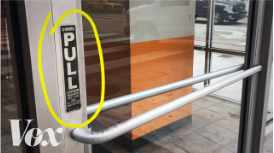
\includegraphics[scale = 0.7]{../immagini/sign.png}
	\caption{La scritta pull è un significante, data l'affordance della porta di essere spinta o tirata.}
\end{figure}
\begin{figure}[!h]
	\centering
	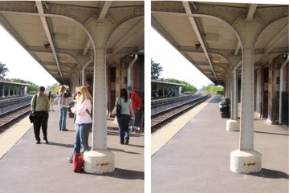
\includegraphics[scale = 0.7]{../immagini/sign1.png}
	\caption{Le persone che aspettano il treno sono un esempio di significante sociale.}
\end{figure}

\section{Mapping}
\textbf{Mapping} è un termine tecnico, ripreso dalla matematica, che indica la relazione fra gli elementi di due insiemi.

Il concetto di \textbf{mapping} è di grande importanza nella progettazione di interfacce, in particolare nel \textbf{posizionamento dei significanti}. La disposizione dei significanti può comunicare di più circa l'interfaccia e circa le sue funzionalità. Infatti se si sfrutta una corrispondenza spaziale fra la collocazione dei comandi e quella dei dispositivi comandati, risulta molto più facile capire come usarli.

Il modo migliore per \textit{fare} mapping è quello \textbf{naturale}, perché è un'attività in cui il cervello umano è molto bravo, i bambini imparano a fare mapping fin dai primi anni di vita. È da tenere presente che il concetto di \textbf{naturale} è ben diverso dal concetto di \textbf{universale}, poiché ci possono essere molti mappings che sembrano naturali ma che in realtà sono specifici a una cerchia di culture.

\begin{figure}[!h]
	\centering
	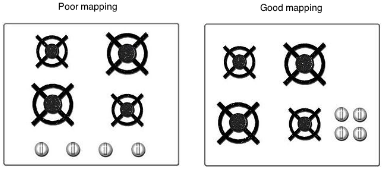
\includegraphics[scale = 0.7]{../immagini/mapping.png}
	\caption{Mapping cattivo e mapping buono.}
\end{figure}

\pagebreak

\section{Feedback}
Il feedback è la comunicazione del risultato di un'azione, è una risposta che l'interfaccia dà all'utente.

Il feedback \textbf{deve essere immediato}, anche un ritardo di un decimo di secondo può essere troppo, se il ritardo è troppo lungo l'utente potrebbe rinunciare all'attività che stava compiendo e passare ad altro o addirittura non riuscire a comprendere l'origine del feedback stesso.

\textbf{Deve essere informativo}, non deve portare con sè troppa informazione, ma deve assolvere al proprio obiettivo, deve far capire che un'azione è in corso o che è stato prodotto il risultato che ci si aspetta. Uno scarso feedback può essere peggio di nessun feedback, perché distrae, crea confusione e di conseguenza frustrazione nell'utente.

Un altro caratteristica importante è \textbf{la semplicità}, un feedback non deve essere pedante: troppi annunci o segnali portano le persone ad ignorarli perdendo anche i feedback cruciali e veramente importanti. Il feedback deve essere \textbf{essenziale} e mantenere l'ambiente calmo e tranquillo.

\section{Modello concettuale}
Un modello concettuale è una descrizione altamente semplificata delle funzionalità di un sistema, non deve essere completa o accurata ma \textbf{utile}. I file, le cartelle e le icone che si vedono sullo schermo del computer aiutano le persone a crearsi un modello concettuale dei dati in memoria o delle applicazioni disponibili. In realtà il computer non contiene fascicoli o cartelle: esse sono solo concettualizzazioni ideate per facilitarne l'uso.

\textbf{I modelli semplificati sono preziosi e utili fintanto che le ipotesi che li supportano sono vere.} Nel cloud storage i file sembrano essere sul dispositivo, ma in molti casi il materiale è in realtà nel cloud. Il modello concettuale veicolato è quello di un archivio disponibile sui dispositivi degli utenti. Questo modello semplificato è utile e basta per il normale utilizzo, ma se il collegamento dei servizi si interrompe, può nascere confusione nell'utente: l'informazione è sempre presente sullo schermo, ma egli non può più salvarla o recuperare altri dati, cosa inspiegabile in relazione al modello concettuale precedentemente veicolato.

Il modello concettuale esprime \textbf{come il designer vuole che l'utente percepisca il prodotto}, sarebbe, in un certo senso, l'ambizione di progettare e comprendere la UX. Una volta che i progettisti hanno pensato e progettato il modello concettuale si implementa l'interfaccia, in modo che il modello concettuale venga veicolato all'utente tramite affordances, significanti e mapping presenti su di essa.

Quando una persona interagisce con il sistema o con il prodotto sviluppa un suo modello mentale. Un \textbf{modello mentale} è un modello concettuale nella mente dell'utente che rappresenta il modo in cui, secondo lui, funzionano le cose. Non solo persone diverse possono avere modelli mentali diversi dello stesso oggetto, ma la stessa persona può avere molteplici modelli, pertinenti ciascuno ad un aspetto diverso del suo funzionamento, e persino contraddittori gli uni con gli altri.

\textbf{Più è grande la differenza tra il modello mentale e quello concettuale, più l'utente farà fatica ad usare il sistema.}

L'ideale è che l'utente apprenda un modello concettuale giusto \textbf{direttamente dal device che utilizza}, senza andare a leggere manuali o istruzioni o, peggio ancora, che gli venga trasmesso da terzi. La comprensione di un dispositivo tramite passaparola porta all'\textbf{effetto del telefono senza fili}: l'interpretazione cambia da persona a persona. Per questo vi è necessità che il modello concettuale trasmesso dal prodotto sia pressoché unico in relazione a quello mentale che l'utente si costruisce. In questo contesto vale l'affermazione \textit{less is more} secondo cui se una feature è difficile da veicolare allora è meglio non implementarla.

\pagebreak

\section{Immagine di Sistema}
Le persone si creano di continuo, attraverso l'esperienza, l'addestramento e l'istruzione, modelli mentali di sé, degli altri, dell'ambiente e degli oggetti con cui esse interagiscono.

Questi modelli servono agli uomini da guida per realizzare i loro scopi e comprendere il mondo in cui vivono.

Come fanno gli uomini a formarsi un modello concettuale adeguato dei dispositivi che utilizzano? Non potendo parlare con il progettista, essi si basano su tutta l'informazione accessibile: l'aspetto dell'apparecchio, cosa hanno imparato dall'uso di oggetti simili in passato, cosa comunicano le pubblicità, i venditori, i pieghevoli illustrativi, il sito web e il libretto di istruzioni.

\textbf{L'insieme di tutta questa informazione è l'immagine di sistema}.

\begin{figure}[!h]
	\centering
	\includegraphics[scale = 0.75]{"../immagini/Immagine di Sistema"}
\end{figure}

Come illustrato nella figura, il progettista e l'utilizzatore finale del prodotto costituiscono i vertici scollegati di un triangolo. Il vertice del triangolo più a destra è occupato dal modello concettuale del progettista, \textbf{cioè dalla sua concezione del prodotto in questione}.

Una volta commercializzato, il prodotto si stacca dal progettista: lo vediamo infatti isolato nel secondo vertice del triangolo.

\textbf{L'immagine di sistema è tutto ciò che si percepisce dalla struttura fisica prodotta, completa di documentazione, istruzioni,significanti e ogni informazione accessibile dal sito web o dal servizio di assistenza clienti}.

Il modello concettuale dell'utente deriva dall'immagine di sistema, mediante l'interazione con il prodotto, mediante letture, ricerche online e manuali. Il progettista si aspetta che il modello concettuale dell'utente coincida col suo, ma, non essendoci comunicazione diretta fra lui e l'utente, tutto il peso della comunicazione grava invece sull'immagine di sistema.

Questo spiega perché la comunicazione è un aspetto importante del buon design. \textbf{ Per quanto sia geniale il prodotto, se la gente non riesce ad usarlo l'accoglienza sarà cattiva}. Tocca al progettista fornire le informazioni adeguate per rendere il prodotto comprensibile ed usabile. Quel che più conta è presentare un modello concettuale capace di guidare l'utente quando le cose non vanno come dovrebbero.

Un buon modello concettuale è la chiave per avere prodotti comprensibili, di facile uso e gradevoli, e una buona comunicazione è importantissima per ottenere buoni modelli concettuali.

\pagebreak

 %Principi Fondamentali dell'Interazione
\section{Vincoli}
%\chapter{Constraints, Discoverability e Feedback}
\begin{flushleft}
	\textit{In che modo si riesce a capire una cosa che non abbiamo mai visto prima?}
\end{flushleft}

Non c'è altro da fare che combinare l'informazione presente nel mondo esterno con quella che si ha in testa.

L'insieme di conoscenze che si trovano nel mondo comprende le affordances, i significanti visibili, le corrispondenze fra quelle parti degli oggetti che sembrano comandi o punti da manipolare, le azioni risultanti e i vincoli fisici che limitano ciò che è possibile fare.

La conoscenza si ha in mente comprende i modelli concettuali, i vincoli culturali, semantici e logici del comportamento, le analogie fra la situazione attuale ed esperienze precedenti.

\begin{figure}[!h]
	\centering
	\includegraphics[scale = 0.7]{"../immagini/Modellino Lego"}
	\caption{Un modellino lego.}
\end{figure}

Si prenda come esempio il modellino Lego presente in figura: ha 15 pezzi, solo alcuni specializzati, molti altri sono di grandezza e forma uguale ma di colori diversi. Combinando i vincoli fisici con quelli culturali, semantici e logici si riesce a costruire il modellino senza istruzioni, mettendo ogni pezzo nella sua giusta posizione.

Vincoli fisici limitano le parti che possono andare insieme, i vincoli culturali e semantici impongono restrizioni precise a tutti i pezzi restanti e se rimane fuori qualche pezzo l'incastro è dettato dalla logica.

\textbf{I vincoli sono indizi potenti}, che limitano l'insieme delle azioni possibili. L'uso intelligente dei vincoli in sede di design permette alle persone di decidere prontamente il giusto corso d'azione, anche in una situazione del tutto nuova.

\pagebreak

È possibile categorizzare i vincoli in \textbf{quattro} classi:
\begin{itemize}
	\item \textbf{Vincoli fisici}: si affidano a proprietà del mondo fisico, senza alcun bisogno di istruzioni o di addestramento. Nell'esempio della motocicletta Lego ritroviamo questo vincolo nei pezzi che si incastrano solo in un determinato verso.
	\item \textbf{Vincoli culturali}: si affidano alle abitudini culturali, sociali, comportamentali che possono cambiare nel tempo. Con \textbf{vincolo culturale} s'intendono anche le convenzioni. Nell'esempio della motocicletta Lego ritroviamo questo vincolo nel saper determinare la collocazione delle luci: bianco all'anteriore e rosso al posteriore.
	\item \textbf{Vincoli semantici}: si affidano al significato della situazione per circoscrivere l'insieme delle azioni possibili, si basano sulla conoscenza della situazione e del mondo. Nel caso della motocicletta, c'è un'unica collocazione sensata per il motociclista, deve stare seduto guardando in avanti.
	\item \textbf{Vincoli logici}: dettati dalla semplice e pura logica umana. Se avanzasse un un solo pezzo per assemblare la motocicletta, grazie alla logica sapremo dove collocarlo nella sua giusta posizione.
\end{itemize}

Un buon designer può sfruttare questi vincoli per veicolare l'utente verso un modello mentale del prodotto che si avvicini il più possibile al modello concettuale desiderato ed in tal modo garantirgli una UX gradevole.

%\section{Vincoli e mapping}
Vincoli e mapping a volte si confondono tra di loro. Una serie di interruttori mappati in maniera opportuna infondono un vincolo logico che permette all'utente di non sbagliare, si intuisce perfettamente cosa verrà azionato da quell'interruttore posto in quel determinato punto. \textbf{Mapping forti possono diventare dei vincoli logici}.
L'assenza di vincoli e mapping genera, come già ribadito più volte, frustrazione poiché crea una interfaccia poco chiara e difficile da comprendere.
\begin{figure}[!h]
	\centering
	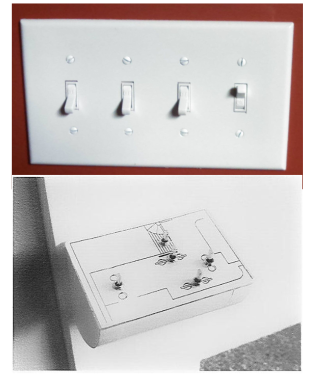
\includegraphics[scale=0.67]{../immagini/Interruttori}
	\caption{Un interruttore per le luci di una stanza che imita la piantina del locale.}
\end{figure}

\pagebreak

\section{Funzioni Obbliganti}
\textbf{Le funzioni obbliganti sono una forma di vincolo fisico}: consistono di situazioni in cui le azioni sono vincolate in modo che un passaggio mancato impedisca di procedere al successivo.

Sono il caso estremo di vincoli atti ad impedire un comportamento inappropriato.

Non tutte le situazioni permettono l'uso di vincoli così forti, ma il principio generale è applicabile negli ambiti più diversi.

Si esaminano ora tre di questi metodi:
\begin{itemize}
	\item \textbf{Interlock}: obbliga a eseguire una serie di operazioni (n maggiore di 1) nella sequenza dovuta prima di avviare l'azione richiesta. Gli interlock sono usati soprattutto come sistemi di sicurezza nei macchinari idnustriali ma anche nel mondo software come per esempio nel caso dei sistemi Captcha.
	
	\begin{figure}[!h]
	\centering
	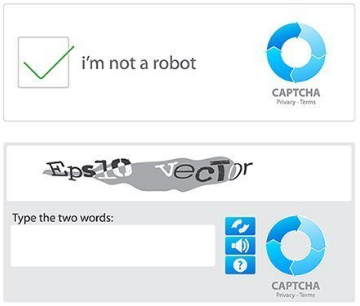
\includegraphics[width=0.4\textwidth]{../immagini/cap.png}
	\caption{I captcha sono un esempio di interlocks.}
\end{figure}

\begin{figure}[!h]
	\centering
	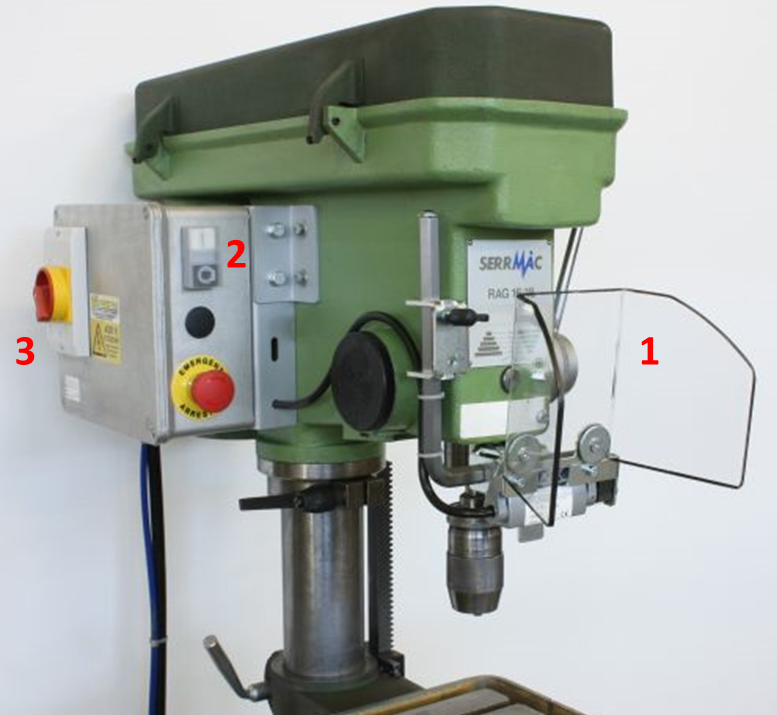
\includegraphics[width=0.5\textwidth]{../immagini/trapano.png}
	\caption{Per usare un trapano a colonna professionale è necessario 1) chiudere lo sportello di sicurezza; 2) armare il sistema premendo l'apposito bottone; 3) attivare il motore ruotando l'interruttore rosso. Se uno di questi passaggi viene ignorato il sistema non si attiva. Se una volta attivato il sistema, lo sportello viene aperto il motore si spegne. }
\end{figure}

	\item \textbf{Lock-in}: mantiene attiva una funzione impedendo che qualcuno la interrompa prematuramente. È usato molto in ambito informatico (e.g. ogni tentativo di uscita da un'applicazione senza salvare è prevenuto da un messaggio di allerta che chiede la conferma dell'intenzione). \textbf{Per finire un task si deve compiere un'azione.}
	
	\begin{figure}[!h]
	\centering
	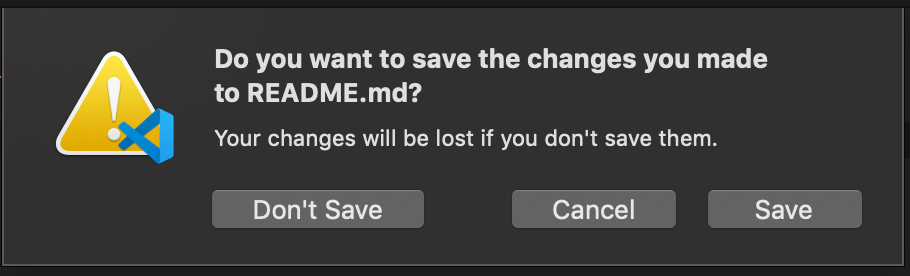
\includegraphics[width=0.4\textwidth]{../immagini/savedialog.png}
	\caption{Il dialog dove viene proposto di salvare prima di chiudere è un esempio di lock-in dal momento che blocca "dentro" il software l'utente fino a che questo non da un ulteriore input.}
\end{figure}


	\item \textbf{Lockout}: impedisce l'ingresso in uno spazio pericoloso o impedisce che succeda qualcosa. Può essere considerato l'opposto del lock-in. Un esempio di stampo informatico, sono gli \textbf{alert VM 18} che si possono trovare su alcuni siti. \textbf{Per accedere ad un task si deve compiere un'azione.}
\end{itemize}

	\begin{figure}[!h]
	\centering
	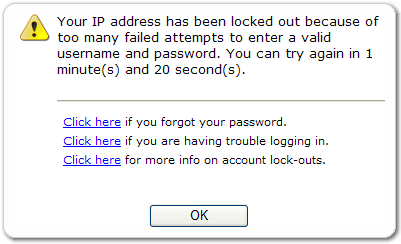
\includegraphics[width=0.5\textwidth]{../immagini/lockout.png}
	\caption{Bloccare un utenza perchè ha immesso troppe volte credenziali sbagliate è un esempio di lock-out. Per superare il blocco bisogna attendere o seguire delle specifiche procedure.}
\end{figure}



\section{Activity-Centered Control}
Il mapping spaziale dei comandi non sempre è il più opportuno.

In molti casi è meglio avere interruttori diversi per attività diverse: \textbf{comandi centrati sulle attività}.

Azionando un semplice comando si impostano una serie di oggetti per svolgere una determinata attività, senza comandarli uno ad uno. In molti auditorium ci sono interruttori con indicazioni \textit{video}, \textit{computer}, \textit{piena luce} e \textit{lezione} che impostano il microfono, le luci della sala, il proiettore e quant'altro.

Questo schema è eccellente in teoria, ma nella pratica è difficile da realizzare bene, soprattutto è necessario valutare gli \textbf{imprevisti} e le possibili risoluzioni.

Per carità, il metodo è giusto, purché la gamma di attività sia scelta in modo da corrispondere alle situazioni reali. Ma anche in quel caso saranno pur necessari dei comandi manuali, perché si presenteranno sempre esigenze inattese, che richiederanno una regolazione particolare dei dispositivi.

La Logitech ha prodotto una serie di telecomandi universali completamente progettati attorno al concetto degli Activity Centereed Control \url{https://www.logitech.com/it-it/harmony-universal-remotes}.

	\begin{figure}[!h]
	\centering
	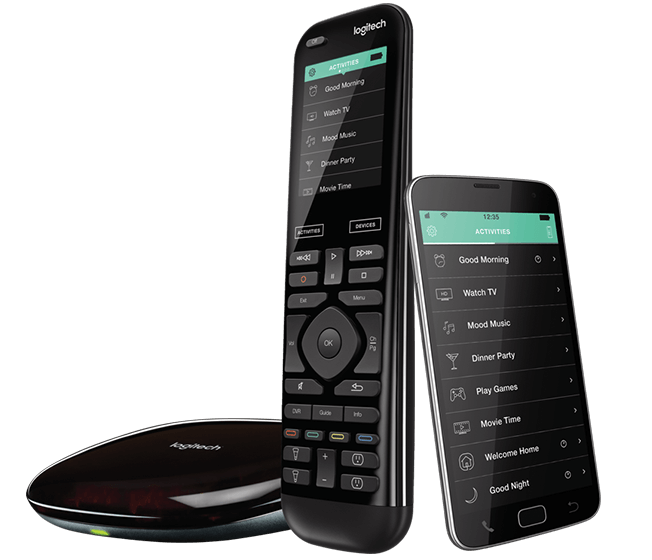
\includegraphics[width=0.5\textwidth]{../immagini/harmony.png}
	\caption{Il telecomando universale Harmony di Logitech consente di controllare vari dispositivi attraverso un modello di interazione basato sugli activity centered controls. Non si seleziona più il dispositivo che si vuol controllare ma l'attività che si vuol fare: Play Game, Watch TV, etc..}
\end{figure}
 %Constraints, Discoverability e Feedback
%\chapter{How do people do things}
\begin{flushleft}
	\textit{
		È facile imparare alcune azioni elementari per far funzionare un dispositivo tecnico. Ma cosa succede se le cose non vanno come dovrebbero? Come può l'utente accorgersene, e scoprire cosa fare? }
\end{flushleft}

Per chiarire meglio tutto questo è bene soffermarsi prima sulla psicologia umana e sui modi con cui gli uomini scelgono e valutano le proprie azioni. Fatto ciò si passerà a esaminare il ruolo della cognizione e delle emozioni in tale processo: il piacere quando le cose funzionano senza intoppi e la frustrazione quando le aspettative iniziali degli utenti non sono realizzate.

\section{I Golfi dell'Esecuzione e della Valutazione}
Quando usiamo un oggetto, ci si trova davanti due golfi: il \textbf{golfo dell'esecuzione}, nel quale si cerca di indovinare cosa fare, e il \textbf{golfo della valutazione}, in cui ci si sforza di capire cosa è successo. Il compito del progettista è quello di aiutare gli utenti a superare i due golfi e renderli il meno profondi possibili.

\begin{figure}[!h]
	\centering
	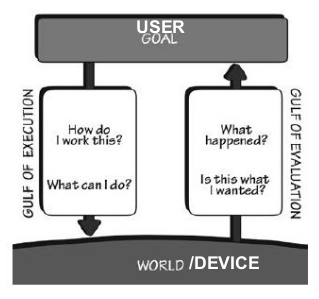
\includegraphics[scale=0.73]{immagini/Golfi}
	\caption{Golfo dell'esecuzione e golfo della valutazione.}
\end{figure}

Il \textbf{golfo della valutazione} corrisponde allo sforzo necessario per interpretare lo stato fisico del dispositivo e capire fino a che punto sono state realizzate le aspettative e le intenzioni iniziali. Il Golfo è stretto quando il dispositivo fornisce informazioni sul proprio stato, in una forma facile da cogliere e interpretare.

\pagebreak

\begin{flushleft}
	\textit{
		Quali sono gli elementi progettuali più importanti per superare il golfo della valutazione?}
\end{flushleft}

Il \textbf{feedback} e un \textbf{modello concettuale adeguato}.

\begin{flushleft}
	\textit{Quali sono gli elementi progettuali più importanti per superare il golfo dell'esecuzione?}
\end{flushleft}
\textbf{Significanti}, \textbf{constraints}, \textbf{buon mapping} e un modello concettuale adeguato.

Entrambi i golfi sono presenti in molti apparati. Si incontrano spesso difficoltà, puntualmente liquidate accusando sè stessi. Di fronte alle difficoltà nell'uso di congegni che ci si aspetta di saper usare si finisce inevitabilmente col pensare di essere stupidi. Oppure, con dispositivi dall'aspetto più complicato, semplicemente ci si arrende, pensando di essere incapaci di utilizzarli. Queste spiegazioni sono entrambe sbagliate. \textbf{Le difficoltà hanno origine nel design, non nell'utente}.

\section{I sette stadi dell'azione}
Compiere un'azione implica due fasi: \textbf{esecuzione e valutazione degli effetti}, \textbf{fare e interpretare}. Sia l'esecuzione che la valutazione richiedono che si capisca come funziona l'oggetto su cui si applica l'azione e quali risultati essa produce. Entrambe le fasi influiscono sullo stato emotivo dell'utente.

Un progettista deve conciliare il compito che l'utente vorrebbe eseguire e tutte le possibili azioni fisiche che può compiere per eseguirlo. Una volta che l'utente specifica quali azioni compiere, bisogna far in modo le esegua concretamente: ciò costituisce lo \textbf{stadio dell'esecuzione}. \textbf{Identificato il goal, o scopo, l'utente discende attraverso i tre stadi dell'esecuzione: pianificare, specificare ed eseguire.}

\textbf{La valutazione si articola anch'essa in tre stadi: percepire, interpretazione, confrontare.}

Ecco così che si hanno i \textbf{sette stadi dell'azione}: uno per lo scopo, tre per l'esecuzione e tre per la valutazione.
\begin{itemize}
	\item \textbf{Scopo}: definire l'obiettivo.
	\item \textbf{Progettare}: definire l'azione da eseguire.
	\item \textbf{Specificare}: costruire una sequenza d'azione.
	\item \textbf{Eseguire}: eseguire la sequenza specificata.
	\item \textbf{Percepire}: osservare lo stato del mondo.
	\item \textbf{Interpretare}: elaborare la percezione.
	\item \textbf{Confrontare}: rapportare il risultato allo scopo.
\end{itemize}
\begin{center}
	\includegraphics[width=0.5\linewidth]{"immagini/Sette stadi"}
\end{center}
La maggior parte delle azioni non richiede che si percorrano tutti i sette stadi in sequenza, ma quasi nessuna attività si risolve in tramite un'azione singola.

Di solito si applicano numerose sequenze e l'intera attività può durare ore o giorni. Ci sono molteplici circuiti di feedback, con cui i risultati di un'attività vengono usati per indirizzare l'utente verso altre, in cui uno scopo genera scopi accessori e ogni un progetto sotto-progetti. Ci sono attività in cui lo scopo originario è addirittura dimenticato, scartato o riformulato.

I sette stadi offrono uno schema per sviluppare nuovi prodotti o servizi. I golfi dell'esecuzione e della valutazione sono i punti più ovvi da cui partire, offrendo entrambi spunti per migliorare il prodotto. I progettisti devono svilupparne capacità di osservazione.

\section{Tre livelli di Processing}
Gli stadi dell'azione possono essere associati a tre livelli di processing mentale: viscerale, comportamentale e riflessivo.

\begin{itemize}
	\item \textbf{Livello viscerale}: è il livello più elementare, permette di rispondere prontamente in maniera subconscia, senza consapevolezza o controllo cosciente.
	\item \textbf{Livello comportamentale}: è la sede delle abilità apprese durante circostanze più o meno simili a quelle attuali. Durante l'esecuzione, il livello comportamentale è guidato dalle aspettative, e durante l'attesa di conferma di tali aspettative è invece guidato dalle emozioni. Il livello comportamentale stabilisce in che modo si compie una determinata azione e in che modo si interpreta un determinato feedback.
	\item \textbf{Livello riflessivo}: è il livello della cognizione conscia, è qui che si sviluppa la comprensione profonda e hanno luogo il ragionamento e i processi decisionali. Qui fanno capo i livelli più alti di emotività: soddisfazione e orgoglio, ma anche frustrazione e senso di colpa.
\end{itemize}

\begin{figure}[!h]
	\centering
	\includegraphics[scale=1]{"immagini/Livelli di Processing"}
\end{figure}

\pagebreak

\textbf{Veicolare informazioni all'utente mentre egli si trova nel livello riflessivo è estremamente efficace}. Al livello riflessivo il suo pensiero è conscio e le emozioni che egli produce sono le più durature.

Gli stimoli riflessivi sono parte integrante del ricordo degli eventi, è importante quindi creare nell'utente ricordi positivi mentre egli è in questo stadio dell'azione, perché tali ricordi sono i più duraturi.

Inoltre è la riflessione, intesa come pensiero cosciente, che induce a consigliare un prodotto e raccomandarne l'uso o magari a sconsigliarlo.

I tre livelli di elaborazione contribuiscono tutti insieme a determinare lo stato emotivo e cognitivo dell'utente. Funzioni riflessive di alto livello possono mettere in moto emozioni più elementari e  queste, a loro volta, possono stimolare attività cognitive di tipo riflessivo.

\section{I sette Principi Fondamentali della Progettazione}
Il modello a sette stadi del ciclo d'azione è un prezioso sussidio per il design, in quanto introduce una lista di domande fondamentali. In generale, ogni stadio dell'azione richiede specifiche strategie progettuali, e, viceversa, presenta occasioni proprie di disastro.

Ne derivano dunque sette domande, a cui dovrebbe poter rispondere chiunque stia usando un determinato prodotto.

\begin{itemize}
	\item \textbf{Cosa voglio ottenere?}
	\item \textbf{Quali sono le sequenze d'azione alternative?}
	\item \textbf{Quale azione posso fare ora?}
	\item \textbf{Come faccio questa azione?}
	\item \textbf{Cosa è successo?}
	\item \textbf{Cosa significa?}
	\item \textbf{Va bene? Ho realizzato il mio scopo?}
\end{itemize}

\begin{figure}[!h]
	\centering
	\includegraphics[scale=0.55]{"immagini/Sette Domande"}
\end{figure}

\pagebreak

Il progettista ha la responsabilità di garantire che a ogni stadio dell'azione il prodotto fornisca l'informazione necessaria per proseguire correttamente.

L'informazione che serve a rispondere alle domande nelle fasi attuative è definita come \textbf{feedforward}.

L'informazione che aiuta a capire quello che è successo nella fasi percettive è definita invece come \textbf{feedback}.

Il \textbf{feedforward} si realizza mediante l'uso opportuno di significanti, vincoli e mapping, anche il modello concettuale ha un ruolo importante.

Il \textbf{feedback} è dato dall'immediato cambiamento di stato che il prodotto deve mostrare all'utente e, anche qui, una parte importante è svolta dal modello concettuale.

Sia il \textbf{feedback}, che il \textbf{feedforward} devono presentarsi in una forma facilmente interpretabile da chi utilizza il sistema. La presentazione deve corrispondere alla visione che le persone hanno dello scopo che vogliono realizzare e alle loro aspettative. L'informazione erogata deve essere immediatamente comprensibile.

Dalle risposte relative ai sette stadi dell'azione si ricavano sette principi fondamentali del design:

\begin{itemize}
	\item \textbf{Visibilità}: è bene che sia facile scoprire immediatamente quali azioni sono possibili e qual è lo stato attuale del dispositivo.
	\item \textbf{Feedback}: è opportuno che ci sia un'informazione completa e continua riguardo ai risultati delle azioni e allo stato attuale del prodotto o del servizio. Dopo aver eseguito un'azione, deve essere facile determinare il risultato.
	\item \textbf{Modello Concettuale}: il design dovrebbe fornire tutta l'informazione necessaria per creare un buon modello concettuale del sistema, che favorisca la comprensione e la sensazione di controllo da parte dell'utente. Il modello concettuale potenzia sia la visibilità, sia la valutazione dei risultati.
	\item \textbf{Affordance}: è bene che le affordance siano fatte apposta per rendere possibili le azioni desiderate e impossibili quelle indesiderate.
	\item \textbf{Significanti}: un uso efficace dei significanti assicura la visibilità e la comprensibilità dei comandi.
	\item \textbf{Mapping}: è necessario che la relazione fra i comandi e le rispettive azioni obbedisca ai principi del buon mapping, sostenuto, per quanto possibile, dalla disposizione spaziale e dalla contiguità temporale.
	\item \textbf{Vincoli}: bisogna fornire vincoli fisici, logici, semantici e culturali, in modo tale da guidare l'azione e facilitandone l'interpretazione.
\end{itemize}
Questi sette principi sono mappati uno ad uno sugli stadi d'azione dell'utente.

È bene concludere con una nota la parte dedicata a strumenti, metodi ed elementi per il design dello human-computer interaction: per molte attività quotidiane , gli obiettivi e le interazioni non sono ben definiti, \textbf{sono più di tipo opportunistico che frutto di una pianificazione}.

Le azioni opportunistiche sono quelle in cui il comportamento scaturito dalle circostanze prevale sulla pianificazione. Gli utenti in questi casi agiscono in maniera non controllata e quindi non prevedibile.

È difficile fare buon design per queste situazioni, anche attenendosi a tutti i principi esposti fino ad ora: l'utente che agisce in maniera opportunistica romperà in ogni caso questi schemi.

\pagebreak
 %How do people do things
%\chapter{Metodi e Strumenti per l'Innovazione}

Introduciamo ora una serie di metodi di lavoro e strumenti nati per facilitare la progettazione e realizzazione di prodotti e sistemi innovativi. 

\begin{flushleft}
\textit{ \textbf{Innovazióne} s. f. [dal lat. tardo innovatio -onis]. L’atto, l’opera di innovare, cioè di introdurre nuovi sistemi, nuovi ordinamenti, nuovi metodi di produzione. In senso concreto, ogni novità, mutamento, trasformazione che modifichi radicalmente o provochi comunque un efficace svecchiamento in un ordinamento politico o sociale, in un metodo di produzione, in una tecnica, ecc. [Treccani]}
\end{flushleft}

In innovazione, l'applicazione della filosofia HCD diventa di vitale importanza dal momento che un prodotto o servizio per essere innovativo deve essere prima di tutto apprezzato dagli utenti e quindi utilizzato.

\textbf{Cosa vuol dire innovare? Esiste un solo modo di fare innovazione?}

\section{Disruptive Innovation}
\begin{flushleft}
	\textit{\textbf{People don’t want to buy a quarter-inch drill. They want a quarter-inch hole!} - Professor Theodore Levitt, Harvard Business School}\\

\end{flushleft}

La maggior parte dell'innovazione è fatta come miglioramento incrementale di prodotti o sistemi già esistenti. I nuovi condizionatori d'aria, per esempio, hanno motori e gas più efficienti rispetto al passato ma il loro funzionamento è basato sul principio della macchina frigorifera che fu proposto per la prima volta nel 1835.
Questo approccio all'innovazione fatta attraverso piccole migliorie apportate ad un sistema stabile è il più comune. Questo processo passo-passo è molto affidabile, consente di raggiungere buoni risultati con investimenti tutto sommato contenuti e di mantenere invariata la struttura delle aziende (produttori) e della società (consumatore). Questo processo di innovazione incrementale ha però bassissime probabilità di portare ad una modifica sostanziale del prodotto/processo su cui è applicato.

L' \textbf{innovazione incrementale} punta infatti al mantenimento della competitività aziendale tramite un processo passo-passo dove si fa un aggiornamento alla volta. Nel paradigma di innovazione incrementale la clientela di riferimento è stabile e definita e non si punta solitamente ad espandere il business verso altre nicchie di clientela.

In generale però, quando si parla di innovazione, ci si aspetta di trovarsi davanti ad un prodotto o servizio che cambi radicalmente il modo in cui si fanno le cose. Qualcosa di nuovo, destinato a ``cambire il mondo''. Questo tipo di innovazione è detto \textbf{disruptive innovation} e si basa su una forte discontinuità con il passato. L'innovazione di tipo dirompente è spesso alla base dei modelli di business e di sviluppo delle startup ed è uno degli elementi di differenziazione che c'è fra una startup e un'impresa tradizionale.

Il termine \textit{disruptive innovation} è stato utilizzato per la prima volta da Clayton Christensen nel libro ``Il dilemma dell’innovatore'' del 1997 per spiegare come i processi innovativi attuati dalle aziende seguano principalmente due paradigmi.

Nella \textbf{disruptive innovation}, si punta quindi a conquistare quelle nicchie di clientela che risultano ancora irraggiungibili tramite i prodotti, le tecnologie e i sistemi esistenti. Per fare questo si mette in discussione l'intero impianto tecnologico e di business del prodotto e si ridisegna il tutto sulla base delle moderne tecnologie così da cercare di acquisire nuovi mercati inesplorati e quindi più fertili.

È sempre molto difficile definire a posteriori quale prodotto o tecnologia è/sia stato disruptive e quale no. I prodotti, i sistemi e le tecnologie diventano ovvie un secondo dopo che sono state accettate dal mercato e quindi ci si dimentica velocemente di come questi abbiano cambiato il mondo in cui viviamo. 

Si ha innovazione dirompente quando un prodotto è in grado di offrire performance e possibilità di utilizzo completamente impensabili rispetto alle precedenti soluzioni o di definire un mercato di riferimento completamente nuovo.

Un indiscutibile esempio di innovazione dirompente è sicuramente stato \textbf{Internet}. Grazie alla Rete sono nati sistemi di comunicazione, modelli di business, prodotti e culture che prima non esistevano. Internet ha cambiato il mondo in una maniera così radicale da non consentire un ritorno al passato. È indubbio che oggi sarebbe impossibile vivere senza rete.

Il settore dove invece regna sovrana l'innovazione incrementale è sicuramente quello dell'automotive. Ogni anno escono auto che consumano un pochino meno, che sono un pochino più spaziose, comode e preformanti dei modelli precedenti ma la tecnologia che sottostà questo processo è sempre la stessa. Il primo brevetto di un motore a combustione interna è del 1853 e da allora i suoi principi di funzionamento non sono mai stati modificati radicalmente ma solo ottimizzati ed evoluti.
Ma la disruptive innovation sta arrivando anche nel settore dell'automotive e nel giro di pochi anni le auto a guida autonoma e le motorizzazione elettriche diventeranno ovvie e il mondo dei trasporti non sarà più quello di una volta. Ci troveremo da un giorno all'altro a considerare ciò che ieri era fantascienza una nuova ovvia normalità e a considerare ciò che ieri era la norma preistoria.

A questo link (\url{http://www.concept.by/approfondimenti/innovazione-radicale/}) potete trovare un'interessante sintesi del libro ``Il dilemma dell'innovatore'' in cui per spiegare il concetto di innovazione dirompente è riportata la storia degli hard disk da 3,5 pollici.

La disruptive innovation è quindi il campo di gioco delle startup e di tutti quegli innovatori che lavorano per proporre nuovi modelli di business innovativi capaci di scalare rapidamente e globalmente. Non è un caso che aziende di successo, un tempo startup, come Airbnb, Amazon, Google, Facebook e Tesla tra le più recenti, ma anche le più longeve come Apple e Microsoft abbiano profondamente innovato i propri mercati in modo dirompente ed oggi rappresentino per tutti il concetto di innovazione. 

\begin{figure}[!h]
	\centering
	\includegraphics[width=\textwidth]{"immagini/Disruptive Innovation"}
		\caption{Sustaining e Disruptive innovation a confronto. Fonte: https://hcldr.wordpress.com/2017/01/10/disruptive-innovation-in-healthcare/}
\end{figure}

\textbf{Non si può fare innovazione dirompente senza una forme di pensiero e progettazione antropocentrica.}\\
Che vogliate cambiare il mondo dei trasporti (Uber, Tesla), andare su Marte (SpaceX), cambiare il modo in cui si sviluppano i servizi web (AWS, Microsoft Azure) o cambiare il modo in cui si va in vacanza (AirBnB, Booking) prima o poi il vostro prodotto o servizio avrà un utente, un acquirente, un finanziatore e un fan. Se non vi curerete di loro fin dalle prime fasi di progettazione la vostra sarà un'azione dirompente solo per voi stessi (e per il vostro portafoglio) perché un prodotto o servizio che nessuno utilizza non fa innovazione.

\section{Human Centered Design Process}
IDEO, una delle più grandi agenzie di design al mondo ha deciso di adottare lo Human Centerd Design in ogni suo progetto. IDEO ha inoltre creato intorno ai principi dello HCD una serie di strumenti di sviluppo e design che sono diventati molto popolari nel mondo del design di prodotto.

In particolare, IDEO ha proposto un vero e proprio metodo di progettazione basato sui fondamenti dell'HCD: lo \textbf{Human Centered Design Process}.

Se lo Human Centered Design pone l'accento sul fattore umano, lo Human Centered Design Process considera l'attività umana come un ombrello al di sotto del quale interagiscono i fattori umani, tecnologici e sociali.
Pertanto, rispetto ad un processo ``tradizionale'', lo Human Centered Design Process può essere definito come: \textit{``Un processo ispirato da comportamenti piuttosto che dalle statistiche, che si svolge in un contesto naturale piuttosto che in un ambiente controllato, e si basa su conversazioni aperte piuttosto che su interviste trascritte''}

Tutto questo processo, che potrebbe apparire astratto, in realtà poggia su un solido e preciso percorso di progettazione diviso in 3 fasi: Ispirazione, Ideazione e Implementazione.

\textbf{L'ispirazione}, la scoperta, sono legate all'osservazione dell'utente e dei suoi bisogni. Per IDEO, ad esempio, si tratta di capire come migliorare uno strumento osservando il modo in cui la persona utilizza quello strumento.  Quindi il risultato che ne verrà fuori sarà un design legato alla realtà dei fatti e delle situazioni e non alle ipotesi dei progettisti.

\textbf{L'ideazione} si basa sui contenuti appresi durante la fase dell'osservazione. Questi vengono messi in discussione e affrontati in gruppo, un'interazione da più ambiti in cui l'obiettivo è quello di ragionare su più idee possibili rimanendo focalizzati sui bisogni e le necessità dei destinatari. Da concetti ideali, come quelli della prima fase, si cerca di interpretare le conoscenze assunte per arrivare a qualcosa di più tangibile, magari tramite la creazione di un semplice prototipo. 

Il prototipo non deve essere definitivo né perfetto o completo di tutte le funzionalità necessarie. Serve come punto di partenza per un confronto con i destinatari del progetto. Non è un primo, vago tentativo di soluzione, ma fa sì che le risposte future risponderanno alle esigenze del target.

Incamerato il feedback, sarà più semplice continuare a testare e confrontarsi per arrivare all'attesa soluzione, senza inciampare lungo il cammino per arrivare alla fase di \textbf{implementazione}.

Ciascuna di queste fasi viene svolta dal team con un approccio a fisarmonica. All'inizio si lavora per produrre idee e soluzioni in quantità (divergenza), ci si focalizza poi nella selezione, fusione e integrazione delle proposte così da distillare i risultati e produrre un numero ridotto di soluzioni (convergenza) da passare alla fase successiva.

Video di presentazione dello HCD Process di IDEO: \url{https://vimeo.com/106505300}.

\begin{figure}[!h]
	\centering
	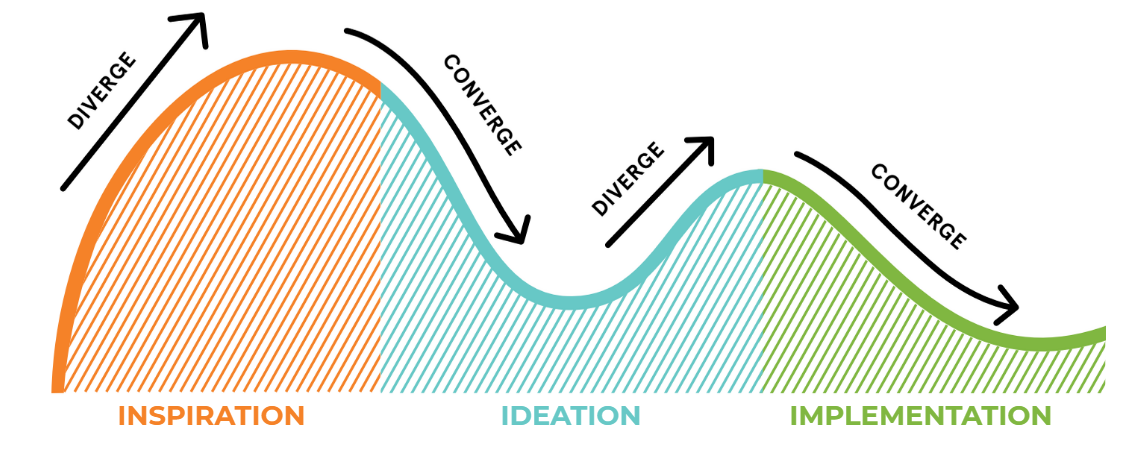
\includegraphics[width=0.8\textwidth]{immagini/HCD-process.png}
	\caption{HCD process. é un processo diviso in 3 fasi dove è sempre applicato un metodo di lavoro a fisarmonica che prevede una fase di divergenza e una di convergenza. Fonte https://blog.movingworlds.org/human-centered-design-vs-design-thinking-how-theyre-different-and-how-to-use-them-together-to-create-lasting-change/} 
	\label{hcd-process}
\end{figure}

\section{Design Thinking}
Il Design Thinking è un approccio all’innovazione che poggia le sue fondamenta sulla capacità di risolvere problemi complessi utilizzando una visione e una gestione del progetto basata sulla creatività. 

Tale approccio è stato codificato attorno agli anni 2000 in California dall’Università di Stanford. È centrato sulle persone (antropocentrico) e si basa sull’abilità di integrare capacità analitiche con attitudini creative. In genere viene applicato da un team multidisciplinare che ha come obiettivo quello di trovare una soluzione innovativa ad un problema (disruptive) tenendo conto del gradimento (human-centered) di essa, della redditività indotta e della sostenibilità economica (business).

In origine, il Design Thinking nacque come approccio all’innovazione adottato da agenzie e studi di design. Oggi invece, la sua diffusione sta permeando in settori molto diversi, anche in quelli ritenuti più distanti, fino a qualche anno fa. Il design thinking sta diventando infatti uno dei metodi di riferimento utilizzati dalle startup e da aziende innovative per la realizzazione di prodotti tecnologici, per la trasformazione digitale e la progettazione di software e interfacce.

Il DT ha 3 obiettivi fondamentali:

\begin{enumerate}
    \item avvicinarsi al cliente;
    \item favorire la creatività e generare idee;
    \item sperimentare rapidamente le idee attraverso la realizzazione di prototipi.
\end{enumerate}

Tuttavia ridurre il DT all’elenco degli obiettivi, dei settori di utilizzo o dei tool che lo caratterizzano è estremamente limitante. È invece molto più efficace ed importante comprendere il mindset e la prospettiva che caratterizzano i processi di DT. Questo perché, quotidianamente vengono proposti nuovi metodi, strumenti e tecnologie a supporto di questa modalità di progettazione e pertanto andare a trattarla sulla base degli strumenti più utilizzati è scorretto e limitante.

Relativamente all'approccio DT, Roberto Verganti Professore di Leadership and Innovation alla Stockholm School of Economics afferma: \textit{Si tratta di ribaltare il classico triangolo, tipico delle business school, che pone nel vertice in alto il business e alla base people e technology, a indicare come l’obiettivo dell’impresa sia l’uso dell’innovazione per creare business value a favore degli stakeholder, grazie a prodotti che soddisfino i bisogni delle persone attraverso l’uso delle tecnologie.} figura \ref{fig:dt_piramide}.

\textbf{L’approccio Design Thinking pone nel vertice in alto le persone.}

\textit{Partiamo dai sogni e dai problemi delle persone e creiamo prodotti che li soddisfino. Se ci riusciremo lo sviluppo del business ne sarà la naturale conseguenza.} 

In un processo di sviluppo basato su design thinking il business e la tecnologia sono solo degli strumenti per raggiungere l'obiettivo primo, la soddisfazione dell'utente.

\begin{figure}[!h]
	\centering
	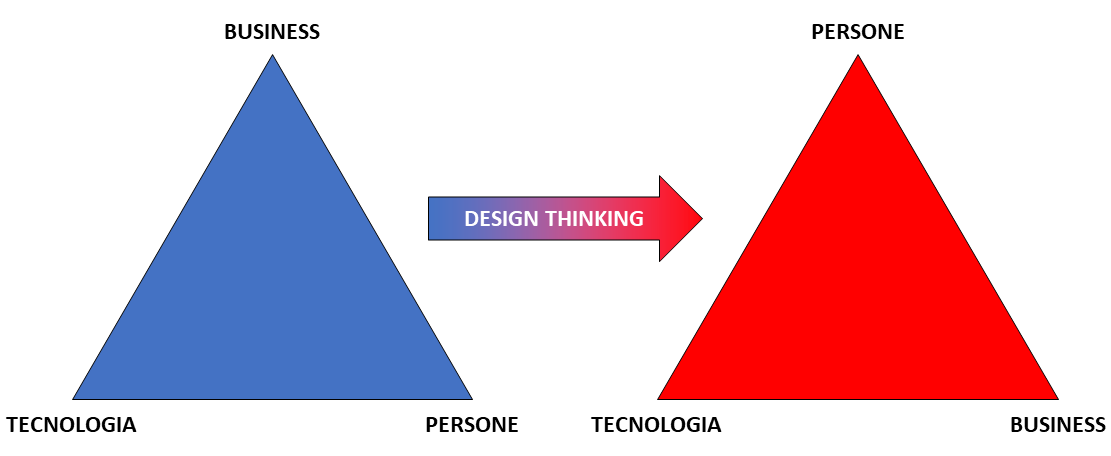
\includegraphics[width=\textwidth]{immagini/des_think.png}
	\caption{Nel design thinking gli obiettivi della progettazione cambiano radicalmente. L'elemento di riferimento diventa l'utente e la sua soddisfazione, il business e la tecnologia sono solo degli strumenti per raggiungere questo obiettivo.}
	\label{fig:dt_piramide}
\end{figure}

Questo diverso approccio assegna al termine design un significato nuovo, evidenziato del teorico del design Klaus Krippendorf che riporta il termine all’etimologia latina “de-signare”, e cioè, far si che qualcosa si distingua attraverso un segno, dandogli un significato. 

Il processo di sviluppo mediante Design Thinking può essere suddiviso in 5 fasi principali:

\begin{itemize}
	\item \textbf{Empathize}: La prima fase consiste nell’identificazione del problema e quindi dell’obiettivo; 
	\item \textbf{Define}: La seconda fase è orientata a delineare meglio le domande chiave, cioè quali sono i bisogni degli utenti e quindi quali sono le varie categorie di utenti;
	\item \textbf{Ideate}: La terza fase è quella orientata alla ricerca della soluzione, dell'opportunità tecnologica. In questa fase si fa uso di tecniche di stimolazione della creatività come brainstorming etc.;
	\item \textbf{Prototype}: La quarta fase è orientata alla realizzazione dei primi prototipi. Questa fase è molto importante per garantire un processo antropocentrico consentendo di andare il più velocemente possibile a testare il prodotto sul campo con gli utenti reali;
	\item \textbf{Test}: In fine la quinta fase è quella dedicata al test sul campo dei prototipi e alla raccolta dei feedback dagli utenti. Questa fase apparentemente conclusiva in realtà produce come output una serie di input per i futuri cicli di iterazione che si vanno ad applicare a tutte le fasi precedenti.
	
\end{itemize}

\begin{figure}
	\centering
	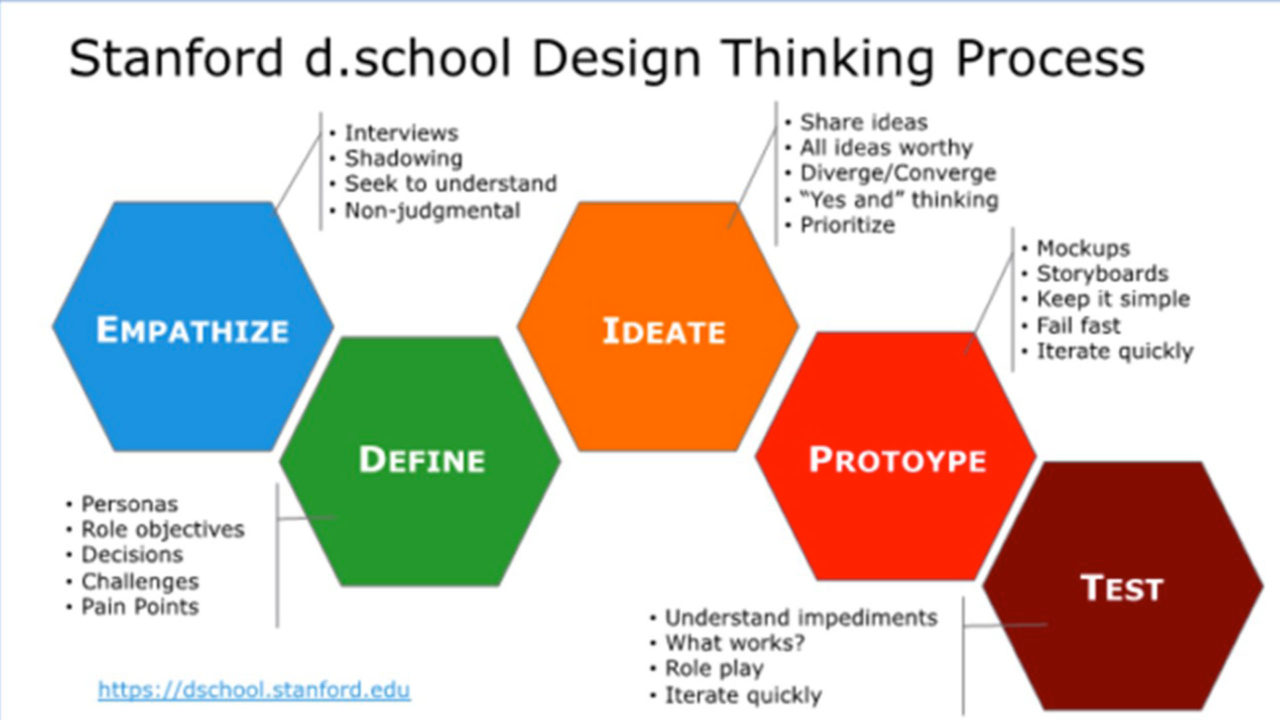
\includegraphics[width=\textwidth]{immagini/designthinking}
	\caption{Le 5 fasi del metodo Design Thinking. Fonte: https://www.zerounoweb.it/cio-innovation/metodologie/design-thinking-definizione-esempi/}
\end{figure}


Lo Human Centered Design è quindi un \textbf{mindset}, un modo di pensare e di approcciarsi allo sviluppo di prodotti. Come nel caso dello HCD Process, il Design Thinking, è invece un vero e proprio metodo di lavoro organizzato per fasi che consente di sviluppare prodotti centrati sull'utente grazie a tecniche orientate alla stimolazione della creatività e alla produzione di idee. Pensare di avviare un processo di disruptive innovation senza curarsi di progettare in maniera antropocentrica e senza un metodo di progettazione strutturato è al giorno d'oggi impossibile.

\begin{figure}
	\centering
	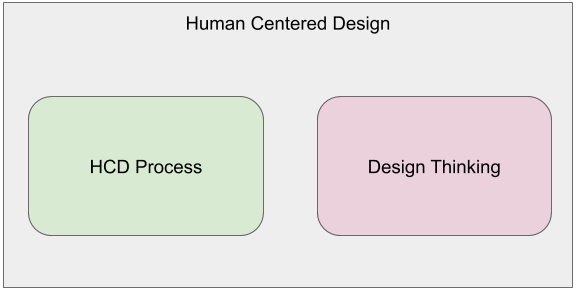
\includegraphics[width=0.6\textwidth]{immagini/dtvshcdp}
	\caption{HCD è una forma di pensiero, un approccio alla progettazione. HCD Process e Design Thinking sono invece metodi di progettazione molto utilizzati per il design di prodotti “disruptive”
}
\end{figure}

\section{Agile, Scrum e DevOps}
Nel mondo dello sviluppo software e dell'informatica in generale, negli ultimi anni si sono sviluppati molti metodi di organizzazione del lavoro orientati allo sviluppo veloce di sistemi innovativi. Tanti di questi metodi si basano su un mix di teorie e approcci di design applicati in altri settori e in generale puntano a dare al team di sviluppo un metodo di lavoro più snello, veloce e sopratutto orientato al prodotto e all'utente (antropocentrico).

% ---- Ridondanza? ----
%Il metodo di sviluppo software classico, presentato come fondamento dell'ingegneria del software è sicuramente il modello Waterfall.

In ingegneria del software, il modello a cascata (waterfall model in inglese) o ciclo di vita a cascata (waterfall lifecycle) è il più tradizionale modello di ciclo di vita del software. Secondo questo modello, il processo di realizzazione del software è strutturato in una sequenza lineare di fasi o passi, che comprende:

\begin{itemize}
    \item analisi dei requisiti
    \item progettazione
    \item sviluppo
    \item collaudo
    \item manutenzione

\end{itemize}

Questo modello riprende la sequenza di passi tipica della produzione manifatturiera, e fu il primo a essere applicato all'informatica quando lo sviluppo del software cominciò a essere concepito come attività industriale. Questo modello è stato progressivamente abbandonato dall'industria del software, ma rimane un importante riferimento storico.

Uno dei nuovi modelli di organizzazione dello sviluppo software che negli ultimi anni sta riscuotendo maggior successo è sicuramente l’Agile. Il metodo Agile nasce nel 2001 da un gruppo di 17 sviluppatori, che sentirono il bisogno di ripensare il loro modo di lavorare perché stufi del classico metodo di sviluppo waterfall. 
L'obiettivo di questi sviluppatori era quello di progettare un nuovo metodo di lavoro orientato allo sviluppo di applicazioni software in maniera più leggera, economica e rapida. 




\begin{figure}[h!]
	\centering
	\includegraphics[width=\textwidth]{"immagini/agile_manifesto"}
\end{figure}

Produssero quindi un manifesto a partire dal quale sono stati sviluppati i 12 principi fondamentali dell'Agile:

\begin{enumerate}
    \item Our highest priority is to satisfy the customer
through early and continuous delivery
of valuable software.

\item Welcome changing requirements, even late in
development. Agile processes harness change for
the customer's competitive advantage.

\item Deliver working software frequently, from a
couple of weeks to a couple of months, with a
preference to the shorter timescale.

\item Business people and developers must work
together daily throughout the project.

\item Build projects around motivated individuals.
Give them the environment and support they need,
and trust them to get the job done.

\item The most efficient and effective method of
conveying information to and within a development
team is face-to-face conversation.

\item Working software is the primary measure of progress.

\item Agile processes promote sustainable development.
The sponsors, developers, and users should be able
to maintain a constant pace indefinitely.

\item Continuous attention to technical excellence
and good design enhances agility.

\item Simplicity--the art of maximizing the amount
of work not done--is essential.

\item The best architectures, requirements, and designs
emerge from self-organizing teams.

\item At regular intervals, the team reflects on how
to become more effective, then tunes and adjusts
its behavior accordingly.

\end{enumerate}


I principi riportati nel manifesto focalizzano lo sviluppo del software sugli individui e le interazioni, sul prodotto realizzato piuttosto che sulla documentazione, sull’interazione stretta con il cliente (utente) e soprattutto sui cambiamenti che possono avvenire anche durante lo sviluppo stesso del prodotto o servizio.

In sostanza, nello sviluppo Agile, si procede con un team molto coeso, composto da product manager e sviluppatori, a definire i requirement per uno sviluppo di una prima parte dell’applicazione, fermandosi poi a provare quanto realizzato, a ragionarci su e definire nuovi requirement per la realizzazione di nuove funzioni o di una revisione di quanto realizzato.

Questa metodologia di sviluppo veloce e libero ha avuto una spinta notevole dall’avvento della tecnologia Cloud, che ha favorito il deploy continuo del software consentendo quindi di velocizzare i cicli di sviluppo e test delle applicazioni.
Dalla Agile sono nate poi varie sotto-tecniche e metodi di organizzazione dello sviluppo software di cui lo \textbf{Scrum} è sicuramente una delle più diffuse. 

Scrum si basa sulla teoria dei controlli empirici di analisi strumentale e funzionale di processo o empirismo. L'empirismo afferma che la conoscenza deriva dall'esperienza e che le decisioni si basano su ciò che si conosce. Scrum utilizza un metodo interattivo ed un approccio incrementale per ottimizzare la prevedibilità ed il controllo del rischio.
In maniera molto sintetica, Scrum è un framework di processo che prevede di dividere il progetto in blocchi rapidi di lavoro \textbf{(Sprint)} alla fine di ciascuno dei quali creare un incremento del software. Esso indica come definire i dettagli del lavoro da fare nell'immediato futuro e prevede vari meeting con caratteristiche precise per creare occasioni di ispezione e controllo del lavoro svolto.

Il framework Scrum è profondamente antropocentrico. Ogni parte del framework serve a uno specifico scopo ed è essenziale per il successo e l'utilizzo di Scrum. Le regole di Scrum legano insieme gli eventi, i ruoli e gli artefatti governando le relazioni e le interazioni tra essi anche se le strategie specifiche per l'utilizzo del framework Scrum variano e vengono descritte in molti testi specifici.

Le persone che ricoprono i ruoli principali nel processo Scrum costituiscono il Team Scrum e sono quelle impegnate nel progetto e che realizzano il prodotto (obiettivo del progetto). Il Team Scrum è formato dal Product Owner, Il Team di sviluppo (Development Team) e da uno Scrum Master. \textbf{Il Product Owner rappresenta gli stakeholders ed è la voce del cliente.} È responsabile per assicurare che il team fornisca valore al business. Il Product Owner definisce gli item (requisiti di prodotto) centrati sui bisogni dei clienti (HCD), assegna loro la priorità, e li aggiunge al product backlog. I team Scrum debbono avere un Product Owner e si raccomanda che questo ruolo non sia combinato con quello dello Scrum Master.

\begin{figure}[h!]
	\centering
	
		\includegraphics[width=\textwidth]{"immagini/Scrum-Agile-Marketing"}
		%\includegraphics[width=\textwidth]{"immagini/agile"}
	\caption{Nella metodologia Agile Scrum si lavora in cicli (sprint) composti da fasi successive in cui si sviluppa, si testa e si modifica sulla base del risultato dei test il codice sviluppato.}
\end{figure}

L'integrazione dei metodi Agile con il mondo del cloud, dei micro servizi e della programmazione server-less ha portato negli ultimi anni (2009) alla nascita di un nuovo metodo di sviluppo DevOps.

Il DevOps prevede, attraverso la collaborazione e integrazione tra sviluppatori e addetti alle operation la gestione più flessibile, affidabile, sicura e controllabile dei rilasci, tale da rendere più veloci i cicli di sviluppo e rilascio. Il DevOps si ispira alla metodologia Agile, alla necessità di incrementare la frequenza dei rilasci in produzione e fa leva sulla disponibilità di infrastrutture virtualizzate e in cloud.

\begin{figure}[h!]
	\centering
	\includegraphics[width=0.7\textwidth]{"immagini/devops-process"}
	\caption{Ciclo DevOps. Fonte https://italiancoders.it/introduzione-al-devops/.}
\end{figure}

\section{Analisi delle Cause Profonde}
\textit{ \tiny Tratto da: https://www.tableau.com/it-it/learn/articles/root-cause-analysis}\\


La Agile e la Scrum abbiamo detto essere delle tecniche basate su cicli di sviluppo e verifica basati su un forte impianto empiristico. queste tecniche prevedono quindi che una volta sviluppato del software si eseguano dei test, si analizzino i problemi e si lavori per risolvere le cause che hanno generato i malfunzionamenti identificati o hanno comportato frustrazione nel cliente/utente.

L'identificazione delle cause di un problema sembra un processo banale ma in realtà è un'attività estremamente complessa. Spesso infatti, si tende a confondere il problema con il sintomo che questo comporta. È tipicamente semplice eliminare il sintomo ma è spesso molto complesso eliminare la causa.

\textit{Se avete la tosse, prenderete una caramella al miele vi passerà la tosse (il sintomo) per qualche minuto ma poi la tosse tornerà perché la causa scatenante non è stata rimossa e quindi il problema è ancora presente e il sintomo si ripresenterà.}

L'analisi delle cause profonde (RCA, Root Cause Analysis) è un procedimento finalizzato all'identificazione delle cause poste alla radice di un problema. L'obiettivo della RCA è quindi quello di risolvere i problemi all'origine andando oltre la semplice tacitazione dei sintomi. L'RCA parte dal presupposto che sia molto più utile prevenire e risolvere le problematiche sottostanti in modo sistematico invece di trattare semplicemente i sintomi e arginare il problema caso per caso.

La RCA è quindi uno strumento fondamentale per la gestione dei processi di sviluppo di tipo Agile.

L'analisi delle cause profonde può essere eseguita con l'aiuto di vari principi, tecniche e metodologie da mettere in pratica per identificare le cause alla radice di un evento o di un trend. L'RCA scava più a fondo della causa e dell'effetto in superficie ed è in grado di evidenziare le lacune dei processi e dei sistemi o il motivo alla base dell'insorgenza di un problema.

Obiettivi e vantaggi della RCA:
\begin{enumerate}
    \item Il primo obiettivo dell'analisi delle cause profonde è scoprire la causa all'origine di un problema o di un evento.
    \item Il secondo obiettivo è comprendere appieno come correggere e trovare un rimedio alle problematiche sottostanti all'interno della causa principale, oltre a imparare da queste.
    \item Il terzo obiettivo è applicare quanto imparato da questa analisi per impedire in modo sistematico problematiche future o per ottenere di nuovo risultati positivi.

\end{enumerate}

Ciò che facciamo con i risultati di questa analisi è importante quanto l'analisi stessa e quindi il terzo obiettivo ha una rilevanza da non sottovalutare. Possiamo utilizzare l'RCA anche per modificare le problematiche principali dei processi e dei sistemi in modo da evitare che si verifichino problemi in futuro. Invece di trattare semplicemente i sintomi di una commozione cerebrale di un rugbista, ad esempio, l'analisi delle cause profonde può suggerire di fargli indossare un caschetto per ridurre il rischio di traumi futuri.

Trattare i sintomi uno per uno può sembrare produttivo e risolvere un ampio numero di problemi dà l'impressione di aver trovato una soluzione efficace (tipico dei processi di debug del software). Tuttavia, se ignoriamo la diagnosi effettiva della vera causa scatenante, lo stesso identico problema potrebbe ripresentarsi ancora e ancora. 

Invece di incaricare un redattore di correggere ogni singola virgola omessa, insegnare agli scrittori a usare correttamente la punteggiatura permetterebbe di non affrontare più queste problematiche in testi futuri.

Alla base di un'efficace analisi delle cause profonde vi sono alcuni principi chiave, che in parte dovrebbero già essere evidenti. Questi non solo contribuiscono alla qualità dell'analisi, ma aiutano anche gli analisti a creare fiducia e ottenere l'approvazione di parti interessate, clienti o pazienti.

\begin{itemize}
    \item Punta a risolvere e trovare una soluzione per le cause profonde, non per i soli sintomi.
    \item Non ignorare l'importanza di trattare i sintomi per una soluzione a breve termine.
    \item Considera il fatto che possono esserci, e spesso ci sono, più cause profonde.
	\item Concentrati sul \textbf{come} e sul \textbf{perché} si è verificato un evento, non sul \textbf{chi} ne è responsabile.
    \item Adotta un approccio metodico e trova le prove concrete della relazione di causa-effetto per avere una conferma delle cause profonde rilevate.
    \item Fornisci informazioni sufficienti per dare forma a un percorso di azioni correttivo.
    \item Valuta come evitare l'insorgenza (o il ripetersi) di una causa profonda in futuro.

\end{itemize}

Come risulta chiaro da questi principi, quando analizziamo le problematiche e le cause profonde, è importante adottare un approccio onnicomprensivo e olistico. Oltre a scoprire la causa profonda, dobbiamo fare in modo di raccogliere dati contestuali e informazioni sufficienti per intraprendere un'azione correttiva o prendere una decisione; \textbf{una buona analisi è un'analisi attuabile.}

Le tecniche e le strategie per l'analisi delle cause profonde sono numerosissime, il metodo dei 5 perché è uno dei più utilizzati e semplici da capire.

\subsection{Metodo dei 5 Perché}
Una delle tecniche più seguite per effettuare un'analisi delle cause profonde è il metodo dei 5 perché. È più o meno quello che succede quando i bambini chiedono tutti quei fastidiosi perché uno dietro l'altro, dove a ogni domanda ne segue un'altra concatenata e che scava sempre più a fondo. I bambini sono sorprendentemente bravi con l'analisi delle cause profonde. L'opinione diffusa è che siano sufficienti circa cinque ``perché'' per identificare le principali cause profonde, ma potrebbero volercene un po' di meno o molti di più.

\textbf{Esempio:} prendiamo di nuovo l'esempio della commozione cerebrale del rugbista. \\

Prima di tutto, il giocatore solleva un problema: perché ho questo terribile mal di testa? Questo è il nostro primo perché.
Prima risposta: perché ci vedo doppio.\\
Secondo perché: perché ci vedi doppio?
Seconda risposta: perché ho sbattuto la testa a terra.\\
Terzo perché: perché hai sbattuto la testa a terra?
Terza risposta: sono stato placcato e ho sbattuto la testa a terra.\\
Quarto perché: perché cadere a terra ti ha fatto così male?
Quarta risposta: perché non indossavo il caschetto.\\
Quinto perché: perché non indossavi un caschetto?
Quinta risposta: perché non c'erano abbastanza caschetti nello spogliatoio.

Ecco, dopo queste cinque domande abbiamo scoperto che la causa alla radice della commozione cerebrale è molto probabilmente una mancanza di caschetti disponibili. Per il futuro, possiamo ridurre il rischio di traumi di questo genere assicurandoci che ogni giocatore abbia un caschetto.

\textbf{Il metodo dei 5 perché ci permette di non fare supposizioni}. Man mano che aumentano le domande, le risposte dettagliate diventano sempre più chiare e concise. In teoria, l'ultimo PERCHÉ porta a identificare una lacuna nel processo, che quindi può essere corretta.
 %Metodi e Strumenti per l'Innovazione
%
\chapter{Le interfacce utente}

Un'interfaccia è qualcosa che sta fra due facce. E' il punto di contatto fra due sistemi che tentano di comunicare. L'interfaccia serve quindi per comunicare. Un'interfaccia può essere fisica (pulsanti), grafica (immagini a monitor) o di altre forme come per esempio un interprete, un traduttore simultaneo o un mediatore culturale. 

Le interfacce possono far comunicare due macchine fra loro come nel caso del processore che tramite l'interfaccia USB scambia dati con la stampante. Oppure possono far comunicare l’uomo con la macchina, come il cruscotto di un’auto, i cursori di un amplificatore, il rubinetto del lavandino, il manubrio e i pedali della bicicletta.

Un'interfaccia utente è quindi sempre composta da due parti. Una di queste parti appartiene ad una persona l'altra ad uno strumento. Lo strumento è ciò che compie l'azione, l’interfaccia è ciò che serve per permettere all'utente di guidare lo strumento nell'esecuzione dell'azione. Per esempio, in un coltello la lama è lo strumento (che compie l'azione del tagliare), il manico è l’interfaccia che consente all'uomo di usare la lama senza tagliarsi e quindi di guidare lo strumento in maniera soddisfacente. 

\begin{figure}[!h]
	\centering
	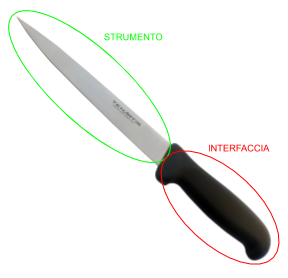
\includegraphics[width=0.7\textwidth]{../immagini/interfaccia.png}
	\caption{L'interfaccia è ciò che consente l'interazione, il controllo e la comunicazione con uno strumento.}
\end{figure}


Quando parliamo di \textbf{User Interface o UI}, in italiano Interfaccia Utente, parliamo quindi dello spazio di un sistema dove avviene l'interazione fra uomo-macchina. Tipicamente, si parla di UI in ambito informatico e tecnologico e quindi le interfacce utente sono comunemente identificate come sistemi atti a mettere in comunicazione l'uomo con computer, sistemi informatici e oggetti intelligenti.

L'obiettivo primario dell'interazione fra uomo e macchina è quello di consentire all'utente di controllare e far funzionare la macchina in modo efficace. L'interfaccia deve quindi essere progettata per semplificare l'interazione fra l'uomo e la macchina rendendo così l'esperienza d'uso piacevole e prolifica. L'interazione fra uomo e macchina deve sempre essere facile, efficiente e divertente così da massimizzare la User Experience del prodotto.

E' importante ricordare che l'uomo si è evoluto grazie alla sua capacità di adattamento che ha la sua massima espressione nel libero arbitrio e nella capacità di prendere decisioni non necessariamente basate sulla logica ma piuttosto sulle sensazioni e intuizioni. Viceversa le macchine hanno un comportamento puramente deterministico e pertanto non hanno nessuna capacità di adattamento. L'interfacci uomo macchina va quindi ad avere un ruolo fondamentale nell'interazione fra le parti dal momento che abilita la comunicazione fra due realtà aventi principi e modalità di "funzionamento" diametralmente opposte.

Un'interfaccia ben progettata consente all'utente di controllare l'apparato richiedendo uno sforzo fisico e cognitivo minimo. La buona interfaccia massimizza inoltre la quantità di informazioni utili trasferite all'utente durante l'interazione evitando un sovraccarico informativo che provocherebbe nell'utente confusione e quindi frustrazione.

\begin{figure}[!h]
	\centering
	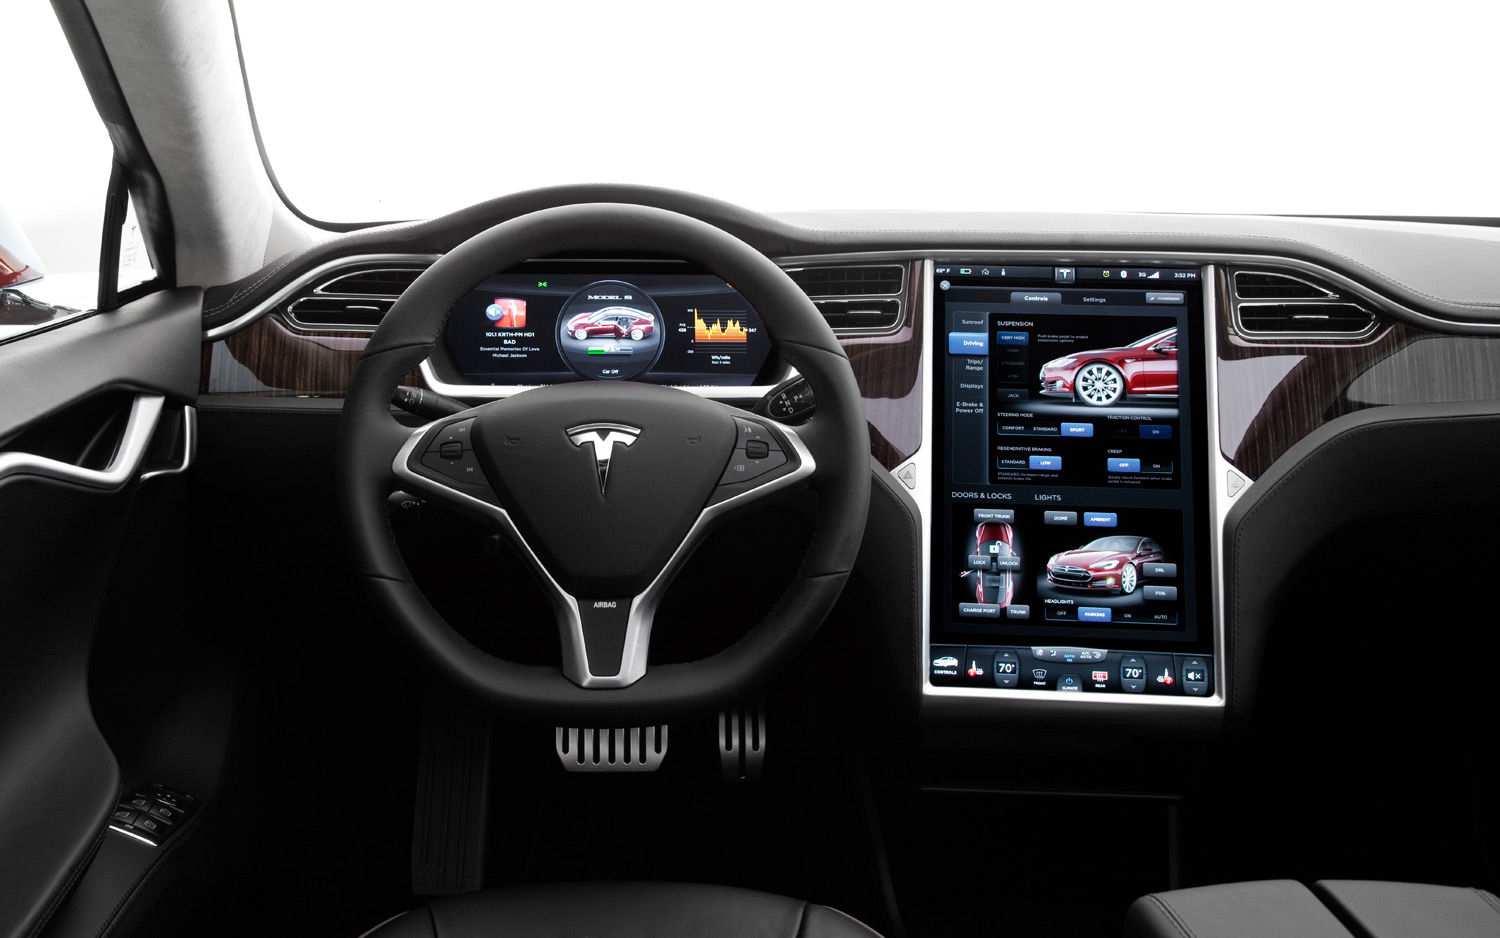
\includegraphics[width=0.9\textwidth]{../immagini/tesla.jpg}
	\caption{Cruscotto della Tesla model S. Fonte: 
https://pinxcars.com/2013-tesla-model-s-cockpit/}
\end{figure}

Per questo motivo, la progettazione di un'interfaccia è per definizione un'attività interdisciplinare che va oltre la programmazione grafica e abbraccia la psicologia, le neuroscienze, il design e la fisica.

Le interfacce sono organizzabili secondo livelli. L' \textbf{HID o Human Interface Device} è la periferica grazie al quale l'utente interagisce con il sistema; come ad esempio mouse, monitor, gamepad, ecc.. Lo \textbf{HMI o Human Machine Interface} è invece un concetto che astrae dall' HID. Con HMI, si intende infatti, tutto il sistema di interazione uomo macchina che usa l'HID come elemento di contatto fisico con l'utente. Nel computer per esempio, la HMI è il sistema mouse+cursore+finestre. Il mouse e il monitor sono HID.

Quando la macchina in questione è un computer, HMI diviene \textbf{HCI o Human Computer Interface}.

\section{Classificazione delle interfacce}
Le interfacce utente sono tipicamente organizzate sulla base dei sensi che utilizzano per stabilire l'interazione fra umano e macchina. Gli umani possiedono cinque sensi (Tatto, Vista, Udito, Olfatto e Gusto). Questo porta ad identificare cinque categorie di interfacce possibili, più una sesta che è legata al cosidetto senso dell'orientamento (balance in inglese) che però non è considerato un senso vero e proprio nella fisiologia umana.

Possiamo quindi organizzare le interfacce in 6 categorie:
\begin{itemize}
	\item \textbf{Tactile UI} (touch, tatto)
	\item \textbf{Visual UI} (sight, vista)
	\item \textbf{Auditory UI} (sound, udito)
	\item \textbf{Olfactory UI} (smell, olfatto)
	\item \textbf{Gustatory UI} (taste, gusto)
	\item \textbf{equilibrial UI} (balance, equilibrio)
\end{itemize}

La maggior parte delle interfacce utente utilizza però più di un senso umano per stabilire il collegamento. Le interfacce che usano più di un senso sono dette \textbf{CUI o Composite User Interface}.
Le più comuni e note CUI sono chiaramente le famose \textbf{GUI o Graphical User Interface}, le quali sono composte da interfacce grafiche (visual) e tattili (tactile). 

Se ad una GUI andiamo ad aggiungere anche il suono otteniamo una \textbf{MUI o Multimedia User Interface}.

Quindi quando ci si riferisce all'interfaccia di una app con il termine GUI spesso compiamo un errore perchè ormai la maggior parte dei dispositivi informatici ha anche una sorgente sonora che è utilizzata durante l'interazione (feedback audio del touch sullo schermo, per esempio) e quindi ci troviamo di fronte ad una MUI e non ad una GUI.


È bene sottolineare che \textbf{estendere le interfacce con più canali (sensi) non è sempre una buona idea
}. Prendiamo ad esempio i video di Facebook, i video vengono riprodotti di default con l'audio disattivato per aumentare l'usabilità del sistema. Gli ingegneri di Facebook si sono accorti infatti che la maggioranza delle persone che visualizzando i video, mutavano immediatamente il suono per varie ragioni (e.g. privacy o utilizzo di Facebook in momenti non opportuni), quindi hanno reso questa opzione di default. Ovviamente se ragionassimo in termini di capacità e possibilità dell'interfaccia sembrerebbe assurdo bloccare di default l'utilizzo di un canale.
Questo processo di anali ha portato poi a far evolvere il mondo dei video online inserendo di default i sottotitoli. Siamo quindi in una situazione in cui per aumentare l'usabilità del sistema se ne riducono le funzionalità (di default).

%Questo, oltre ad essere un ottimo esempio di MUI riprogettata in GUI, è anche un esempio di tecnica ideata per gli utenti disabili e riusata per far fruire il prodotto a quelle personas che lo utilizzano in momenti in cui non possono usufruire dell'audio.

\begin{figure}[!h]
	\centering
	
\includegraphics[width=0.9\textwidth]{../immagini/flora_video.png}
	\caption{I video di Facebook sono in muto di default per aumentare l'usabilità del sistema. Fonte: 
https://www.facebook.com/Lastknight/posts/10158944882367053}
\end{figure}



\section{Categorizzare le CUI}
Le CUI possono essere categorizzare in tre diverse macrocategorie:

\begin{itemize}
	\item \textbf{Standard}: usano dispositivi standard come tastiere, mouse e monitor
	\item \textbf{Virtual}: Bloccano all'utente l'interazione con il mondo reale e creano un mondo virtuale che funge da interfaccia fra l'utente e la macchina.
	\item \textbf{Augmented}: Non bloccano all'utente la percezione del mondo reale ma la vanno ad arricchire. L'interfaccia è quindi un mix di contenuti reali e virtuali che vanno ad arricchire la realtà \textbf{espandendola}.
\end{itemize}

\begin{figure}[!h]
	\centering
	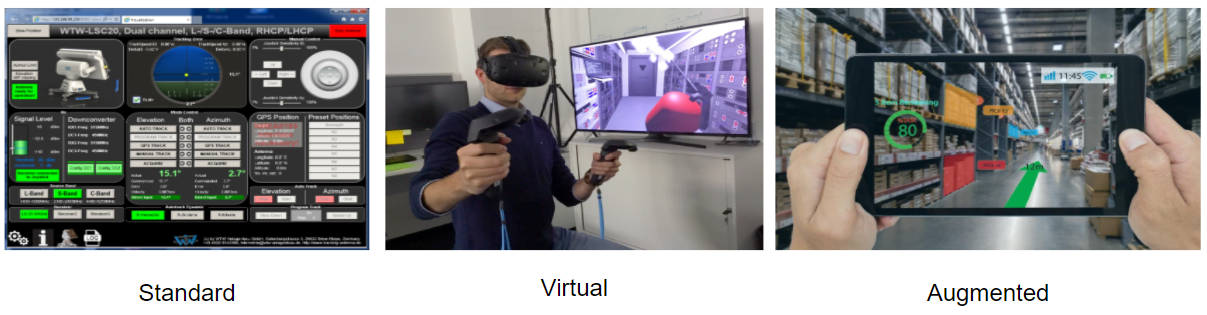
\includegraphics[width=\textwidth]{../immagini/standard-virtual-interfaces.png}
	\caption{Le interfacce possono essere di tipo Standard, Virtuale o Aumentato.}
\end{figure}

Le CUI possono essere anche \textbf{classificate tramite il numero di sensi che utilizzano}. Ad esempio, lo \textit{Smell-O-Vision} è una CUI standard 3S, cioè è una normale interfaccia di tipo standard che nell'utilizzo coinvolge 3 sensi dell'utente (Visione, Udito e Olfatto). Se si aggiungesse un quarto senso (per esempio le poltrone mobili dei cinema 4D) diventerebbe 4S.

Quando un'interfaccia utente interagisce con tutti i sensi umani viene chiamata \textbf{Qualia Interface}. il termine Qualia interface deriva dalla \textbf{teoria filosofica dei Qualia} (https://it.wikipedia.org/wiki/Qualia).

Il Microsoft Reactable è un interessante esempio di interfaccia aumentata 3S (MUI) (Figura \ref{fig:react-table}).

\begin{figure}[!h]
	\centering
	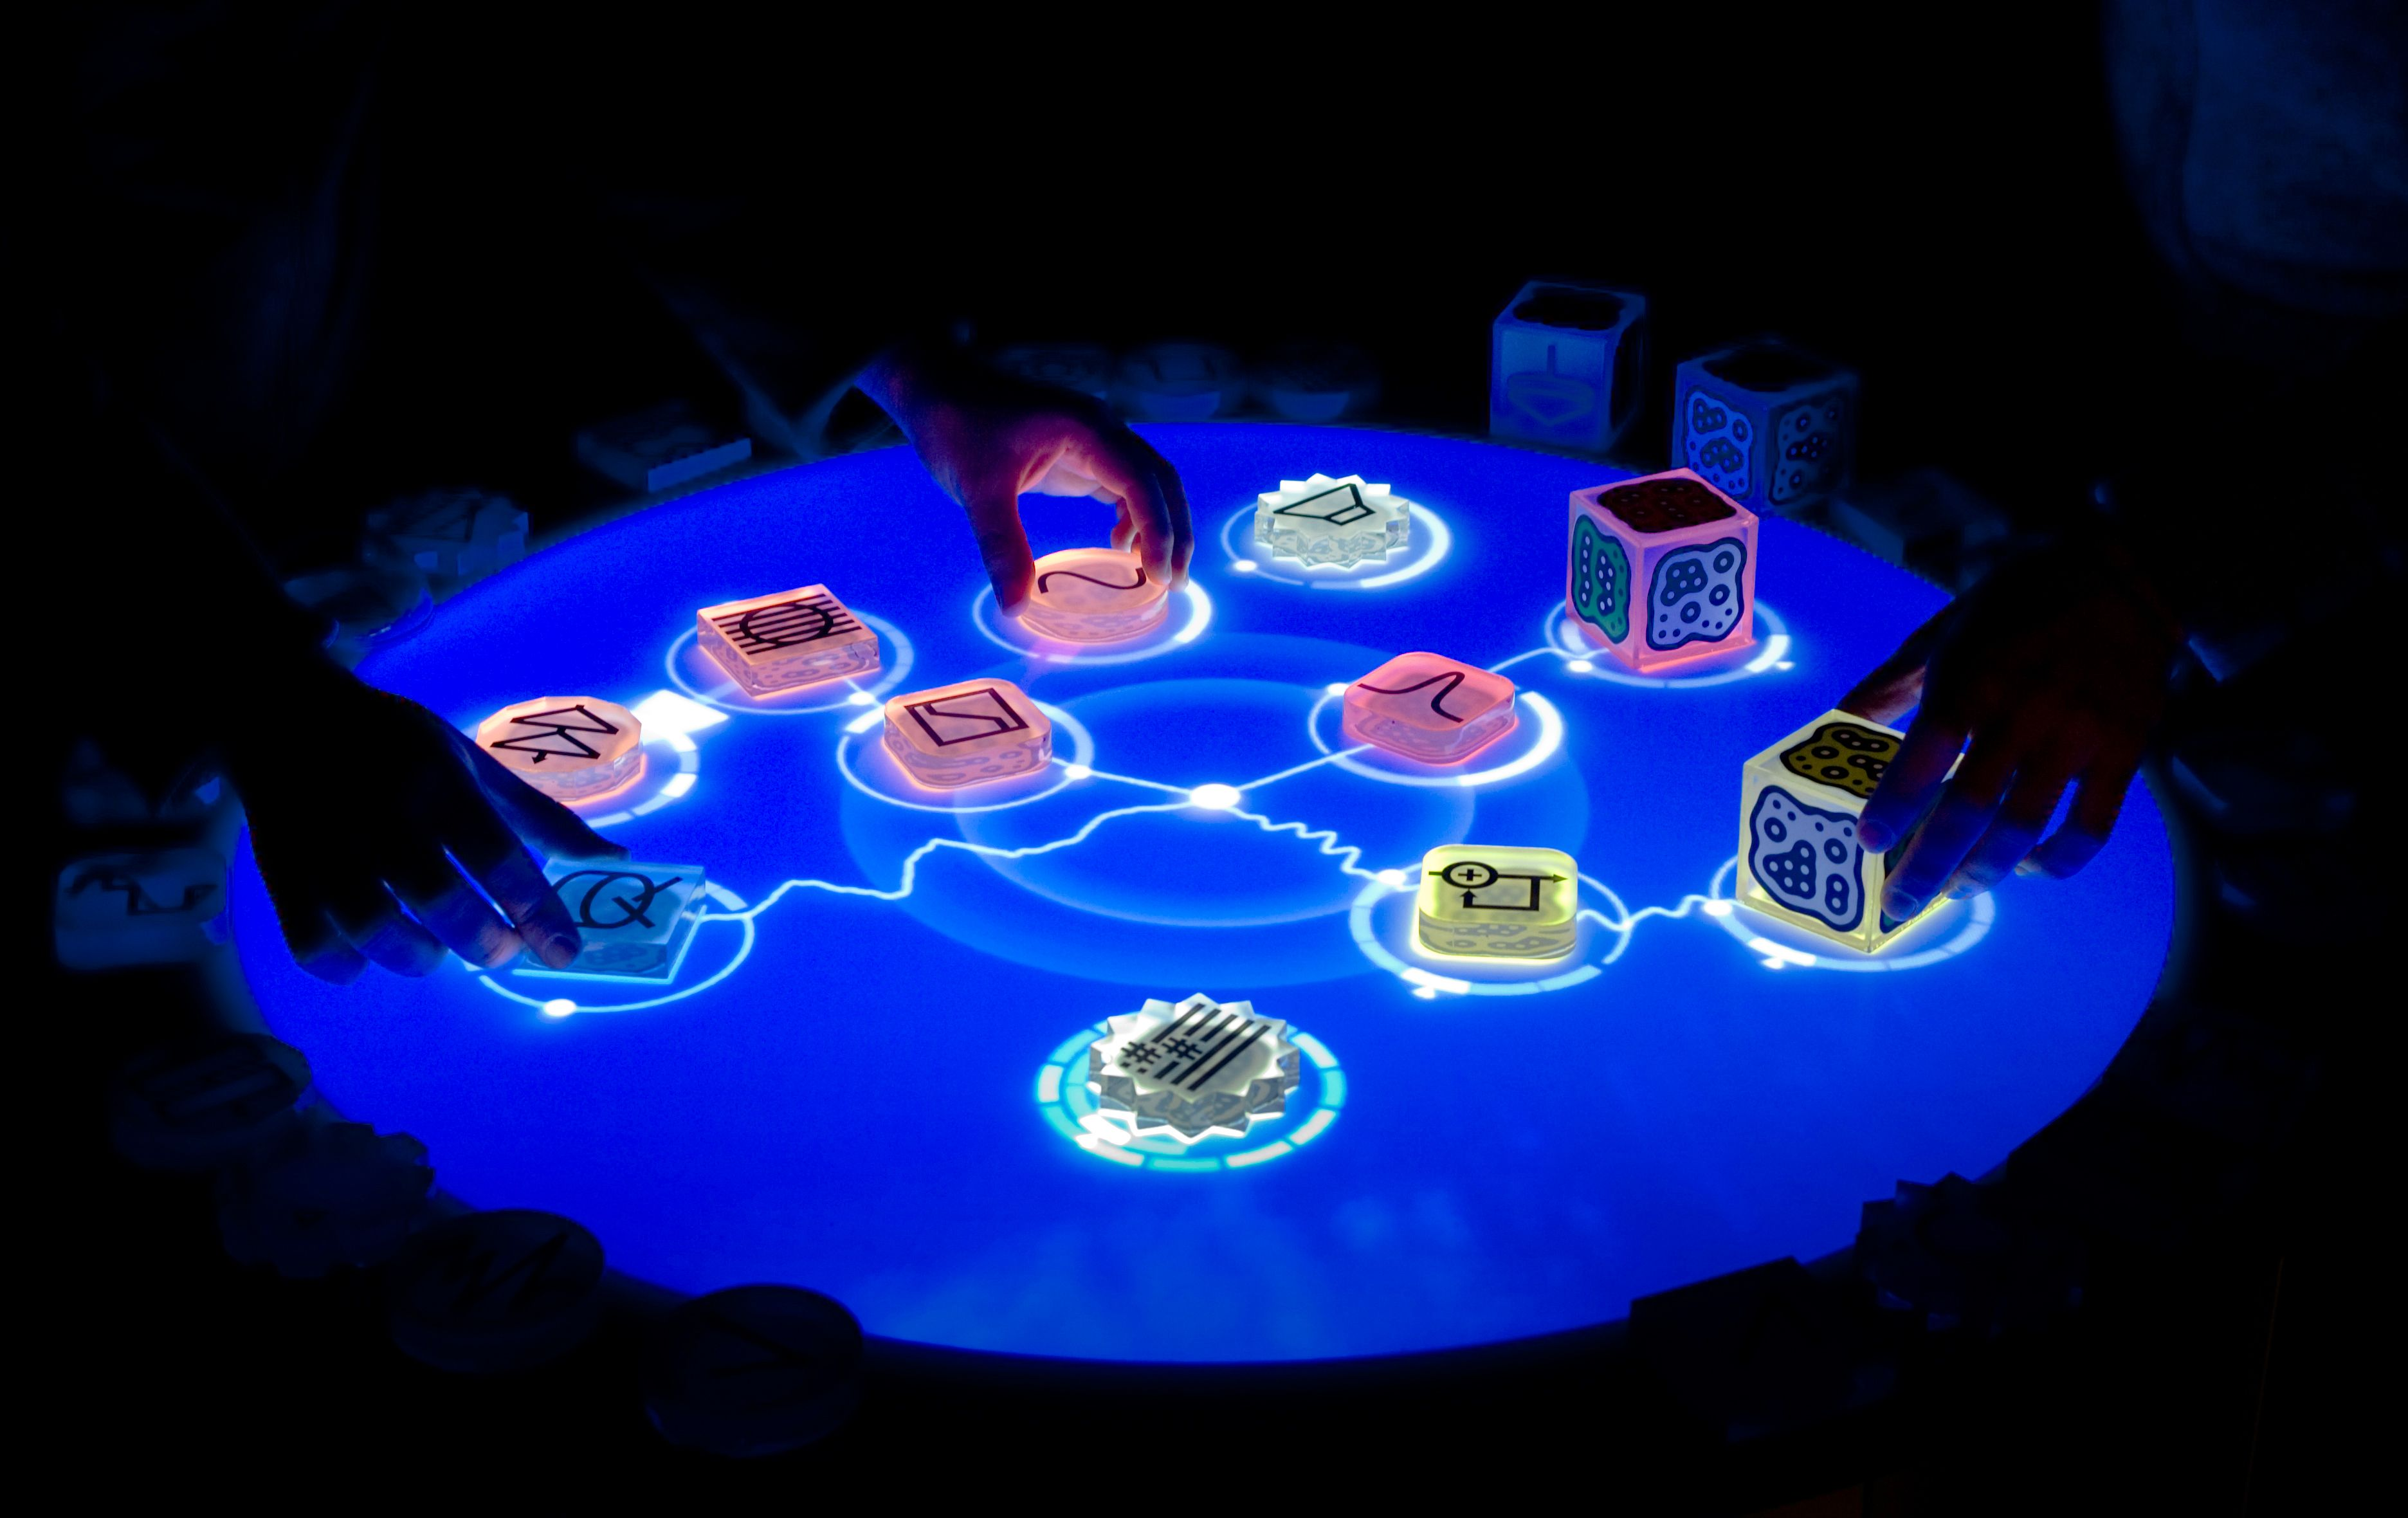
\includegraphics[width=\textwidth]{../immagini/react.jpg}
	\caption{Microsoft Reactable.}
	\label{fig:react-table}
\end{figure}



\pagebreak

 %Le interfacce utente
%\chapter{UX Design}
\begin{flushleft}
	\textit{Quali processi e metodi utilizzare per portare avanti il progetto di un
		prodotto software?}
\end{flushleft}

In questo capitolo si analizzeranno diversi processi.
Essi non vanno identificati come fasi ben definite e statiche, da seguirsi una dietro l'altra, bensì come \textbf{fasi} \textbf{dinamiche} e \textbf{alternabili}.

\section{Personas}
Identificato correttamente il problema mediante la \textbf{Task Analysis}, come si  possono creare elementi individuali? Come si identificano le così dette le \textbf{Personas}?

\begin{figure}[!h]
	\centering
	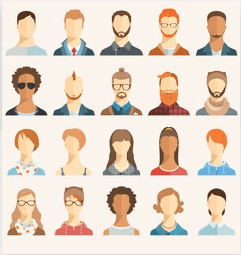
\includegraphics[scale=0.55]{immagini/Personas.png}
\end{figure}

Il primo passo da fare dopo la Task Analysys è \textbf{identificare le personas}.
Una \textbf{personas} è l'\textbf{archetipo di uno dei possibili utenti}. Scrivere e
identificare le personas aiuta a colmare la distanza tra il cliente e l'azienda, in modo da capire cosa vuole e cosa si aspetta l'utente dal prodotto, ma anche cosa gli crea frustrazione nell'usarlo. Esistono molte \textbf{tecniche} atte a fare fare un'analisi degli utenti e che aiutano i progettisti a identificare e a scrivere le personas:

\begin{itemize}
	\item \textbf{Task Analysis}.
	\item \textbf{Feedback} tra i quali: analisi delle attività, interviste e focus groups.
	\item \textbf{Prototipazione}.
\end{itemize}

Sorge spontanea la domanda seguente: \textit{ma quante personas è bene definire}?
Per rispondere a questa domanda ci si basa sul \textbf{Principio di Pareto}: \begin{center}
	\textit{Concentrarsi sul 20\% degli utenti che utilizzerà il prodotto per l'80\% dell'uso complessivo.}
\end{center}

\pagebreak

\section{Requirements}

Un \textbf{requirement} è un servizio o una caratteristica che soddisfa un bisogno di un utente.
I requirements possono essere funzioni, vincoli, regole aziendali o altri tipi di elementi di cui il prodotto deve essere dotato per soddisfare le esigenze degli utenti. È quasi ovvio che trovare i \textbf{requirements corretti} risulta molto più \textbf{semplice} se in precedenza sono state \textbf{individuate} e \textbf{descritte} le \textbf{personas}.

Infatti è controproducente scrivere anticipatamente i requirements,
è complesso se non impossibile descriverli tutti all'inizio di una fase di progettazione. Risulta più facile descrivere i requirements con l'avanzamento del progetto, in modo da poter capire come modificare, eliminare o aggiungere i requirements giusti, tenendo in considerazione anche le personas a cui è destinato il prodotto finale.

Il \textbf{requirements driven development} è un approccio complesso e oneroso e va in \textbf{contrasto} con il metodo \textbf{Agile} che richiede si sia sempre pronti al cambiamento. Questo approccio così poco flessibile sta andando sempre meno di moda tuttavia è bene seguirlo una volta definiti i requirements per quel 20\% di software che utilizzerà l'80\% delle personas.

Esistono \textbf{due tipi di requirements} per il mondo della UI:

\begin{itemize}
	\item \textbf{Funzionali}:
	      descrivono quali funzionalità deve avere il software. Rispondono alla domanda:
	      \textit{Cosa fa?}
	\item \textbf{Non funzionali}: specificano i tratti qualitativi del prodotto. Rispondono alla domanda: \textit{Come lo fa?} e descrivono inoltre
	      attributi come sicurezza affidabilità e manutenibilità.
\end{itemize}

\section{User Stories}
Dopo aver definito \textbf{personas} e \textbf{requirements}, il prossimo passo è la scrittura delle \textbf{User Stories}.

Una \textbf{user story} è una breve descrizione che identifica l'utente insieme al suo
obiettivo e alle sue necessità, determina \textbf{chi è}, \textbf{di cosa ha bisogno e perché ne ha bisogno}. Tipicamente ci sono una o più user stories per ogni personas, ma \textbf{non il contrario}: avere più personas per una user story significa aver descritto la medesima persona con termini differenti e quindi averne introdotta una ridondante.
Se una user story non copre tutte le sfaccettature della singola persona che dovrebbe descrivere è indizio del fatto che tale persona potrebbe essere troppo \textbf{ampia}, ed è bene che venga suddivisa in più personas.

Una user story è un \textbf{requirement} espresso \textbf{dalla prospettiva del cliente}.

Con le user stories si ottengono due importanti risultati: si \textbf{migliorano le descrizioni delle personas}, migliorandone il dettaglio e arricchendole con una narrativa, e si ha un elemento tangibile per valutare lo sviluppo del prodotto e fare il punto della situazione.
Esiste uno schema ben preciso per scrivere una user story:

\begin{center}
	\textbf{\large As a [role], I want [feature] because [reason]}
\end{center}

\begin{flushleft}
	\textit{Chi scrive le user stories?}
\end{flushleft}

\textbf{Tutti}! È responsabilità del proprietario del prodotto assicurarsi che vengano scritte delle stories giuste e corrette, ma non significa che le debba
scrivere lui stesso. Nel corso di un buon progetto Agile ci si aspetta che ogni membro del team partecipi alla scrittura delle user stories secondo un \textbf{metodo collaborativo}.

\pagebreak

\begin{flushleft}
	\textit{A che livello è bene scriverle?}
\end{flushleft}

Uno dei grandi benefici delle user stories è che possono essere
scritte a \textbf{vari livelli di dettaglio}.

Possiamo avere user story di livello \textbf{epic}, ovvero in grado di
coprire un grande quantità di funzionalità, tipicamente sono disutili ma possono diventare interessanti se spacchettate in user stories più piccole e, di conseguenza, più dettagliate. Una \textbf{user story epic} può essere \textbf{divisa} in decine o centinaia di user stories più piccole.

I dettagli possono essere aggiunti sostanzialmente in due modi:
\begin{enumerate}
	\item Suddividendo una user story in user stories più piccole e quindi più dettagliate.
	\item Aggiungendo \textbf{condizioni di soddisfacimento dell'utente}, ovvero  dettagli che contribuiscono al grado di soddisfacimento dell'utilizzatore del prodotto, suddividendole per ogni eventuale membro di soddisfacimento. Quest'ultima è una tecnica molto difficile da utilizzare nel mondo della progettazione software.
\end{enumerate}

\section{Scenarios}

Gli \textbf{scenarios} sono l'\textbf{evoluzione delle user stories}. Una user story sintetizza in brevi frasi cosa fa l'utente con il software e quale bisogno deve soddisfare.

Lo \textbf{scenario estende la user story} andando a descrivere anche quali motivazioni hanno portato l'utente ad usare il software e come egli si comporterà nel suo utilizzo. Inoltre gli scopi o \textbf{goals} delle personas vengono \textbf{estesi} e descritti in maniera più ampia.

\begin{flushleft}
	\textit{Ma a cosa serve uno scenario?}
\end{flushleft}

Le \textbf{user stories} sono \textbf{sintetiche}, \textbf{brevi}, dicono cosa sviluppare e poco più, sono informative e comprensibili \textbf{solo} agli \textbf{addetti al mestiere}. Gli \textbf{scenarios}, essendo più ricchi in dettaglio, sono più comprensibili agli \textbf{stakeholders}, quindi sono \textbf{utili per comunicare e interloquire con persone fuori dal team di sviluppo}. Servono soprattutto per allinearsi con le richieste del cliente ma sono  utili anche all'interno del team per allineare le idee.

Un buon scenario risponde alle \textbf{seguenti domande chiave}:

\begin{itemize}
	\item \textbf{Chi è l'utente?}
	\item \textbf{Quale è la motivazione che lo ha spinto ad usare il prodotto e cosa si aspetta da esso?}
	\item \textbf{Qual è il suo obbiettivo?}
\end{itemize}

In alcuni casi uno scenario potrebbe includere anche aspetti circa \textit{come} fare le cose, ma ciò appartiene al mondo degli \textit{use cases} che verranno analizzati successivamente.
Per \textbf{definire gli scenarios}, è necessario \textbf{mapparli}. Bisogna partire \textbf{avendo già definito le personas e le relative user stories}, e individuare per ogni persona un \textbf{key task} che essa deve svolgere. Si possono scrivere gli scenarios racchiudendo una o più
user stories relative alla persona ma tipicamente per ogni persona si descrive  almeno uno scenario. È necessario \textbf{focalizzarsi sul key task} e quindi contestualizzare nel miglior modo possibile il goal dell'utente e come è influenzato dal contesto in cui egli si trova.

Quindi grazie agli scenarios \textbf{possiamo determinare}:

\begin{itemize}
	\item I \textbf{punti più importanti} su cui concentrarsi durante il \textbf{processo di progettazione per l'UX}.
	\item Quali fasi del processo richiedono \textbf{ulteriore revisione e attenzione}.
	\item Le \textbf{principali esigenze e motivazioni dell'utente}.
\end{itemize}

\pagebreak

Ci sono \textbf{tre metodi principali per scrivere gli scenarios}:

\begin{itemize}
	\item Piccoli \textbf{goal or task oriented scenarios}: sono brevi, quasi una semplice estensione della dialettica di una user story.
	\item \textbf{Elaborated Scenarios}: sono versione più elaborata e con molto più contesto.
	\item \textbf{Full Scale Task Scenarios}: sono talmente dettagliati che i singoli task delle attività sono praticamente scritti sotto forma di paragrafo. Sono da evitare poiché si rischia gli scenarios così ottenuti siano uguali agli use cases.
\end{itemize}

\section{Use Cases}

Gli use cases sono la naturale evoluzione degli scenarios.
\textbf{Consistono della completa narrativa di quali azioni l'utente compie per svolgere uno scenario}.

Ogni \textbf{caso d'uso} è una \textbf{serie di step monolitici}, è quindi una nuova task list prodotta dal processo di design per ampliare ulteriormente un concetto analizzato e descritto in precedenza mediante la task analysis.
Uno \textbf{scenario} si concentra su una situazione che coinvolge uno o più \textbf{attori}, mentre un
\textbf{caso d'uso} è incentrato su una \textbf{persona}, come essa si comporta, che decisioni prende e come interagisce con la nostra piattaforma o software. I casi d'uso aggiungono informazione perché aiutano a \textbf{spiegare come dovrebbero comportarsi
	il sistema e il processo}, inoltre aiutano anche nella fase progettuale di brainstorming e danno un'idea su cosa potrebbe andare storto. Forniscono inoltre un elenco di obiettivi che può essere utilizzato per stabilire e valutare la complessità del sistema. I casi d'uso sono \textbf{diretti allo sviluppo}.

Con dei \textbf{casi d'uso ben fatti} si può passare direttamente all'\textbf{implementazione} poiché \textbf{delimitano precisamente cosa deve fare il sistema e come si deve comportare nelle varie situazioni}.

In un caso d'uso sono \textbf{inclusi}:

\begin{multicols}{2}
	\begin{itemize}
		\item \textbf{L'utente}.
		\item \textbf{Cosa vuole fare}.
		\item \textbf{Qual è il suo scopo o goal}.
		\item Gli \textbf{step necessari} per arrivare allo scopo.
		\item I \textbf{feedback} che il sistema restituisce durante i vari step.
	\end{itemize}
\end{multicols}

\textbf{Non sono inclusi} in un caso d'uso:

\begin{multicols}{2}
	\begin{itemize}
		\item Qualsiasi \textbf{dettaglio implementativo o di scelta tecnologica} che non sia un constraint o un requirement.
		\item \textbf{Dettagli} riguardanti l'interfaccia utente.
	\end{itemize}
\end{multicols}

I passaggi da seguire per scrivere un caso d'uso sono:

\begin{multicols}{2}


	\begin{enumerate}
		\item Identificare le \textbf{personas}.
		\item Sceglierne \textbf{una per caso d'uso}.
		\item Identificare i suoi \textbf{obiettivi}.
		\item Discernere i \textbf{task principali} da quelli \textbf{secondari}: applicare il principio di Pareto, quindi focalizzarsi sul basic path e non su casi particolari.
		\item Considerare le sequenze alternative.
		\item Cercare i punti in comune tra i vari casi d'uso e \textbf{accorparli}, riducendoli ove possibile.
		\item Ripetere il procedimento per tutti gli utenti.
	\end{enumerate}
\end{multicols}

Questi passaggi, eseguiti correttamente, consentono di identificare informazioni chiave sugli utenti, utili a costruire prodotti che soddisferanno tutte le possibili personas. \textbf{Ogni passo che ci avvicina all'utente è un passo verso la giusta direzione}.

\pagebreak

%\chapter{Errore Umano}

La maggior parte degli incidenti industriali è causata da errore umano:
le stime si aggirano tra il 75\% e il 95\% del totale.

\begin{flushleft}
	\textit{Come è possibile che tante persone siano così incompetenti?}
\end{flushleft}

La risposta è semplice! Non lo sono, il problema è nella mal progettazione e nel cattivo design.

Si continuano a produrre dispositivi e software che richiedono, a chi li usa, di mantenere per ore un'attenzione ed una vigilanza complete, oppure di memorizzare procedure arcaiche, confuse e usate di rado, magari anche una sola volta nella vita. Si costringono le persone a stare in un ambiente monotono senza nulla da fare per ore e ore, salvo dovere improvvisamente rispondere con rapidità e precisione. Le si sottopone ad un ambiente di lavoro complesso e sovraccarico, dove sono continuamente interrotte durante l'esecuzione di compiti simultanei. L'\textbf{interruzione è una delle cause che più frequentemente portano all'errore umano}.

Uno dei più grandi \textbf{problemi} è l'\textbf{atteggiamento delle persone verso gli errori} commessi. Quando un errore causa perdite economiche o, peggio ancora, danni alle persone, si istituisce una speciale commissione d'inchiesta, che quasi immancabilmente trova i colpevoli.

Il passo successivo è punirli con multe, il licenziamento o addirittura il carcere. Essi vengono incolpati
e puniti o, nella migliore delle ipotesi, incolpati e riaddestrati. Tutto questo però non
risolve il problema: lo \textbf{stesso errore continuerà a presentarsi}.  Per evitare di incorrere nuovamente nell'errore, quando esso viene commesso, è bene  studiarne le cause, per poi ridisegnare il prodotto o le procedure in modo che esso non si ripeta o, se dovesse ripetersi, che i danni siano ridotti al minimo.

\section{Root Cause Analysis}
La \textbf{Root Cause Analysis} consiste nell'indagare l'incidente finché non si trova la singola causa che ne è l'origine. Ovvero il momento nel tempo quando effettivamente qualcuno ha preso decisioni o eseguito azioni sbagliate e,
una volta fatto ciò, accertare da cosa è derivato lo sbaglio. Purtroppo, troppo spesso, il processo si ferma non appena si scopre che una persona ha agito in maniera impropria, additandola come \textit{colpevole}.

Cercare di trovare la causa di un incidente suona bene, ma ha due difetti.

\begin{enumerate}
	\item La maggior parte degli incidenti \textbf{non ha una sola causa}. Da qui il \textbf{modello a groviera degli incidenti} di James Reason.
	\item Solitamente l'analisi delle cause profonde si ferma non appena trovato un errore umano.
\end{enumerate}

\pagebreak

\begin{figure}[!h]
	\centering
	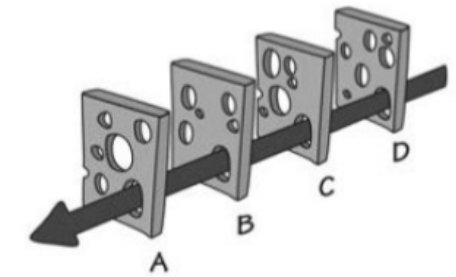
\includegraphics[scale=0.55]{immagini/Groviera.png}
	\caption{Modello a groviera.}
\end{figure}

Se una macchina smette di funzionare per un guasto o un malfunzionamento
si cerca di capire come mai si è rotta o cosa l'ha portata a guastarsi. È
opportuno fare lo stesso quando si scopre un errore umano: \textbf{individuarne le cause}.

Quando durante l'analisi delle cause profonde si incontra, nella concatenazione di cause ed effetti, un errore umano, \textbf{il lavoro è appena cominciato}: bisogna capire \textbf{perché} l'errore \textbf{è accaduto e cosa si può fare per prevenirlo}.

\section{I cinque perché}

L'analisi delle cause profonde mira a determinare la causa \textbf{prima di un evento}, non la causa immediata.

In Giappone da tempo si usa a questo scopo una procedura detta \textit{``dei \textbf{cinque perché}''} ideata da Sakichi Toyoda e impiegata dalla Toyota nell'ambito del sistema di controllo qualità dei suoi prodotti.

Fondamentalmente quindi quando si cerca la ragione di un evento non ci si deve fermare dopo averne trovata solo una, ma bisogna continuare ad indagare fino a che non si trovano le \textbf{vere cause di fondo}.

Va ripetuta davvero cinque volte?

No, ma chiamarla \textit{procedura dei cinque perché} sottolinea la necessità di proseguire anche dopo aver trovano una causa apparente.

Vediamo un esempio: \textbf{il veicolo non si accende}.

\begin{enumerate}
	\item \textbf{Perché?} La batteria è morta.
	\item \textbf{Perché?} L'alimentatore non funziona.
	\item \textbf{Perché?} La cinghia dell'alternatore non funziona.
	\item \textbf{Perché?} La cinghia dell'alternatore era ben oltre il suo tempo di servizio e non è stata sostituita.
	\item \textbf{Perché?} Il veicolo non è stato mantenuto secondo le tempistiche raccomandate.
\end{enumerate}

Quando le persone sbagliano, bisogna \textbf{cambiare il sistema} in modo da evitare l'errore
e, se non è possibile eliminarlo del tutto, almeno fare in modo di ridurne gli effetti.

Se il sistema lascia sbagliare gli utenti è \textbf{mal progettato}, se il sistema induce all'errore, allora è \textbf{progettato malissimo}.

\pagebreak

\begin{flushleft}
	\textit{Perché le persone sbagliano?}
\end{flushleft}

Perché il design si concentra sulle esigenze del sistema
e delle macchine, non su quelle degli utenti. Le macchine hanno bisogno in genere di
comandi precisi, obbligando l'operatore a introdurre esatte informazioni numeriche. Gli esseri umani non sono adatti ad esercitare grande precisione e commettono spesso
errori quando devono digitare lunghe sequenze di numeri o lettere.

Gli umani sono creativi, curiosi, costruttivi, particolarmente bravi nel creare modi nuovi di fare le cose e nel cogliere nuove opportunità. Compiti monotoni, ripetitivi e precisi contraddicono tali qualità e vi entrano in conflitto.

\section{Definizione di errore}
Si definisce \textbf{errore umano} ogni deviazione dal comportamento \textit{appropriato}. Il termine ``appropriato'' è da prendere con le pinze, perché in molte circostanze si scopre quale fosse il comportamento giusto solo successivamente.

Generalmente comunque si chiama \textit{errore} ogni comportamento che si discosta da quello generalmente accettato come giusto o adeguato. \textbf{Errore} è il termine generale per tutte le situazioni sbagliate. È possibile dividere gli errori in \textbf{due} classi:

\begin{multicols}{2}
	\centering
	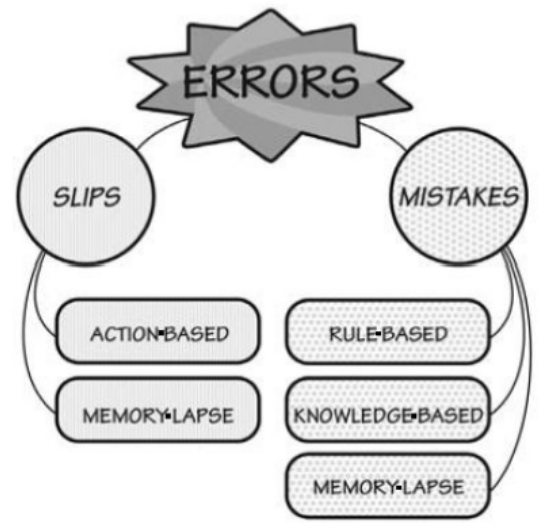
\includegraphics[scale=0.25]{immagini/Errors.png}
	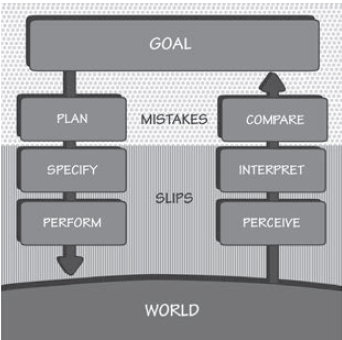
\includegraphics[scale=0.4]{immagini/Errors1.png}
\end{multicols}

\begin{enumerate}
	\item \textbf{Lapsus o Slips}: si ha un lapsus quando s'intende eseguire un'azione e si finisce per eseguirne un'altra. Nel caso del lapsus, l'azione eseguita non è quella voluta. Ci sono \textbf{due tipi principali di lapsus}:
	      \textbf{lapsus di azione e lapsus di memoria}.
	      Nel primo caso si esegue un'azione sbagliata, nel secondo si dimentica di eseguire
	      l'azione o di valutarne i risultati.
	      Esempio di \textbf{lapsus di azione}: versare il latte nel caffè e poi riporre la tazza in frigorifero. L'azione è giusta ma è applicata all'oggetto sbagliato.
	      Esempio di \textbf{lapsus di memoria}: dimenticare di spegnere il fornello dopo aver terminato la cottura. \textbf{I lapsus si hanno nelle fasi attuative e percettive dell'azione.}
	\item \textbf{Errori cognitivi o Mistakes}: si ha un errore cognitivo quando è sbagliato il goal o lo scopo: da quel momento in poi le azioni, anche se eseguite a puntino, fanno parte dell'errore essendo di per sé inappropriate, in quanto parte di un progetto sbagliato. In questo tipo di errore l'azione è corretta ma l'intenzione no.
	      Gli errori cognitivi si suddividono in: \textbf{regola sbagliata}, \textbf{conoscenza sbagliata e dimenticanza}. In un errore generato dall'applicazione della \textbf{regola sbagliata}, la
	      diagnosi della situazione è giusta, ma poi viene scelto un corso d'azione sbagliato,
	      seguendo una regola operativa errata. In un errore causato da \textbf{conoscenza erronea}
	      o \textbf{incompleta}, ad essere sbagliata è la diagnosi stessa della situazione. Gli errori per \textbf{dimenticanza} si hanno invece quando ci si dimentica di qualche passaggio al momento di fissare gli obiettivi, di eseguire una procedura o di valutarne i risultati. \textbf{Gli errori si fanno nelle fasi di tipo cognitivo.}
\end{enumerate}

\pagebreak

\section{Prevenzione dell'errore}

\begin{flushleft}
	\textit{Non dovrebbe essere possibile che un semplice errore provochi un danno diffuso.}
\end{flushleft}

Ecco che cosa dovrebbe essere fatto in fase di prevenzione:

\begin{itemize}
	\item \textbf{Comprendere le cause dell'errore} per minimizzarne il ripresentarsi.
	\item Effettuare \textbf{controlli di sensibilità}, ovvero, chiedersi se le azioni superano il \textit{test del buon senso}.
	\item Rendere possibile \textbf{annullare le azioni} (undo) o rendere più difficile fare ciò che non può essere annullato (per esempio con uso di locks).
	\item \textbf{Rendere} più \textbf{semplice la scoperta e la comprensione degli errori} e semplificarne la risoluzione.
	\item Non trattare l'azione come errore, piuttosto \textbf{aiutare l'utente a compiere correttamente l'azione}.
\end{itemize}

I \textbf{novizi}, gli utenti base, coloro meno esperti del sistema cadono in \textbf{errori per lo più cognitivi} poiché non hanno una base di conoscenza adeguata e sufficientemente strutturata, viceversa, gli \textbf{utenti esperti} che usano il software o il sistema tutti i giorni e che lo conoscono bene commettono più errori di tipo \textbf{lapsus} poiché tendono ad eseguire i compiti in maniera automatica, quasi istintiva, affidandosi al controllo subconscio, mentre un
principiante è costretto a fare molta attenzione, cosicché incorre meno nei lapsus.

Gli \textbf{errori cognitivi} nascono dalla scelta di scopi e piani d'azione inadeguati, oppure, in sede di valutazione, dal confronto errato tra risultati e scopi. In altre parole dipendono da \textbf{informazioni ambigue o poco chiare sullo stato attuale del sistema e dalla mancanza di un buon modello concettuale}.

Si esamineranno adesso quali possono essere le cause di errore e come è possibile prevenirle.

Le \textbf{interruzioni} sono una delle più grandi cause di errore, \textbf{soprattutto i lapsus}. Quando un'attività viene interrotta da qualche evento, il costo in attenzione è molto maggiore della perdita di tempo causata dell'interruzione. Per riprendere il lavoro è necessario ricordare precisamente il precedente stato dell'attività: quale era l'obiettivo, a che punto del ciclo dell'azione si era rimasti e quale era lo stato del sistema.

La maggior parte dei sistemi rende difficile la ripresa di un azione a seguito di un'interruzione. Tuttavia riducendo i passaggi dell'azione è possibile diminuire il costo d'attenzione necessario per riprendere la concentrazione dopo esser stati interrotti.

Un'altra causa di errore sono i \textbf{feedback errati}: avvisi fastidiosi o non necessari che si presentano spesso durante l'uso di un sistema. Spesso vengono silenziati, disattivati o ignorati, \textbf{facendo perdere di significato anche quelli utili per il raggiungimento dello scopo}.

Se si usano i feedback per segnalare errori ed essi sono stati disattivati dall'utente, egli cadrà in errore non conoscendone nemmeno il motivo. \textbf{Avvisi e metodi di sicurezza vanno usati con cura e intelligenza}.

Un numero sempre maggiore di macchine e sistemi offrono informazioni attraverso l'uso di interfacce vocali , ma come tutti gli approcci anche questo ha dei pro e
dei contro. Da una parte consente di fornire informazioni precise, specialmente quando
l'attenzione visiva è diretta da qualche altra parte, ma se l'ambiente è rumoroso o se ci sono diversi avvisi vocali contemporaneamente, tali avvisi possono non essere compresi o risultare addirittura fastidiosi.

\pagebreak

\begin{figure}[!h]
	\centering
	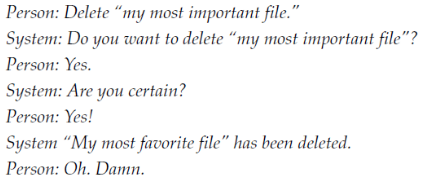
\includegraphics[scale=0.6]{immagini/Damn.png}
\end{figure}

Per prevenire errori è possibile quindi utilizzare:
\begin{itemize}
	\item \textbf{Constraints}: aggiungendo vincoli alle azioni. I sistemi elettronici hanno un'ampia selezione di metodi che possono essere usati per ridurre l'errore. Uno di questi può essere \textbf{segregare i controlli}, cosicché controlli confondibili tra loro vengano piazzati lontani l'uno dall'altro. Un altro è di \textbf{separare i moduli}, cosicché qualsiasi controllo non direttamente rilevante all'operazione corrente non sia visibile a schermo ma richieda uno sforzo extra per essere raggiunto.
	\item \textbf{Undo}: comando che annulla le operazioni effettuate dal precedente. I sistemi migliori hanno \textbf{più livelli di undoing} in modo tale da annullare intere sequenze di azioni.
	\item \textbf{Messaggi d'errore e di conferma}: molti sistemi cercano di prevenire l'errore chiedendo conferma prima di eseguire un comando, specialmente quando l'azione distruggerà qualcosa di importante. Tuttavia queste richieste sono spesso mal temporeggiate, perché \textbf{dopo aver richiesto un'operazione le persone sono solitamente certe di volerla compiere}. Un controllo migliore sarebbe visualizzare sia l'azione da compiere che l'oggetto interessato, con l'opzione annulla o prosegui.\textbf{ I messaggi di avviso sono sorprendentemente inefficaci contro gli errori}.

	\item  \textbf{Controlli di Sensibilità}: i sistemi elettronici presentano il vantaggio di poter controllare che l'operazione richiesta sia \textbf{sensibile} o \textbf{ragionevole}. Ad esempio verificare che l'importo indicato sia giusto, magari esponendo un avviso in caso di numeri eccessivamente grandi.
\end{itemize}

In estrema sintesi e ricollegandosi all'esempio della groviera, per ridurre gli errori si hanno le seguenti possibilità:

\begin{figure}[!h]
	\centering
	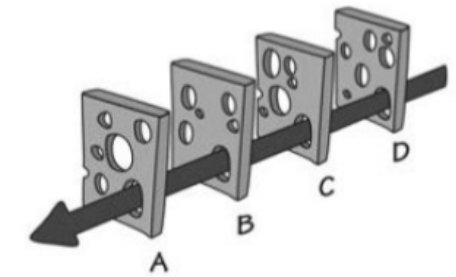
\includegraphics[scale=0.5]{immagini/Groviera.png}
\end{figure}

\begin{itemize}
	\item \textbf{Aumentare il numero di controlli} (le fette).
	\item \textbf{Migliorare il modello concettuale dell'utente}. (ridurre il numero di buchi, o rendere più piccoli i buchi esistenti, magari con un modello concettuale minimale e dei constraints)
	\item \textbf{Allertare l'operatore umano quando diversi buchi si allineano}.
\end{itemize}

\pagebreak



\pagebreak

%\chapter{UX e UI di prodotti interconnessi}

Quando ci si trova di fronte al compito di progettare l'interfaccia di un \textbf{dispositivo
	connesso}, si tende si tende ad adottare un approccio in linea alla \textit{vecchia
	scuola} della UI e UX. Si tende quindi a dare maggior peso e a spendere maggior concentrazione su aspetti come l'estetica delle interfacce e la forma del prodotto fisico. \textbf{Per l'IoT ciò non basta}.

Un prodotto interconnesso può avere un'ottima UI ma una pessima UX, esso non è costituito solamente dalla sua apparenza o dalla sua interfaccia, ma è \textbf{l'insieme delle due cose}.

Internet è un \textbf{mezzo di comunicazione}, fatto dagli uomini per gli uomini, \textbf{l'Internet of Things o IoT è un sistema di dispositivi informatici interconnessi}, macchine meccaniche o digitali \textbf{fornite di un identificatore unico detto UID}.

Esse possiedono la capacità di trasferire i dati sulla rete senza richiedere l'interazione uomo-uomo o uomo-computer.
La differenza tra i due mondi è sottile e spesso gli oggetti IoT sono creati per comunicare perfettamente tra di loro, ma hanno una pessima UI per l'uso umano, e
di conseguenza sono portatori di una pessima UX.

\section{Industry 4.0}

Il termine \textbf{Industria 4.0} indica l'ultima fase del processo con cui l'automazione industriale \textbf{integra} nuove \textbf{tecnologie produttive} per \textbf{migliorare} le condizioni di lavoro, creare nuovi modelli di business e aumentare la produttività e la qualità produttiva degli impianti.

I sistemi computerizzati monitorano i processi fisici, creando copie virtuali del mondo su cui sono basate le scelte e le decisioni future per il business dell'azienda.

\begin{figure}[!h]
	\centering
	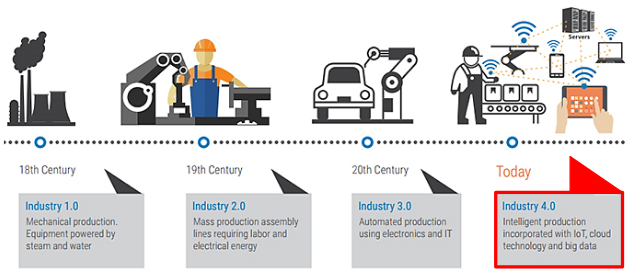
\includegraphics[scale=0.7]{immagini/Industry4.png}
\end{figure}

\pagebreak

Il problema di ogni tappa della rivoluzione industriale risiede nell'aumento esponenziale della \textbf{complessità informatica}. I dati parlano chiaro: il salto informativo dall'industria 3.0 all'industria 4.0 è pari al totale del salto effettuato da quando si usava l'asino come mezzo di locomozione fino alle attuali tecnologie.

\begin{figure}[!h]
	\centering
	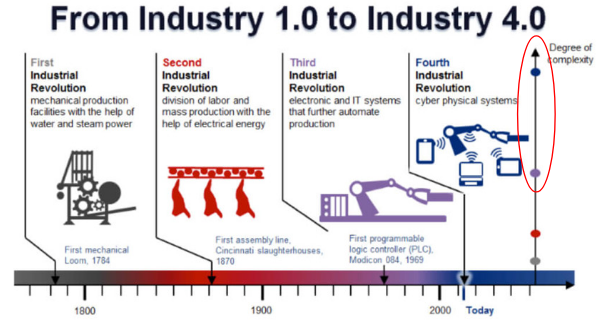
\includegraphics[scale=0.6]{immagini/Revolution.png}
\end{figure}

Quello che prima era un \textbf{processo produttivo}, con l'industria 4.0 diventa un \textbf{servizio} e la quantità di informazione necessaria cresce incredibilmente, di conseguenza progettare per la UX diventa estremamente complesso.

Ma come mai è importante questa evoluzione? Per le seguenti ragioni:

\begin{itemize}
	\item  Ottimizzando la produzione i profitti aumentano.
	\item Sarà possibile creare \textbf{nuovi modelli di business}.
	\item Saranno accessibili \textbf{nuove tecnologie}.
	\item Sarà possibile trasformare la forza lavoro: da operai in tecnici, capaci di estrarre informazioni dalle macchine e modificare la produzione di conseguenza.
\end{itemize}

Il cuore di un sistema interconnesso, sia di tipo consumer che industriale, è il
\textbf{Digital Twin}. Il \textbf{Digital Twin} è  \textbf{una copia digitale di un bene, di una macchina o di un processo reale esistente}. La comunicazione tra l'oggetto fisico e il Digital Twin è \textbf{continua e bidirezionale}. Tale strumento può essere usato sia per logging che per controllo remoto, ma sopratutto, è utile per simulazioni e manutenzione.

\begin{figure}[!h]
	\centering
	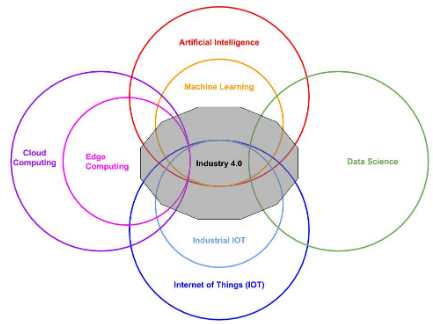
\includegraphics[scale=0.55]{immagini/Holistic.png}
\end{figure}

\pagebreak


\section{Products and Services in the 4.0 era}

\begin{figure}[!h]
	\centering
	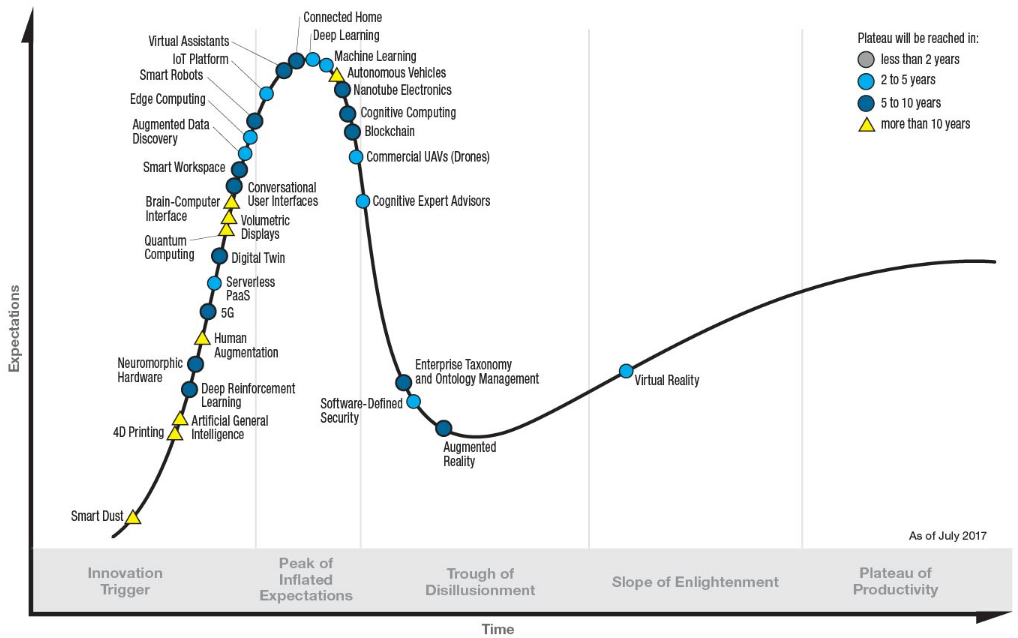
\includegraphics[scale=0.45]{immagini/Hype.png}
	\caption{Gartner Hype Cycle for emerging technologies.}
\end{figure}

L'IoT è solo una tecnologia abilitante, quindi non bisogna progettare per l'IoT bensì bisogna progettare sistemi interconnessi. Ciò altera il paradigma di progettazione: prima erano i computer ad essere dei centri di aggregazione tecnologica: qualche anno fa, ad esempio, in una qualsiasi casa, l'unico oggetto definibile smart era un \textbf{computer}, adesso si hanno più dispositivi connessi per svolgere svariate attività.

Sta sempre più emergendo il concetto di \textbf{intelligenza distribuita} accompagnata da un'\textbf{interfaccia personale}.

I dispositivi che si vuol progettare dovrebbero avere funzionalità altamente \textbf{specifiche} ma veicolate attraverso interfacce \textbf{generiche}. Le interfacce specifiche sono da evitare.

Si prenda, per esempio, un robot da cucina che riesce a fare
di tutto: frullare, centrifugare e cuocere, più una vasta gamma di funzionalità selezionabili, tramite pulsanti, uno per ogni funzione, attraverso un'interfaccia posta sul robot stesso. \textbf{Ciò è da ripudiare} in favore di un robot senza un singolo tasto che capisce da sè cosa va fatto e come farlo.

La progettazione per l'IoT è intrinsecamente più \textbf{complessa} della progettazione di servizi Web. Il design fisico, il design della UX e l'interconnettività di un unico sistema \textbf{non} possono essere gestiti separatamente.

I prodotti connessi pongono i progettisti dinanzi a sfide progettuali nuove, molte delle quali derivano da:

\begin{itemize}
	\item La \textbf{natura} specializzata dei servizi \textbf{IoT}.
	\item La capacità dei dispositivi IoT di fare da \textbf{ponte tra il mondo digitale e fisico}.
	\item Il fatto che molti prodotti IoT siano \textbf{sistemi distribuiti composti da più dispositivi}.
	\item \textbf{Le stranezze del networking}.
\end{itemize}

\pagebreak

\section{Real world context}
Le interfacce, nel mondo dell'IoT, sono sensori e attuatori. I \textbf{sensori} convertono una variabile \textbf{fisica} in un segnale \textbf{elettrico}, mentre gli
attuatori convertono un segnale\textbf{ elettrico} in una variabile \textbf{fisica}.

Gli attuatori possono essere controllati a distanza o automatizzati, ma a differenza dei comandi digitali, le azioni sul mondo reale \textbf{non possono essere annullate}.
Questo contesto fisico di utilizzo crea ulteriori sfide. Nell'IoT non si può dare per
scontato lo stato d'animo dell'utente mentre interagisce con l'oggetto.

Gli oggetti ubiquitari, andando a posizionarsi nei vari angoli della casa o dell'ufficio, si trovano ad interagire con persone che potrebbero momentaneamente \textbf{non essere predisposte all'interazione con un oggetto digitale}, ciò rende l'errore molto più frequente.

Si devono creare quindi oggetti molto semplici sia da capire che da utilizzare.

Un altro aspetto importante è l'\textbf{interusabilità}, cioè la proprietà del sistema di essere usato attraverso \textbf{tutti} i dispositivi o le interfacce che lo compongono (\textit{e.g. Google Assistant può essere usato tramite app, sito web o Google Home}).

\begin{figure}[!h]
	\includegraphics[scale=0.55]{immagini/UX_IoT.png}
	\includegraphics[scale=0.5]{immagini/Sensors_actuators.png}
\end{figure}

\begin{flushleft}
	\textit{Perché puntare così tanto su
		questa caratteristica?}
\end{flushleft}

Bisogna infatti consentire all'utente l'accesso e l'interazione col sistema dove e come egli la desidera, il più compatibilmente possibile con le circostanze in cui egli si trova. L'\textbf{esperienza} dell'utente \textbf{non deve però differire} tra le varie interfacce. Inoltre, gli utenti hanno bisogno di una certa comprensione di come funziona il sistema. Anche i prodotti connessi piuttosto semplici sono concettualmente molto più complessi di quelli non connessi. Quindi è necessario un oggetto che veicoli un modello \textbf{concettuale chiaro}, in modo tale che l'utente si crei un modello mentale solido.

È necessario quindi creare un
\textbf{modello unificato di interazione}, dove è chiaro che l'interfaccia e l'intelligenza sono distribuite, in modo tale da veicolare all'utente un \textbf{unico} modello concettuale utilizzabile per l'intero sistema.

Un'altra problematica è che molti progettisti progettano supponendo che i dispositivi siano sempre connessi, ma questo \textbf{non è sempre vero}! Anzi conviene rovesciare il paradigma, \textbf{progettando per l'assenza di internet e assumendo che sia disponibile solo sporadicamente}. Con questo modo di progettare si considerano anche i ritardi e i problemi dovuti alle reti fisiche e alla trasmissione su di esse.


%
\chapter{Natural Language}

\begin{figure}[!h]
	\includegraphics[scale=0.5]{immagini/Natural_language.png}
\end{figure}

Un \textbf{Conversational System} è un'interfaccia uomo macchina in grado di comprendere \textbf{il linguaggio umano} e condurre una conversazione scritta o verbale con l'utente. È un tipo di interfaccia usata per migliorare l'esperienza dell'utente guidandone l'interazione durante l'uso del prodotto.

La conversazione deve essere:
\begin{itemize}
	\item \textbf{Naturale}: l'utente deve poter usare un linguaggio \textbf{spontaneo}, non meccanico o verboso.
	\item \textbf{Accessibile}: l'utente deve capire facilmente e senza nessuna fatica come interagire con l'interfaccia.
	\item \textbf{Efficiente}.
\end{itemize}

Il primo problema che un programmatore deve affrontare quando vuole implementare un'interfaccia del genere è  il seguente: il \textbf{linguaggio naturale è ambiguo}, infatti si possono usare molti costrutti per esprimere il medesimo concetto o impartire il medesimo comando.

Un servizio efficiente per poter scavalcare questo problema è \textbf{Amazon Lex}.

Amazon Lex si basa su due concetti fondamentali: \textbf{speech recognition} e \textbf{natural language understanding}.
Benché esistano molti modi per esprimere il medesimo concetto, un servizio di riconoscimento vocale \textbf{deve essere in grado di capire} ciò che vogliamo fare e quale sia il nostro obiettivo.

Si indicherà con il termine \textbf{intento} l'obbiettivo dell'utente.
Per poter soddisfare l'intento, si deve fare in modo che il sistema riconosca delle \textbf{informazioni chiave} per comprendere il comando. Queste informazioni chiave prendono il nome di \textbf{slots}.

Gli \textbf{slots} sono quindi i dati necessari al conversational system per soddisfare la richiesta dell'utente.

Inoltre per aiutare il sistema ad interagire con gli utenti e a riconoscere il comando si definiscono anche delle \textbf{utterances}, ovvero delle frasi di esempio con diversa struttura ma uguale significato. Un insieme di \textbf{utterances} fa riferimento ad un \textbf{intento}.

Infine si procede a definire la sequenza d'interazione tra l'utente e il conversational system  fornendo a quest ultimo dei \textbf{prompts}, ovvero la risposta che l'interfaccia darà all'utente dopo ogni comando ricevuto.

\pagebreak

\textbf{AWS Lambda} è una piattaforma di calcolo \textbf{event-driven} e \textbf{serverless} che Amazon fornisce come parte dei suoi \textbf{servizi web}: mette in esecuzione del codice in risposta ad eventi e ne gestisce le risorse computazionali.

\begin{figure}[!h]
	\centering
	\includegraphics[scale=0.55]{immagini/Lex_general3.png}
	\includegraphics[scale=0.65]{immagini/Lex_general.png}
	\includegraphics[scale=0.6]{immagini/Lex_general1.png}
	\includegraphics[scale=0.5]{immagini/Lex_general2.png}
\end{figure}

%\chapter{Tenciche di test e prototipazione delle interfacce}
\begin{figure}[!h]
	\centering
	\includegraphics[scale=0.5]{immagini/Fall_mercato.png}
\end{figure}


Un prodotto \textbf{pretotipo} serve a lottare contro la legge di fallimento di mercato. Ogni anno vengono progettati e prodotti quasi 25000 nuovi prodotti, l'80\% dei quali non vedrà mai la luce o non arriverà mai nelle case delle persone. Circa il 27\% fallisce nel percorso di crescita dell'azienda, il 16\% non raggiunge le aspettative degli utenti, trattasi quindi di fallimento di mercato, e per ben il 37\% vengono cancellati durante la fase di lancio.

Del 20\% rimanente, il 14\% sono prodotti che raggiungo il mercato e ci rimangono ma non hanno successo. \textbf{Solo il 6\% ha veramente successo}. La \textbf{legge del fallimento di mercato sostiene che la maggior parte dei nuovi prodotti fallirà nel mercato anche se la progettazione e lo sviluppo vengono eseguite in maniera corretta e competente}.
In legge, una persona è considerata innocente fino a prova contraria, mentre nella legge di mercato, \textbf{bisogna considerare ogni prodotto come fallito fino a prova contraria}.

\section{Thoughtland, il mondo dei pensieri}
Quando si progetta un nuovo prodotto, o si ha semplicemente un'idea, ci si trova di fronte a \textbf{due grandi problemi}: il \textbf{lost in translation} e \textbf{il problema della predizione}: il primo sussiste quando l'idea è un'astrazione soggettiva, qualcosa che si può immaginare o visualizzare in testa. Nel momento in cui si prova a comunicarla a qualcun altro però, si incontra un problema di traduzione, specialmente quando l'idea è nuova ed è diversa da qualsiasi altra cosa l'interlocutore abbia mai visto.

Il modo in cui si immagina un nuovo prodotto ed i suoi usi può essere completamente diverso da come gli altri lo immaginano a loro volta. Si può ovviare utilizzando \textbf{termini noti}, infatti, è molto difficile veicolare il modello concettuale all'utente. L'altro problema è conosciuto come il \textbf{problema della predizione}: anche se la comprensione astratta dell'idea che l'interlocutore ha è molto vicina alla propria, egli in quanto essere umano è molto \textbf{scarso per sua natura} nel prevedere se essa potrebbe essere di suo gradimento o meno.

%\pagebreak

\section{Thoughts without data are just opinions}

\begin{flushleft}
	\textit{I pensieri senza dati sono solo opinioni.}
\end{flushleft}

Questa è una delle più importanti frasi da tenere presente quando si pensa di lanciare nuovi oggetti o idee nel mercato, anche se è spesso sottovalutata.

I falsi positivi possono portare a credere che l'idea sia immune alla legge del
fallimento di mercato, e quindi a investire troppo e presto in un prodotto che probabilmente fallirà.

I falsi negativi possono invece spaventare e portare a non concedere una chance all'idea, finendo per scartare prematuramente il prossimo Twitter, Google o Tesla.

Per poter minimizzare la possibilità di ottenere falsi positivi o negativi è necessario \textbf{uscire dal Thoughtland}, quindi dal mondo delle idee astratte e delle opinioni, e \textbf{muoversi verso l'Actionland}, dove si usano \textbf{artefatti} per collezionare dati e osservare le azioni degli utenti. Nel primo caso si usano le domande o questionari per poter ottenere informazioni sul prodotto
che si andrà a sviluppare, col rischio di collezionare opinioni poco utili e magari fuorvianti, nel secondo caso, mediante artefatti, si fanno svolgere azioni agli utenti al fine di raccogliere dati.

I prodotti del Thoughtland sono: \textbf{idee, domande e opinioni}. Quelli dell'Actionland sono \textbf{artefatti}, \textbf{azioni} e \textbf{dati}.

\begin{figure}[!h]
	\centering
	\includegraphics[scale=0.6]{immagini/Manifesto.png}
\end{figure}

\section{Pretotype vs Prototype}
I prototipi aiutano a fallire in fretta, ma spesso non abbastanza in fretta o non abbastanza economicamente.

Più si investe in un'idea e \textbf{più diventa difficile lasciarla morire} e ammettere che era sbagliata, anzi tendenzialmente, una volta ottenuto un buon prototipo che funziona, è facile portarlo avanti investendovi ancora denaro e tempo, pensando che l'aggiunta di funzionalità sia la risposta per renderlo vincente.

Molto spesso i prodotti lanciati sul mercato non sono altro che prototipi andati troppo oltre. \textbf{Tra il mondo delle idee astratte e i prototipi funzionanti}, si collocano i \textbf{pretotypes}.

\textbf{Un pretotipo è un semplice mockup del prodotto che si vorrebbe sviluppare} ed è utile per ottenere sia informazioni d'uso che di mercato e, specialmente, per poter prendere decisioni su cosa fare e su cosa non fare.

La \textbf{principale differenza} tra un pretotipo e un prototipo è l'\textbf{investimento}: un \textbf{pretotipo costa molto meno} sia in termini di tempo che in termini di denaro, e consente di fallire in fretta o nel caso, poiché lascia un ampio spazio di manovra, di apportare modifiche.

\pagebreak

\begin{figure}[!h]
	\centering
	\includegraphics[scale=0.65]{immagini/Pre_prot.png}
\end{figure}

Il \textbf{pretotyping} ha l'obiettivo di aiutare a:

\begin{itemize}
	\item \textbf{Identificare le funzionalità chiave} del nuovo prodotto.
	\item Decidere \textbf{quali} di queste possono o dovrebbero essere \textbf{inserite nel mockup}.
	\item Usare i mockups per il \textbf{test sistematico} e contemporaneamente \textbf{collezionare feedback e dati d'uso}.
	\item Analizzare i dati raccolti per \textbf{determinare il prossimo passo da compiere}.
\end{itemize}

I \textbf{sette pilastri del Pretotyping} sono:

\begin{enumerate}
	\item \textbf{Obbedire alla Legge del Fallimento di Mercato}.
	\item \textbf{Assicurarsi di star costruendo il prodotto giusto}.
	\item \textbf{Non perdersi in chiacchiere, idee o opinioni}.
	\item \textbf{Fidarsi solo dei propri dati, \textbf{TRUST YODA: Your Own DAta}}.
	\item \textbf{Fare pretotyping}.
	\item \textbf{Parlare con i numeri e con i fatti}.
	\item \textbf{Pensare globalmente e non localmente}.
\end{enumerate}

\section{Flusso del Pretotyping}

I \textbf{cinque step} per produrre un buon pretotipo sono i seguenti:

\begin{enumerate}
	\item \textbf{Isolare l'assuzione chiave}: qual è la assunzione o funzionalità chiave dell'idea che, se falsa, ne minerebbe la validità?
	\item \textbf{Scegliere un tipo di pretotype}: quale tipo di pretotyping permette di isolare e testare al meglio le funzionalità chiave?
	\item \textbf{Fare ipotesi di mercato}: quante e quali tipi di persone utilizzeranno il pretotipo? Come lo utilizzeranno? Sarebbe possibile ipotizzare le percentuali di un determinato utilizzo?
	\item \textbf{Testare il pretotype}: mettere il pretotipo nel mondo reale e vedere quante persone sono interessate e quante ci interagiscono. Bisogna partire dal basso, un passo alla volta.
	\item \textbf{Imparare, rifinire, hypozoom}: valutare i risultati, rifinire il pretotipo con i nuovi dati, e se l'ipotesi ha retto, decidere quali altre situazioni testare per ottenere man mano una \textbf{visione completa: hypozooming}.
\end{enumerate}

\pagebreak

\section{Tipi di Pretotyping}
Andiamo ad analizzare alcuni tipi di pretotyping.
\begin{itemize}
	\item Una \textbf{Fake Door} è un marketing entry point per un prodotto che ancora \textbf{non esiste} e può essere utilizzata per \textbf{pubblicizzare} un servizio non ancora pronto e misurare l'interesse degli utenti.

	      È un buon modo per capire se l'oggetto che si vuole sviluppare può avere successo o meno, spendendo pochissimo e quindi, in caso di fallimento, avere un basso impatto economico, inteso sempre sia in termini di denaro che di tempo. Si può usare
	      questo tipo di pretotyping \textbf{quando l'idea può essere descritta in poche e semplici parole}, senza possedere nulla di fisico o materiale.

	      \begin{figure}[!h]
		      \centering
		      \includegraphics[scale=0.42]{immagini/Fake_door.png}
	      \end{figure}

	\item Si parla di \textbf{Mechanical Turk} quando ci si riferisce ad un oggetto che riesce, nel suo utilizzo, a trasmettere l'esperienza del prodotto finale ad un utente, senza che sia stato sviluppato. Un meachanical turk usa solo man power. È molto utilizzato per sperimentare l'uso e la reale applicabilità di software e algoritmi molto costosi per essere implementati.

	      \begin{figure}[!h]
		      \centering
		      \includegraphics[scale=0.42]{immagini/Mechanical_turk.png}
	      \end{figure}

	\item Un \textbf{Impersonator} è un pretotipo che riesce a far sperimentare un'esperienza realistica all'utente in modo estremamente economico e con un lavoro minimo dietro. Consente cioè di
	      far vivere l'esperienza esattamente come se il prodotto fosse finito e pronto per essere lanciato.

	      \begin{figure}[!h]
		      \centering
		      \includegraphics[scale=0.42]{immagini/Impersonator.png}
	      \end{figure}

	      \pagebreak

	\item Un \textbf{Pinocchio} è un pretotipo \textbf{chiaramente falso}, serve per veicolare un messaggio così distante dalla realtà attuale che è faticoso e difficile da spiegare in altri linguaggi naturali. È usato molto spesso per testare l'interesse e il possibile uso di prodotti innovativi e non ancora lanciati da nessuno, nemmeno in maniera simile, sul mercato.

	      \begin{figure}[!h]
		      \centering
		      \includegraphics[scale=0.5]{immagini/Pinocchio.png}
	      \end{figure}

	\item Con \textbf{One Night Stand} si indica una \textbf{tecnica di veicolazione} di un pretotipo. Consiste di un \textbf{market test}.
	      Viene usato insieme ad un'altra tecnicha di pretotyping per veicolare meglio il messaggio a una certa cerchia di persone.

	      \begin{figure}[!h]
		      \centering
		      \includegraphics[scale=0.5]{immagini/One_night_stand.png}
	      \end{figure}


	\item Un \textbf{Facade} è una sorta di Impersonator ma è usato per dare un'immagine dell'azienda e non del prodotto stesso. Viene sfruttato spesso per promuovere servizi.

	      \begin{figure}[!h]
		      \centering
		      \includegraphics[scale=0.5]{immagini/Facade.png}
	      \end{figure}

\end{itemize}

\pagebreak

\section{Minimum Viable Product}

Dopo varie fasi di pretotyping e aver accumulato sicurezze sufficienti circa il successo del prodotto, lo step successivo è produrre il \textbf{Minimum Viable Product}, cioè la \textbf{versione minimale del prodotto contenente solo ed esclusivamente le features che si sono pretotipate attraverso la fase precedente}.
Non si ha ancora per le mani un prodotto definitivo besì un qualcosa di \textbf{vendibile}, in modo da ottenere del ricavo e dell'utile, che se sufficiente, permetterebbe la produzione definitiva del prodotto.

\begin{figure}[!h]
	\centering
	\includegraphics[scale=0.5]{immagini/MVP.png}
	\caption{Minimum Viable Product.}
	\includegraphics[scale=0.4]{immagini/ONS.png}
	\includegraphics[scale=0.4]{immagini/Pnocc.png}
	\caption{A sinistra esempi di one night stands e a destra esempi di pinocchio.}
	\includegraphics[scale=0.6]{immagini/Imp.png}
	\caption{Esempi di Impersonator.}
\end{figure}

\pagebreak






\end{document}
